%\documentclass[ebook,12pt,oneside,openany]{memoir}

\documentclass[letterpaper,
 12pt,
 titlepage,
% pdftex,
 oneside,
 openany,			% by default, new chapters are opened on right hand page, use this option to suppress that
 headinclude,    %
 headsepline,    % line between head an document text
 footsepline=false, %line between document text and footer
 %BCOR=12mm,      % 
 appendixprefix=true,
 chapterprefix=true,   
 index= totoc,        % Index
 bibliography=openstyle,
 bibliography    = totoc         % Bib to ToC 
]{book}

% %set page layout
\usepackage[
top=0.75in,   bottom=0.75in, left=0.75in, right=0.75in
]{geometry}

\usepackage{titlesec}
%\usepackage{fancyhdr}
%\usepackage[automark,headsepline,footsepline]{scrlayer-scrpage}
\usepackage{scrpage2}
%\automark{section}

\usepackage{parskip}

\clearscrheadfoot
\pagestyle{scrheadings}
\automark[section]{chapter}

%%%Header
%\lehead[Samraksh]{Samraksh}        % equal page, right position (inner) 
%\lohead[Samraksh]{Samraksh}       % odd   page, left  position (inner) 
%\lehead[]{
\includegraphics[width=3cms]{figures/Samraksh-logo.png}} % equal page, left (outer) position
%\rohead[LOGO]{
\includegraphics[width=3cms]{figures/Samraksh-logo.png}}

\rehead[ ]{Tuscarora Developers Manual}              
\rohead[ ]{The Samraksh Company}  
\lohead[ ]{Tuscarora Developers Manual}              
\rohead[ ]{The Samraksh Company}  
%\lehead[ ]{\headmark}   
 
%\lehead[ ]{
\includegraphics{figures/Samraksh-logo.png}}                   
%\rohead[ ]{\headmark \hspace{3cm}
\includegraphics{figures/Samraksh-logo.png}}                   


% definitions/configuration for the footer
\lefoot[\pagemark \ \ $\arrowvert$]{\pagemark \ \ $\arrowvert$}  % equal page, center position
\lofoot[\pagemark \ \ $\arrowvert$] {\pagemark \ \ $\arrowvert$}    
%\refoot[\color{red} Limited Release, Do Not Redistribute.]{\color{red} Limited Release, Do Not Redistribute.}  % equal page, center position
%\rofoot[\color{red} Limited Release, Do Not Redistribute.]{\color{red} Limited Release, Do Not Redistribute.}

%\renewcommand*{\chapterpagestyle}{plain}

%\renewcommand{\url}{ \color{lightred} {\url}}


% % %Reformat the title fonts
%Sytax for %\titleformat{command}[shape]{format}{label}{sep}{before-code}{after-code}
\titleformat{\chapter}[block]
{\normalfont\sffamily\huge\bfseries\color{blue}}
{\thechapter}{1em}{}

\titleformat{\section}[hang]
{\normalfont\sffamily\Large\bfseries\color{steelblue}}
{\thesection}{1em}{}

\titleformat{\subsection}
{\normalfont\sffamily\large\bfseries\color{purple3}}
{}{0.7em}{}

\titleformat{\subsubsection}
{\normalfont\sffamily\itshape}
{\thesubsubsection}{0.4em}{}

%\setkomafont{captionlabel}{


\usepackage[english]{babel}
%\usepackage{subcaption}


\usepackage[htt]{hyphenat}
\usepackage[table,usenames,dvipsnames]{xcolor}


\usepackage{listings}

\lstdefinestyle{boralargefile}{
	language=C++,                % choose the language of the code
	basicstyle=\footnotesize,       % the size of the fonts that are used for the code
	numbers=left,                   % where to put the line-numbers
	numberstyle=\footnotesize,      % the size of the fonts that are used for the line-numbers
	stepnumber=1,                   % the step between two line-numbers. If it is 1 each line will be numbered
	numbersep=5pt,                  % how far the line-numbers are from the code
	backgroundcolor=\color{gray!15},  % choose the background color. You must add \usepackage{color}
	commentstyle=\color{PineGreen},
	keywordstyle=\color{magenta},
	stringstyle=\color{purple},
	showspaces=false,               % show spaces adding particular underscores
	showstringspaces=false,         % underline spaces within strings
	showtabs=false,                 % show tabs within strings adding particular underscores
	frame=single,           % adds a frame around the code
	tabsize=2,          % sets default tabsize to 2 spaces
	captionpos=b,           % sets the caption-position to bottom
	breaklines=true,        % sets automatic line breaking
	breakatwhitespace=false,    % sets if automatic breaks should only happen at whitespace
	escapeinside={\%*}{*)}          % if you want to add a comment within your code
}

\lstdefinestyle{boralargefileNoNumbers}{
	language=C++,                % choose the language of the code
	basicstyle=\footnotesize,       % the size of the fonts that are used for the code
	backgroundcolor=\color{gray!15},  % choose the background color. You must add \usepackage{color}
	commentstyle=\color{PineGreen},
	keywordstyle=\color{magenta},
	stringstyle=\color{purple},
	showspaces=false,               % show spaces adding particular underscores
	showstringspaces=false,         % underline spaces within strings
	showtabs=false,                 % show tabs within strings adding particular underscores
	frame=single,           % adds a frame around the code
	tabsize=2,          % sets default tabsize to 2 spaces
	captionpos=b,           % sets the caption-position to bottom
	breaklines=true,        % sets automatic line breaking
	breakatwhitespace=false,    % sets if automatic breaks should only happen at whitespace
	escapeinside={\%*}{*)}          % if you want to add a comment within your code
}


\lstdefinestyle{tt}{
	language=C++,                % choose the language of the code
	basicstyle=\footnotesize,       % the size of the fonts that are used for the code
	backgroundcolor=\color{gray!15},  % choose the background color. You must add \usepackage{color}
	commentstyle=\color{PineGreen},
	keywordstyle=\color{magenta},
	stringstyle=\color{purple},
	showspaces=false,               % show spaces adding particular underscores
	showstringspaces=false,         % underline spaces within strings
	showtabs=false,                 % show tabs within strings adding particular underscores
	frame=single,           % adds a frame around the code
	tabsize=2,          % sets default tabsize to 2 spaces
	captionpos=b,           % sets the caption-position to bottom
	breaklines=true,        % sets automatic line breaking
	breakatwhitespace=false,    % sets if automatic breaks should only happen at whitespace
	escapeinside={\%*}{*)}          % if you want to add a comment within your code
	}

\lstdefinestyle{rm}{basicstyle=\ttfamily,keywordstyle=\slshape,language=[LaTeX]{TeX}}

\newcommand{\CPPSingleLine}[1]{\lstinline[style=tt]{#1}}

\definecolor{ColorOfClassNames}{RGB}{0, 80, 50}
\definecolor{ColorOfTemplateNames}{RGB}{100, 70, 50}

% To control the appereance of CPP variables within text
\newcommand{\CPPClassName}[1]{{\color{ColorOfClassNames}\texttt{#1}}}
\newcommand{\CPPVarName}[1]{{\color{blue}\emph{#1}}}
\newcommand{\CPPFuncName}[1]{{\textbf{\emph{#1}}}}
\newcommand{\CPPConstant}[1]{\emph{#1}}
\newcommand{\CPPTemplateName}[1]{{\color{ColorOfTemplateNames}\texttt{#1}}}

\newcommand{\CPPKeyword}[1]{{\color{red}\emph{#1}}}






%\usepackage[table]{xcolor}
\usepackage[colorlinks=true,urlcolor=blue, citecolor=blue, linkcolor=blue]{hyperref}

\usepackage{blindtext}
%\usepackage{newtxtext,newtxmath}
\usepackage{mathptmx}% Times Roman font
\usepackage{textcomp}
\usepackage[scaled=.90]{helvet}% Helvetica, served as a model for arial

% % %stuff needed to parse doxygen files
\usepackage{import}	% the import package helsp to find Doxygen files in the latex subdirectory
\usepackage{doxygen}
\usepackage{graphicx}   

\usepackage{microtype}

%\usepackage{varioref}
\usepackage{cleveref}

%\usepackage[capitalize]{cleveref}
\crefname{figure}{Fig.}{Figs.}
\Crefname{figure}{Fig.}{Figs.}
%\crefname{algorithm}{Algorithm}{Algorithms}

\renewcommand{\DoxyLabelFont}{%
	\fontseries{bc}\selectfont%
	\color{darkgray}%
}
\newcommand{\+}{\discretionary{\mbox{\scriptsize$\hookleftarrow$}}{}{}}


\addto{\captionsenglish}{\renewcommand{\bibname}{List of References}}


% % % % % % % %lets define some cool colors
\definecolor{lightred}{rgb}{1.0,0.4,0.4}   % Light Redish Color
\definecolor{bottlegreen}{rgb}{0.11, 0.64, 0.22}
\definecolor{steelblue}{rgb}{0.14, 0.42, 0.56}	
\definecolor{purple3}{rgb}{0.54, 0.41, 0.80}

%\usepackage{sectsty}% http://ctan.org/pkg/sectsty

%\chapterfont{\color{blue}}
%\sectionfont{\color{steelblue}}
%\subsectionfont{\color{purple3}}
%\subsubsectionfont{\color{blue!50!white}}

\makeindex
\makeglossary


\newcommand{\TuscConcept}[1]{``#1''}

%\usepackage[obeyspaces,spaces]{url}
\usepackage{hyperref}
\newcommand{\FilePath}[1]{``\path{#1}''}
% to quickly comment text during revisions ;-)
% Select what to do with todonotes: 
% \usepackage[disable]{todonotes} % notes not showed
\usepackage[draft]{todonotes}   % notes showed
\usepackage{xstring}
%\newcommand{\bk}[1]{}
\newcommand{\bk}[1]{\todo[inline]{(BK: #1)}}
\newcommand{\bora}[2]{
	\IfEqCase{#1} {
		{1}{\todo[inline]{(BK: #2)}}
		{0}{}
	}[\PackageError{bora}{Undefined option to bora: #1}{}]%
}



% % % % % % % % % % %Header section heads, document begins
\begin{document}
% half-title page
%\vspace*{\fill}
%\begin{titlepage}
\title{Tuscarora Developers Manual\\
 Version 2.0 \\
}
\author{The Samraksh Company\\
	\\
	\\
	\\}
%\date{Sept 15, 2016}
\date{This research was developed with funding from the Defense Advanced Research Projects Agency (DARPA). The views, opinions, and/or findings contained in this article/presentation are those of the author(s)/presenter(s) and should not be interpreted as representing the official views or policies of the Department of Defense or the U.S. Government.}
%\end{titlepage}



\maketitle
\tableofcontents{}


\chapter {Introduction}
\label{Chap:Intro}

Tuscarora is a framework for developing and deploying multiple networking patterns in heterogeneous MANETs.
This manual explains how to install and use Samraksh's Tuscarora framework. 
%This version (v1.0) is the first stable
%release of the framework, thus the APIs are likely to %continue to evolve.

\section{Definitions}

\begin{description}
\item [API:] Short for Application Programming Interface. In our case
  this refers to a single publicly accessible method defined in a
  class. When referring to multiple methods it will be used in plural
  as APIs or as an Interface.

\item [Interface:] A set of publicly accessible methods defined in a
  class. An interface is usually defined as a pure abstract class
  that needs to be implemented by some class before it can be
  instantiated.

\item [Neighbor:] Node k is a neighbor of node j if a request to send
  a datagram from j to k could be directly acted upon and is expected
  to succeed in a single hop. A neighbor is identified by an
  identifier assigned independently by Tuscarora to that neighbor.
  That identifier has type \CPPClassName{NodeId\_t}, which is a 16-bit unsigned integer;
  it is sometimes called the ``node ID'' of the neighbor.  Note that the
  identifiers assigned to neighbors have strictly local scope.  In
  particular, different neighbors of the same node may know it by
  different node IDs. 

\item [Neighborhood:] The neighborhood of a node is the set of
  current neighbors of that node.

\item [Waveform Name:] An identifier that is assigned independently
  by the framework to uniquely identify each waveform on the
  device. Colloquially this might be referred to as the Waveform ID.

\item [Link:] The ordered pair consisting of the Neighbor ID and
  Waveform ID of a waveform that is expected to be valid for reaching
  that neighbor. Simply put, it is a combination of the node ID and the
  waveform ID.  The same Node ID may occur in multiple links, if a
  neighbor is reachable via more than one waveform.

\item [Link Metrics:] A measure of the performance, quality, or other
  property of a link that is sufficiently standardized that it may be
  used by patterns to compare the link with other links over
  potentially different waveforms. Please see Section
  \ref{Sec:Metrics} for more details.
\end{description}

\section{Target Audience}
This document is intended for developers who use the
Tuscarora Framework to write applications, new Networking Patterns or to develop
Waveforms that would be compatible with the framework. If you would
like to understand the design rationale of the framework, please read
the ``Tuscarora Framework Design'' document. If you are a Waveform
developer you should also consult the ``Waveform Interface
Definitions'' document.

\section{Deployment Targets}

The current version of the framework can be built and run only on the
NS3-DCE simulation system as well as on any standard POSIX/Linux systems. 
The architecture allows flexibility as it allow single-process and multi-process setups depending on the platform requirements. 
The details of  how to configure different types of builds and the associated binding requirements will be elaborated in \cref{Chap:ILS}.

\section{Tuscarora Framework Overview}

Tuscarora is Framework for building scalable heterogeneous MANETs. The
framework is designed to support many simultaneous instances of what would
traditionally be called routing protocols, which we refer
to as `Application-Specific Networking Patterns' (ASNPs) or 'Network Patterns' or even simply as `Patterns'. The core service provided by the framework is a
Standardized Neighborhood Abstraction. Tuscarora framework design is influenced by Samraksh's work on DARPA's Fixed Wireless At a Distance program. 

\begin{figure}[ht]
 \centering
 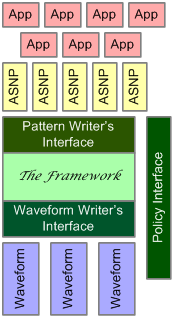
\includegraphics{figures/ASNPContext}
 \caption{Framework Design Goal}
 \label{Fig:Goal}
\end{figure}

Figure~\ref{Fig:Goal} shows the notional architecture of the
framework. Tuscarora is designed to support these broad goals:  
\begin{itemize}
 \item Scaling of MANETs: By supporting multiple patterns and even
   multiple instances of a Pattern, an application will be able to
   choose a pattern that closely matches its data distribution needs,
   thereby decreasing overhead significantly versus the traditional
   any-to-any routing approach.

 \item Portability: A standardized abstraction for Patterns makes them
   portable across platforms and waveforms.

 \item Support Heterogeneity: Standardized abstractions for waveforms
   allow any waveform that implements the abstractions to be ``plugged
   in'' to the framework.  Moreover, every Tuscarora node is a ``gateway''
   node between all supported waveforms.

 \item Flexible Management: An open policy manager that operates on
   self-describing management interfaces of modules provides a very
   flexible way of managing the network.  Further, it enables a
   human-in-the-loop management architecture to carry out network and
   mission management tasks.
\end{itemize}

To understand the design decisions better, please see the Tuscarora
Design Rationale document.

\subsection{Services}
\label{Subsec:Services}

To accomplish the foregoing goals, the framework provides the following services:
\begin{itemize}
 \item \textbf{Neighborhood service:} Discovers neighbors and evaluates the
   quality of their links; notifies Patterns (via callbacks)
   whenever there are changes in the neighborhood.

 \item \textbf{Data Flow:} Provides multi-destination send and broadcast
   services; also provides various forms of notification (acks) when messages
   are sent out and/or received at the destination.

 \item \textbf{Pattern Naming:} Provides a way of naming patterns. Multiple
   instances of the same pattern can be instantiated in the network.

 \item\textbf{ Policy Manager:} Implements a number of policies for the framework. Also provides hooks for a network manager to various other modules which might support policy definitions.
\end{itemize}


The developers of the framework have also defined a number of optional services, that might be useful or even necessary on some platforms.
These are not standardized and are not expected to be available on all platforms. Samraksh is not responsible for providing these services, however
we might provide this service as a library or specific implementations for some platforms.
\begin{itemize}
	\item \textbf{Time Stamping:} This service provides timestamps for events.  The basic idea of this service is to translate a event that happened on a (direct) neighboring node to a corresponding time on a given node. That is provide a basis for synchronization of times when time synchronization is not available already.
	Two variations are defined a explicit sender based and implicit receiver based. In the explicit sender based version, a sending node marks a Event Time, in some time unit, puts it into a packet and sends it to a neighbor. The receiver node takes a timestamp when this packet is received on the lower levels. If the delays between the sending node taking the timestamp and the receiver node taking its timestamp can be accomplished then the event times across the two nodes can be  synchronized. In implicit receiver based timestamping, the sending part is absent. The receiver is expected to know the rate or schedules  at which an packet sending event is supposed to happen on a neighbor and simply expects packets according to that schedule. The implicit timestamping service simply takes a timestamps of all incoming packets and sends them to the user of the service which can then parse these timestamps to arrive at time mapping between the two nodes.
	
	\item \textbf{Neighbor Time:} This services provides a given neighbor's time corresponding to local time. This is also called as network time synchronization service. This is expected to build on top of the timestamping service. However, specialized radios/waveforms may be able to implement this all by themselves.
	
	\item \textbf{Location:} Provides the geographical coordinates of a node. This service will need to interface with some underlying hardware such as GPS or location systems.
	
	\item \textbf{Mobility Control:} Provides the ability to move the current node to a given location or set the motions towards a given direction. Useful for nodes that can move or for mobile simulations.
	
	\item \textbf{ Global Name}: Provides a globally unique name for a node. Patterns or Apps might query this service to get a the nodes global name and use it as the identifies in its protocols and algorithms.
	
\end{itemize}


\subsection{List of Key Interfaces}

List of APIs:
\begin{itemize}
 \item  Implemented by platform Shim Layer provider
    \begin{itemize}
      \item PatternBase
      \item FrameworkShim
    \end{itemize}
 \item Implemented by Framework provider (Accessible by the Patterns)
    \begin{itemize}
      \item Framework\_I
      \item PatternNaming\_I
      \item PatternNeighborTable\_I (As a library)
    \end{itemize}
 \item Implemented by the Waveforms
    \begin{itemize}
      \item Waveform\_I
      \item WF\_LinkEstimator\_I
    \end{itemize}
\end{itemize}


List of Service APIs:
\begin{itemize}
 \item Implemented by Framework
    \begin{itemize}
      \item LinkEstimation\_I
      \item PotentialNeighborRegistry\_I
      \item NetworkDiscovery\_I (default)
      \item PolicyManager\_I
      \item NeighborTable\_I
      \item PatternNaming\_I
    \end{itemize}
 \item Implemented by external providers
    \begin{itemize}
      \item GlobalNodeName\_I
      \item LocationService\_I
      \item NeighborTime\_I
      \item NetworkDiscovery\_I (Overrides the default if available)
   \end{itemize}
\end{itemize}

\chapter {Getting Started}
\label{Chap:Install}

Tuscarora is a cross platform software system and can be used on most desktop systems. Tuscarora comes pre-integrated with ns3 simulator that can be used to test the users code. The NS3 is designed for POSIX compliant systems and hence using the installation script for simulator will require POSIX systems. However, beginning Summer 2016 Windows is expected to support a POSIX/ubuntu environment. The following section is written for Ubuntu system. Howeve, it should work on most POSIX systems.


\section{Supported Platforms}
Ubuntu 16.04 64-bit and Ubuntu 14.04 64 bit are the recommended platforms. The instructions should work on most 64-bit Ubuntu platforms with the following restrictions.  32-bit distributions are not support.

\begin{itemize}
%\item Ubuntu 15.10 is supported with the following modiufications gcc change . ..
	\item Ubuntu 16.04 is proffered developmental platform. 
	\item Ubuntu 14.10 is not a long term release and reached EOL in July 2015. This version is not supported. % ?
	\item Ubuntu 14.04: There are 6 sub-releases here, 14.04, 14.04.1, ..., 14.04.5. All of them should work with no modifications.
	\item Other 64-bit Ubuntu versions starting at 12.04 should work, although Samraksh does not officially support anything older than 14.04.
	\item Any other distribution is discouraged. If you are planning to
	  use any other platform, first check out the requirements for ns3-dce~\cite{dce}.
\end{itemize}

\section{Installation}

\subsection{Installation from Scratch} \label{subsec:InstallationFromScratch}

\begin{enumerate}
\item \textbf{Extract the source Files:} Move the Tuscarora package to
  a new directory, say `C2E'. The release file is a password-protected
  rar-archive, so you will need the \texttt{rar} package.
\begin{quote}
	\$ cd \\
	\$ mkdir C2E\\
	\$ mv Tuscarora-release-0.x-y.rar C2E\\
	\$ sudo apt-get install rar \# if not already installed\\
	\$ rar x Tuscarora-release-0.x-y.rar\\
\end{quote}

\item \textbf{Launch installation:} The previous step will create a Tuscarora directory, this is the root of the framework. Launch the `install.sh' script under 
Tuscarora root directory. 
Since the script adds some environment variables, it has to be called within the same shell. Please note the ``.'' before the command. 
If not, a new shell should be started after the installation completes in order to set the environment variables. 
\begin{quote}
	\$ cd TuscaroraFW\\
	\$ . ./install.sh\\
\end{quote}
\item \textbf{Installation:}  The installation script will ask for
  your `sudo' password for installing some dependencies. Enter your
  password. The script will download and install the required ubuntu dependencies
  first. Next, it will proceed to download and install bake, ns3, and
  dce from the nsnam repositories. Ns3 and dce will be installed under
  a directory called `dce' under your home directory; let's call this
  the \$DCE\_DIR directory. Next the script will make some symbolic
  links between the Tuscarora source directory and the
  \$DCE\_DIR. Finally, if all previous steps work fine, it will run
  some existing modules, and will return the status of execution.
% XXX status of execution, or status of installation?

\end{enumerate}


\subsection{Upgrading from Previous Release}
To upgrade from an existing Tuscarora installation following the procedure below. 
\begin{enumerate}
	\item \textbf{Remove and Replace Tuscarora Directory}: Follow the path, where Tuscarora was installed, say C2E, and replace the Tuscarora directory with the contents of the new package. 
	\begin{quote}
		\$ cd C2E\\
		\$ rm -r Tuscarora\\
		\$ sudo apt-get install rar \# [if not already installed]\\
		\$ rar x Tuscarora-release-x.y-z.rar\\
		\$ cd Tuscarora/TuscaroraFW \\
	\end{quote}
	
	\item \textbf{Reinstallation}: Before we can install the new version, the ns3/dce patches from previous version should be removed first. To do this:

	\begin{quote}
		\$ cd Tuscarora/TuscaroraFW \\
		\$ ./install.sh -u  \# [this will remove the patches]\\
	    \$ ./install.sh \\
	\end{quote}
\end{enumerate}


If at any stage you encounter error, please contact support.


\subsection{Validating the installation}
Finally, once the installation finishes, you can validate the installation by running the command ``./validate.sh'' from the TuscaroraFW directory followed by ``-p platform'' option. This would run a number of predefined validation tests for the given platform and would print the result of the tests as FAILED or PASSED on the screen. If any of the tests fail, please contact support. Running the validate script with the `-h' option prints the list of validation tests available.


\section{Executing Tuscarora Framework Modules}

The `runOrDebug.sh' in the root directory is the primary script to execute the modules and tests under framework. The script cleans, builds, runs and collects the output for the 'test-name' specified. 
Run the script without parameters for information on supported options. Run the script with the test-name and `-h' option to get test-specific help.

% XXXX GIVE MORE INFO about options, e.g., put general ns3 options
% before the '--' and sim-specific options after.

\subsection{Example Executions}


0. Getting help for the usage of runOrDebug.sh, to find the list of available tests.

\begin{quote}
	\$ ./runOrDebug.sh  \\
\end{quote}

1. Getting help for Gossip test, to find the list of all test parameters with their default values.

\begin{quote}
	\$ ./runOrDebug.sh -h Gossip  \\
\end{quote}

2. Running the Gossip pattern test for 60 secs on a 100 node network.

\begin{quote}
	\$ ./runOrDebug.sh Gossip -\mbox{}- RunTime 60 Size 100\\
\end{quote}


3. Running the Gossip pattern test inside the gdb to debug for 100 nodes (and a default duration of 6 secs).

\begin{quote}
	\$ ./runOrDebug.sh -d Gossip -- Size 100\\
\end{quote}


4. Running the Framework Interface test `FI' with Periodic Link Estimation with a dead neighbor period of 2 seconds and a Link Estimation Period of 1Hz using Global Network Discovery.

\begin{quote}
\$ ./runOrDebug.sh FI -\mbox{}- LinkEstimationType periodic LinkEstimationPeriod 1000000 DeadNeighborPeriod 2 DiscoveryType global\\
\end{quote}
	
5. Running the Framework Interface test `FI' with Schedule Aware
Periodic Link Estimation, a Link Estimation Period of 10Hz, and
2-hop Long Link Network Discovery.

\begin{quote}
\$ ./runOrDebug.sh FI -\mbox{}- LinkEstimationType
scheduleAwarePeriodic LinkEstimationPeriod 100000 DiscoveryType longlink2hop
\end{quote}
	

6. Running the Gossip pattern test with 10 nodes with a waveform configuration file.

\begin{quote}
	\$ ./runOrDebug.sh Gossip -- Size 100 WFConfig ~\$\{TUS\}/dceln/wf-config.cnf  \\
\end{quote}

7. Running the Gossip pattern test with a tracefile based mobility model. The tracefile needs to be in the ns-2 mobility trace file format.

\begin{quote}
	\$ ./runOrDebug.sh Gossip -- Size 10 RunTime 10 Mobility TracefileMobilityModel Tracefile ~\$\{TUS\}/TraceFiles/Simple-Size10-10secs.tr  \\
\end{quote}


For more information on running Tuscarora on various platforms, testing methodology and configuration options see Chapter~\ref{Chap:Exec}.

\section{Execution Output Files}

The runOrDebug script creates outputs in the directory ``dceln''. This directory is a symlink to the main dce execution directory, which is located at ``\$HOME/dce/sources/ns-3-dce''. 

Under this directory you will find a number of outputs generated:

%The ability to create outputs as a memory map binary file will be enabled in the next release. 

\begin{itemize}
	\item time.output: This file summarizes the high level information about the test such seen from the operating system such as the command being run, its terminating condition, the time it takes to complete, the amount of system resources used, etc. 
	\item simulation\_description: This file details various features of the simulation either set by the command line arguments or used as the default values. 
	\item exitprocs: This file stores information about the execution process. 
	\item CourseChangeData.txt: This file stores information about the mobility. More specifically, for each change in the velocity of a node, a line of record indicating the time instances, node's ID, node's new velocity and node's location at that time instant is stored.
	\item elf-cache: The compiled program files are stored under this directory. 
	\item file-x: Directories such as files-0, files-1, etc., store the file system of each simulated node. 
	Each of these directories have a simulation\_desciription file identical to the one located at \FilePath{\$HOME/dce/sources/ns-3-dce}. 
	In addition to that, the generated data at each node is stored in these directories.  
	"Configuration.bin" stores the configuration parameters in binary format.
	"linkestimation.bin" stores the link estimation state in binary format. 
	The output for each node can be found under file-*/stdout. 
	This file stores the outputs of the ``Debug\_Printf'' macro or the ``printf'' to ``stdout'' of each node during the simulation. 	
\end{itemize}

\section{Directory Structure}

\begin{itemize}
\item Config: Sample waveform configuration files for simulation
\item Doc: Documentation
\item Install: Scripts to automate installation of Tuscarora
\item Include: Header files / API specifications
\item Lib : Platform neutral library modules
\item ns-3-dce: Simulation scripts to run under dce
\item Patchs: Patches to DCE module to enable additional features %{\bf (Will be depreciated in future releases)}
\item Patchs.ns3: Patches to the ns-3 modules.
\item Platform: Platform-specific library modules
\item Scripts: Various utility scripts
\item Src: Framework and Pattern source files
\item Tests : Tests for modules, layers and patterns
\end{itemize}

\section{Compilation, Linking and Execution Details}\label{CompilationDetails}

Tuscarora's framework links with DCE source tree through the \$TUS/ns-3-dce/myscripts/TuscTest folder.  A link for this folder is created in the ``\$DCE\_DIR/sources/ns-3-dce/myscripts''.
This folder includes c++ programs defining ns3 simulation environment to be used in the simulation. 
The defaults setup of the runOrDebug.sh script uses the ``tuscarora-test.cc'' program that sets ns3 and DCE setup for the simulation depending on the run time arguments. It is compiled through waf system of the DCE and its binary is placed under ``\$DCE\_DIR/build/bin''.

While executing a program using the DCE framework, the test program written using Tuscarora is compiled as a dynamically linked shared library and loaded into the DCE environment. Notionally, DCE provides the ``OS'' and  the tests written using Tuscarora are like "application" executed on that OS. DCE provides these ``OS services'' by utilizing either ns-3 modules or by using the native linux services.

One difference between DCE and an actual OS is that DCE "runs" multiple copies of the application, one per node, while an actual OS would run only one copy. 

The actual test/simulation that is run on top of DCE can be controlled by the Test parameter provided to the runOrDebug.sh script. ``TuscaroraFW/Tests'' folder includes a number of programs intended to be used as test applications. Each such program has its own main() function, which is where a given node's execution begins.


%Essentially, they implement the main to be run at a node.
%These tests are compiled separately by the runOrDebug.sh script and the binaries are copied under  ``\$DCE\_DIR/sources/ns-3-dce/build/bin\_dce''. The framework and the patterns used by this program is provided as a DLLs. 

Finally, the source code for the framework and the source code for the sample patterns provided reside in ``TuscaroraFW/Src''. As explained above, depending on the test program being run, these individual tuscarora modules are compiled and linked into DLL binary by the runOrDebug.sh  script and an associated Makefile and are placed under ``\$DCE\_DIR/sources/ns-3-dce/build/bin\_dce''. These binary DLLs are loaded into a ns3-dce binary executable which is usually called ``tuscrora-test".

A typical simulation consists of following run-time threads:
\begin{itemize}
\item Initially, a single thread starts  and runs the code in tuscarora-test. This thread act as the overall manager of the simulation, and does coordination between nodes, and also runs ns3 module code (simulating the waveform(s), the channel(s), nodes, events, etc.). 
\item With the start of the ns3 simulation,  for each node a separate thread is created, which runs test program specified as the run time argument.
\item The test program running on each node creates instance(s) of the pattern(s), an instance of the framework and instance(s) of the waveforms layer are created.
\end{itemize}
%ADD a figure showing the interactions

\chapter{Inter Layer Messaging and Build Options}
\label{Chap:ILS}


Tuscarora provides a flexible deployment procedure in which modules depicted in \cref{Fig:Goal} can run in their own processes or several of these modules can be bundled to share a single process. 
In order to enable deployments on various platforms and 
to provide a common architecture for single process or multi-process setups, 
Tuscarora defines a communication module that translates calls between various layers. We colloquialy refer to this as the ``communication shim layer'' or just as ``shim''; 
A shim layer is required  between the applications and the patterns, between the patterns and the framework, and between the framework and waveforms as shown in \cref{fig:CommonShimLayerInterface}.

Tuscarora APIs are designed with function syntax(aka method calls) and named with message passing semantics.
The job of the shim layer is to translate a function call from within one layer to a function call on another layer, using asynchronous message passing between layers.
For example, a pattern makes a call to a shim layer object and the shim layer object calls the framework, which might be part of the same process space or might be running as a different process. For multi-process environments,
this shim layer should convert the function calls to messages or some other inter-process mechanism (such as pipes) and send them to the corresponding modules on the other layer.
Similarly, the shim layer parses and converts received messages back into function calls and invokes the corresponding functions on the receiving layer.

\begin{figure}[ht]
	\centering
	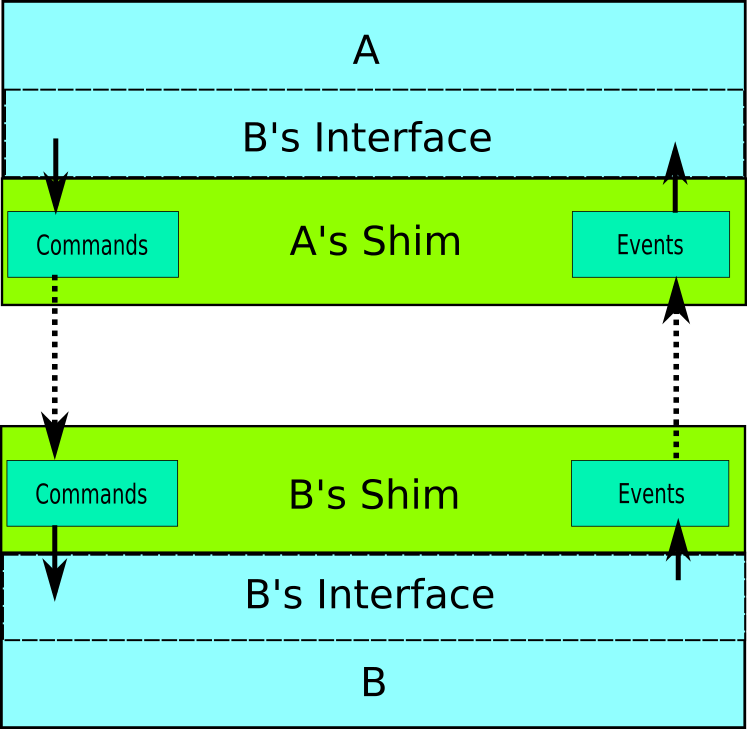
\includegraphics[width=0.3\linewidth]{figures/CommonShimLayerInterface}
	\caption{Generic example of Shims between Layer A and Layer B, where A is user of B}
	\label{fig:CommonShimLayerInterface}
\end{figure}


In a single-process environment, a shim layer can be implemented using one of the many different options available, such as synchronous blocking function call, asynchronous non-blocking function calls, messaging passing or signaling.
In general, the implementation of these shim layers can be platform-specific and when porting Tuscarora to a new platform at least some of the shim layer modules may need to be reimplemented.
Tuscarora interfaces are designed with `Commands' that are received by a module and `Events' that are invoked or sent from a module, i.e., Tuscarora interfaces are bidirectional. For example, consider two layers , A and B, as shown in \cref{fig:CommonShimLayerInterface}. 
If layer A wants to invoke a command on layer B, then a communication shim is need both on A's side to send out the Commands and to receive  B's Events. On B's side we need a shim to receive the commands and to send out the Events. 
However, sometimes (mostly in single process case), the shim on either A or B can be skipped, if they have a common shared memory location. 
The Shim on A's side should implement B's interfaces, both Commands and Events. 
That is A's shim translates from B's interface to some common agreed upon communication standard between A and B, and B's shim translates back this communication standard back to B's interface specification and invokes B.  Therefore A's shim looks like B to A.


Tuscarora package provides shim layers designed for the DCE environment as well as linux multi-process environments. 

\section{App-Pattern Shim Layer Modules}

Applications can be written towards the interface definitions of one or more patterns. 
Depending on the platform, the object implementing the interface could be the pattern itself or a pair of shim layers that pass the call to the intended pattern. \Cref{fig:AppPatternInterface} depicts setups for multi-process and single process environments. 

\begin{figure}[ht]
\centering
	  \begin{minipage}[b]{0.4\textwidth}
	    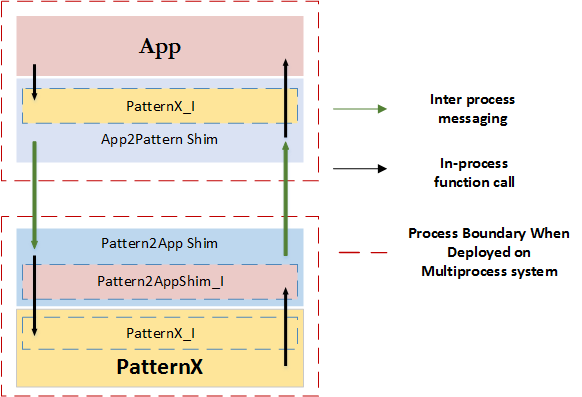
\includegraphics[width=\textwidth]{figures/App_Pattern_ShimArchitectureMP}
	    %\caption{multi process platform}
	    %\label{fig:AppPatternInterfaceMP}
	  \end{minipage}
	  \hspace{5mm}
	  \begin{minipage}[b]{0.4\textwidth}
	    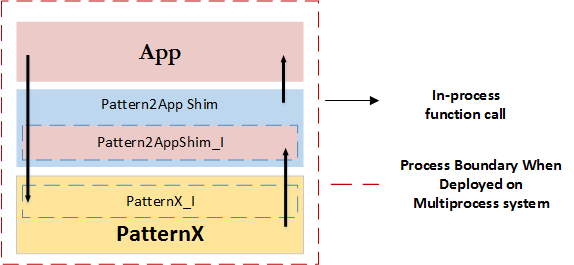
\includegraphics[width=\textwidth]{figures/App_Pattern_ShimArchitectureSP}
	    %\caption{single process platform}
		%\label{fig:AppPatternInterfaceSP}
	  \end{minipage}
\caption{App-Pattern interface for multi process and single process environments}
\label{fig:AppPatternInterface}
\end{figure}


\subsection{Multi process Shim Setup}

In multi process environments, \CPPClassName{App2PatternShim} and \CPPClassName{Pattern2AppShim} \CPPClassName{App2FWPShim} pair carry calls from each side of the process to the other side. Internally, these calls are converted to serialized messages on the sending side and carried over using a socket communication interface. Once received, the message is deserialized and the destination layer is called with the variables inside message. 

Tuscarora provides \CPPClassName{SocketCommunicatorClientBase} and the \CPPClassName{SocketCommunicatorServerBase} classes to automate server-client connection process, and \CPPClassName{GenericSerializer} and \CPPClassName{GenericDeSerializer} templated classes that help serialization and deserialization process for the shim classes. 


\CPPClassName{SocketCommunicator} library simply provides functions to send serialized buffers to the other side and on receiving event it directs read contents to a virtual \CPPFuncName{Deserialize} function implemented by the corresponding shims. 

A generic serializer object is simply constructed by listing the list of variable types and the corresponding variables and it creates a serialized buffer that contains copies of the variable values. Similarly, a generic de-serializer deserializes a variable sized buffer by copying its content to individually created variables in the order specified in its constructor. They also accepts pointers in which case the value of the preceding variable is assumed to be the size of the object pointed by the pointer. 


We'll elaborate this process with an example call to SendData from the \TuscConcept{FanOutFWP} application to \TuscConcept{FWP} pattern. 

\CPPClassName{App2FWPShim}'s \CPPFuncName{SendData} uses a GenericSerializer object to create a serialized buffer consisting of a calltype, and the function inputs, namely \CPPVarName{AppId\_t}, the variable sized message and a nonce that is used to identify the message between the app and the pattern. Then \CPPClassName{App2FWPShim} calls the \CPPFuncName{SendMsg2Server} function implemented by the base class, \CPPClassName{SocketCommunicatorClientBase}, to send the serialize message to the corresponding server.

Upon receiving the signal ,the message contents are read from the socket by \CPPClassName{FWP2AppShim}'s base class \CPPClassName{SocketCommunicatorClientBase} and \CPPFuncName{Deserialize} function of \CPPClassName{FWP2AppShim} is invoked. \CPPFuncName{Deserialize} function, first reads the calltype from the received buffer. Depending on the calltype, the rest of the buffer is deserialized into individual variables. In the case of the calltype being \CPPVarName{APP2FWP\_Call\_Send}, the rest of the buffer is deserialized into an \CPPVarName{AppId\_t}, a variable sized message and a nonce using a \CPPClassName{GenericDeSerializer}. Using these variables, the  \TuscConcept{FWP} pattern's \CPPFuncName{SendData} function is invoked. Hence, the call from \TuscConcept{FanOutFWP} to \TuscConcept{FWP} is completed. 


\subsection{Single process Shim Setup}

In single process setups, such as the ones DCE platform uses, \TuscConcept{App2PatternShim} disappears and the function calls directly invokes implementations in the \TuscConcept{PatternX} as depicted in \cref{fig:PatternFrameworkInterface}. \TuscConcept{Pattern2AppShim} only acts as a dispatcher or a multiplexer by invoking applications registered to the pattern. 

We'll elaborate this process with an example call to \CPPFuncName{ReceiveUpdatedGossipVariable} from the \TuscConcept{Gossip} pattern to \TuscConcept{BasicGossipApp}. 

During the initialization, \TuscConcept{BasicGossipApp} registers its delegate used for receiving updates by invoking \CPPFuncName{RegisterGossipVariableUpdateDelegate} method of the \TuscConcept{Gossip} pattern. \TuscConcept{Gossip} redirects delegates to the \CPPClassName{Gossip2AppShim}, where they are stored for further use. 

Whenever there is an update to the internal variable being, \TuscConcept{Gossip} invokes  \CPPFuncName{ReceiveUpdatedGossipVariable} in \CPPClassName{Gossip2AppShim}, which in turn invokes the list of delegates stored. 


\section{Pattern-Framework Shim Layer Modules} \label{sec:PatFrameworkInterface}

%\begin{figure}[ht]
%	\centering
%	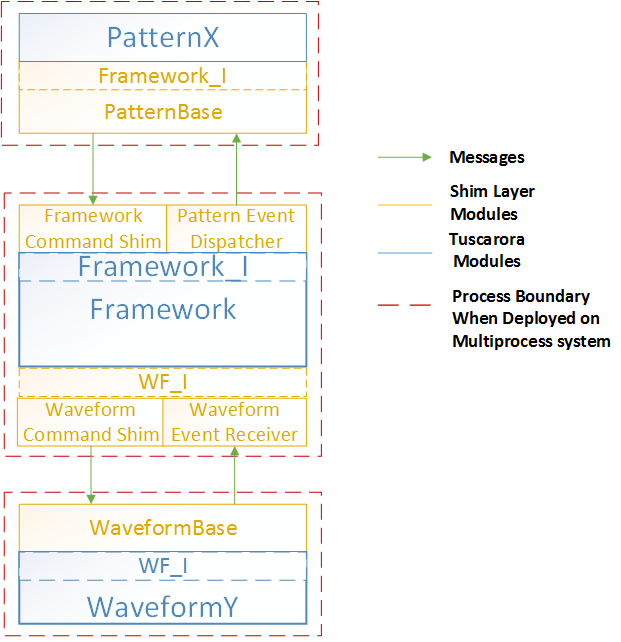
\includegraphics[width=0.7\linewidth]{figures/ShimArchitecture}
%	\caption{Pattern-Framework-Waveform interface}
%	\label{fig:ShimLayerInterface}
%\end{figure}

\begin{figure}[ht]
\centering
	  \begin{minipage}[b]{0.6\textwidth}
	    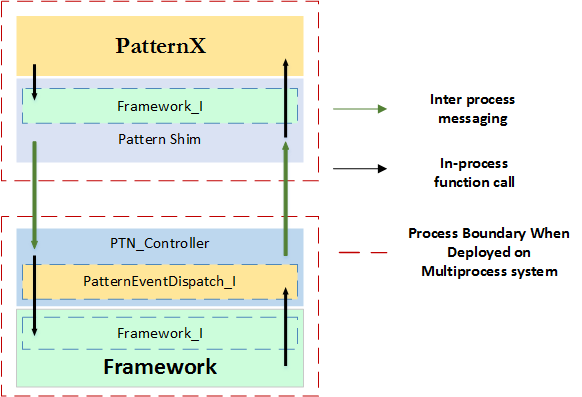
\includegraphics[width=\textwidth]{figures/Pattern_Framework_ShimArchitectureMP}
	    %\caption{multi process platform}
	    %\label{fig:PatternFrameworkInterface-MP}
	  \end{minipage}
%	  \hspace{3mm}
	  \begin{minipage}[b]{0.6\textwidth}
	    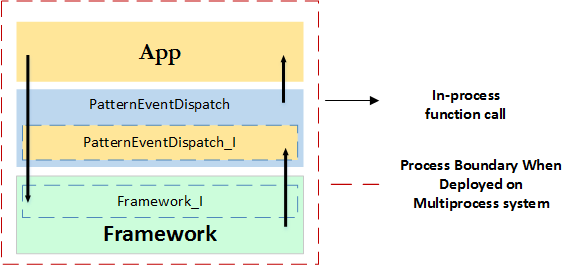
\includegraphics[width=\textwidth]{figures/Pattern_Framework_ShimArchitectureSP}
	    %\caption{single process platform}
		%\label{fig:PatternFrameworkInterface-SP}
	  \end{minipage}
\caption{Pattern-Framework interface for multi process and single process environments}
\label{fig:PatternFrameworkInterface}
\end{figure}

In order to facilitate the Pattern development, Tuscarora package comes with a common base class library, namely \CPPClassName{PatternBase}, that automates connections in the Pattern-Framework interface. For patterns deriving from it,  \CPPClassName{PatternBase} choses the shim classes required by the platform, initiates the communication medium with the Framework and provides patterns an abstracted pointer to the Framework through a member variable called \CPPVarName{FRAMEWORK}. Thus, for convenience Patterns are expected to inherit from \CPPClassName{PatternBase}, although it is not strictly necessary, 

The implementation of \CPPClassName{PatternShim} is platform-specific since implementing the Framework\_I interface to communicate with the actual framework will depend on the types of communication mechanisms available on a given platform. PatternBase also receive the \CPPClassName{Framework\_I} Events and convert them back into delegate calls for the Patterns. The corresponding Shim layer on the framework side is implemented by two classes-- one for Commands by the \CPPClassName{FrameworkShim} and one for Events by the \CPPClassName{PatternEventDispatch}. \Cref{fig:PatternFrameworkInterface} shows the flow of messages and bindings for this scenario..

In the DCE, the shim layers are implemented using synchronous function calls, since they are part of the same process space as shown in \cref{fig:PatternFrameworkInterface}. PatternBase gets a pointer directly to the FrameworkShim class (which is the shim class on the framework side) and invokes commands on it. Similarly the PatternEventDispatch module gets access to the Delegate objects in PatternBase and directly invoke them to implement the Events. 
 
\section{Framework-Waveform Shim Layer Modules} \label{sec:WaveformFrameworkInterface}
 
For the shim layer between the Framework and Waveform, the \CPPClassName{WF\_Controller} implements the commands in the WF\_I interface and ``Waveform Event Receiver'' module implements Events in WF\_I interface. 

On the waveform side the commands are directly provided by the modules that implement the WF\_I (i.e no shim in the forward direction in necessary) and the Events part of the WaveformBase shim are implemented \CPPClassName{AsyncEvent\_Special} module.

Once again, since in DCE we are in a single process address space, the shim modules directly get access to the objects on the other side and invoke them. The multi process and single process case interfaces are depicted in \cref{fig:FrameworkWFInterface}.

\begin{figure}[ht]
\centering
	  \begin{minipage}[b]{0.4\textwidth}
	    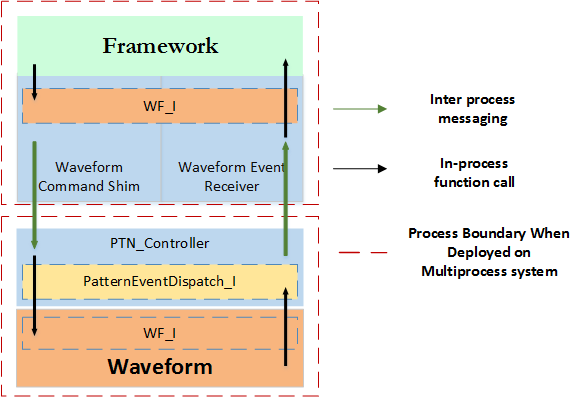
\includegraphics[width=\textwidth]{figures/Framework_Waveform_ShimArchitectureMP}
%	    \caption{multi process platform}
	%    \label{fig:FrameworkWFInterface-MP}
	  \end{minipage}
	  \hspace{5mm}
	  \begin{minipage}[b]{0.4\textwidth}
	    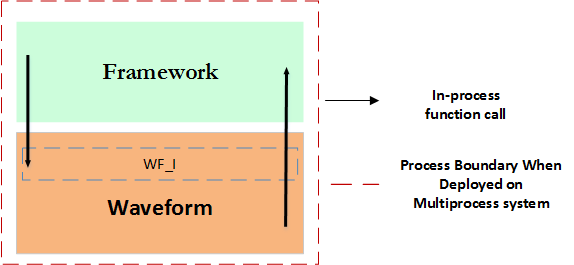
\includegraphics[width=\textwidth]{figures/Framework_Waveform_ShimArchitectureSP}
	    %\caption{single process platform}
		%\label{fig:FrameworkWFInterface-SP}
	  \end{minipage}
\caption{Framework-Waveform interface for multi process and single process environments}
\label{fig:FrameworkWFInterface}
\end{figure}


\iffalse 
The interface controlling messaging from the \TuscConcept{Framework} to the \TuscConcept{waveforms} is declared in \CPPClassName{Waveform\_I}. The framework keeps a pointer to this interface and simply invokes the functions declared in \CPPClassName{Waveform\_I}.

The messaging from the \TuscConcept{waveforms} to the \TuscConcept{Framework} is handled by the declarations provided by the templated class \CPPClassName{WF\_Event}. 
\CPPClassName{Waveform\_I} declares separate event types for various events such as 
\begin{itemize}
\item received message event (\CPPClassName{WF\_RcvMessageEvent\_t}), 
\item data notification event (\CPPClassName{WF\_DataNotifierEvent\_t}), 
\item link estimation event (\CPPClassName{WF\_LinkEstimateEvent\_t}),   %(WF_LinkEstimateEvent_t)
\item control response events (\CPPClassName{WF\_ControlResponseEvent\_t}), and
\item schedule update event (\CPPClassName{WF\_ScheduleUpdateEvent\_t}).
\end{itemize}
The waveform creates an event object of the corresponding type and a parameter object that is initialized with the information that is being transferred to the \TuscConcept{Framework}. 
Once the parameter is initialized, the waveform can simply invoke the event with the parameter. 
The event class the information using the shim layer to the Framework,
where it will be routed to the particular module that will process the received waveform data message. 
\fi


%/**
%  # Received Message Event #
% ## Invoke Method Definition ##
% * bool WF_RcvMessageEvent_t::Invoke (WF_RecvMsgParam param);
% * 
% * The Received Message Event class has a single public method called Invoke, which can be use do send the event to the framework, with WF\_RecvMsgParam as
% * the parameter.
% ## Expected Behavior: ##
% * When the waveform receives a valid data message through its radio interface, the waveform should event the Framework using the ``Receive Message Event''.
% * Upon receipt of a message, waveform will evaluate metadata (RSSI, SINR, Receive Timestamp) associated with the message and the metadata will be added to
% * the packet structure and passed in the parameter to the event.
% * An operating mode wherein the waveform forwards up to the Framework each and every packets that it receives and decodes correctly irrespective of whether
% * the packet was destined for the node is commonly referred to as ``promiscuous mode''. The API does not take a position on whether or not waveforms should
% * support promiscuous mode. (Hence, no API is currently defined to configure such a mode). If a future programmatic decision is made to support promiscuous
% * mode of waveforms, a policy manager (through the Framework) will explicitly configure the waveform to operate in such a mode. Unless explicitly configured
% * a waveform should not send packets not intended for the node to the Framework.
% * Note to Pattern designers: If a waveform does send packets to the Framework that are not meant for a particular node, the Framework has no way of identifying
% * such packets. The Framework cannot guarantee to a Pattern that it will not receive such “unintentional” packets. If a Pattern does receive such packets they would have originated from the same Pattern instance on a neighboring node, but are not intended to be received on the current node (i.e., right pattern, wrong node). We recommend that Pattern designers consider the possibility of receiving some unintentional packets and make their patterns robust enough to handle them.
% ## Event creation and invocation: ##
% * The details of the WF_RecvMsgParam parameter, and the code for creation and invocation of the Received Message are shown below. The waveform provider
% * creates the event object and the parameter object. Further, it initializes the parameter object with the received data message, the rcvMsgId is assigned
% * a MessageId generated by the waveform for the messages received by it. Once the parameter is initialized, the waveform can simply invoke the event with the parameter. The event class will convert this into a message of the appropriate format and send it using the shim layer to the Framework,
% * where it will be routed to the particular module that will process the received waveform data message.
% 
% #  Data Notification Event #
% ## Invoke Method Definition ##
% * bool WF_DataNotifierEvent_t::Invoke (WF_DataNotifierParam param);
% * The Data Notification class has a single public method called Invoke, which can be use do send the event to the framework, with WF_DataNotifierParam as
% * the parameter.
% ## Expected Behavior:
% * When a ‘SendData’ or ‘BroadcastData’ command is received by the Waveform, the Framework expects a Data Notification Event in response. The ackType in the parameter of the Data Notification Event indicates the type of notification. For each SendData command received with a particular MessageId, the waveform should send back at least two events, one of the ACK_WF_RECV type, indicating that the waveform received the message successfully and one of the ACK_WF_SENT type, indicating the waveform sent the message out through its radio. A third type named ACK_DST_RECV can also be sent if the waveform supports acks from the destination. For the BroadcastData command, the first two types are required and the third is not required. The ‘dest’ field in the param is an array that determines for which destinations that notification is being sent. For example, if the Waveform chooses to send multiple physical messages corresponding to the same “MessageId” once for each destination, then a notification event can be sent once per destination or it can all be grouped together and sent as a single notification.
% ## Event Parameters:
% * The parameter creation and invocation is quite similar to that of the other events. The waveform needs to create an object of WF_DataNotifierEvent_t,
% * create an object of the WF_DataNotifierParam and invoke the event with the param. The parameter for this event is show below.
% 
% # Link Estimation Event
% ## Invoke Method Definition
% * bool WF_LinkEstimateEvent_t::Invoke (WF_LinkEstimateParam param);
% * The Link Estimation Event class has a single public method called Invoke, which can be use do send the event to the framework, with WF_LinkEstimateParam as the parameter.
% ## Expected Behavior:
% * Link estimation of known neighbors is an optional function that the waveforms can choose to provide. If supported, the waveform should set the ‘estType’ field in its Attribute to WF_EST_FULL whenever it responds to the AttributeRequest.
% * Waveform that provide link estimation should provide link estimation events, and follow a standard format. The Framework defines a link metric structure that the waveform should compute for each neighbor. The WF\_LinkMetrics structure is show below, it consist of four metrics that are defined as follows:
% * 1. Quality: Abstract quality metric expressed as a real number between [0,1].
% * 2. Data rate: Link data rate expressed as log_2(bps).
% * 3. Average Latency: Average latency in sending a packet to the destination expressed as log_2(seconds).
% * 4. Energy: Average energy to transmit a packet expressed as log_2(pica-joules).
% * 
% The waveform is expected to generate a event for each neighbor whenever one of the three events happens:
% * 1. New Neighbor: Whenever the waveform detects a new neighbor and has an initial estimate of its link metrics. It uses the value NBR_NEW for the ‘changeType’ field of the event parameter.
% * 2. Dead Neighbor: Whenever a previous neighbor no longer exist in the neighbor. Use the value NBR_DEAD for the ‘changeType’ field of the event parameter
% * 3. Change in Metrics: Whenever the metrics has changed enough to notify the Framework. It uses the value NBR_UPDATE for the ‘changeType’ field of the event parameter.
% ## Event Parameters:
% * The  WF_LinkEstimateParam structure (shown above) is used as the parameter for the Link Estimation Event. The structure contains the waveform address, the link type, its link metrics and the type of change in neighborhood being conveyed by the message.
% # Control Response Event
% ## Invoke Method Definition
% * bool WF_ControlResponseEvent_t::Invoke (WF_ControlResponseParam param);
% * The Control Response Event class has a single public method called Invoke, which can be use do send the event to the framework, with WF_ControlResponseParam as the parameter.
% ## Expected Behavior:
% * Whenever a waveform receives any request command, i.e., a command whose name has the suffix Request, it should use the Control Response Event to send a response. The response should use the same “RequestId” as in the request command. The Framework tracks the RequestId that it uses for each waveform and generates a new RequestId for every request command. If the Framework fails to receive a response for a request, the Framework may resend the request using the same RequestId.
% ## Event Parameters:
% * The WF_ControlResponseParam parameter associated with the Control Response is shown below. The key field is ‘type’, which is an enum of type WF_ControlResponseE. This enumerator defines a response for each of the Request commands. The waveform should set this type appropriately based on the command it is responding too. The parameter also contains a generic ‘data’ field, whose interpretation by the Framework depends upon on the type of the response. Based on the type of Request command that is being responded to, an appropriate structure is copied into the ‘data’ field, and the number of bytes sent through the data field should be set appropriately in the dataSize  field.
% 
% # Schedule Update Event
% ## Invoke Method Definition
% * bool WF_ScheduleUpdateEvent_t::Invoke (WF_ScheduleUpdateParam param);
% * The Schedule Update Event class has a single public method called Invoke, which can be use do send the event to the framework, with WF_ScheduleUpdateParam as the parameter.
% ## Expected Behavior:
% * Schedule updates are an optional feature by which waveforms that maintain schedules for functions such as sending, receiving or link estimation can share information about the schedules with the Framework. If the feature is supported, the waveform should set as true the ‘schedulerInfoSupport’ field in its Attribute whenever it responds to the AttributeRequest.
% * This event is expected to be implemented by waveforms that have timing characteristics or TDMA schedules. The eventing should be implemented if the knowledge of a waveform's slot schedules will help the Framework in improving the overall data efficiency.
% * Note: If the waveform is responding to the ‘ScheduleRequest’ command, then it should use the Control Response Event; and, if it is sending ongoing schedule updates, it should use the Schedule Updates Event.
% ## Event Parameter
% * The WF_ScheduleUpdateParam structure that is used as the parameter of the Schedule Update Event is shown below. The parameter contains information about one of three types of schedules,  send, receive or link estimation, which is indicated by setting the ‘type’ field appropriately. The ‘data’ field is a pointer of type ScheduleBaseI which points to the object that contains the actual schedule information for the neighbor indicated by ‘nodeid’. 
% * The dataSize field contains the size of the actual schedule object that is pointed to by the data field.
% */
% 



\section{NS3-DCE}

For portability reasons, this release uses the Direct Code Execution (DCE)~\cite{dce} environment for running simulations. 
DCE is a module that enables ns-3 simulator to run existing source code that is targeted towards POSIX environments. 
%In short, DCE lets users develop code that can be directly deployed on POSIX systems or run them in simulation. 
The executable for each node runs on a separate process and these processes are coordinated through another process running ns3 simulator.  
%\section{Message Passing Interfaces}
For more information see the DCE documentation~\cite{dce}.



%\section{Typical Deployment Scenarios}
%\input{DeploymentScenarios}
%\section{Implementing a Multi-process Shim}

\chapter{Application Development}
\label{Chap:Architecture}

Rather than building up applications around the idea of peer to peer communications, Tuscarora adopts the concept of using information distribution strategies provided by ASNPs. 
As shown in \Cref{Fig:Goal}, applications are positioned on top of the ASNP's in Tuscarora system architecture. 
Applications should use one or more of these underlying ASNPs for it information distribution and gathering needs. 
Hence, it is critical for an application developer to develop her applications around information flows rather than P2P communication. 
This isolates the information flow needs from the rest of the application. 
If this need cannot be fulfilled with the existing ASNPs, the information flow can be implemented as a new ASNP. 



In this chapter, we present the available ASNPs as well as envisioned ASNPs for application developers and provide examples of how applications can interact with ASNPs. 
The Application Writters Interface (AWI) is the namespace that exposes the
services of the patterns to the applications. 
The core API for the patterns are defined in their respective interface definitions
PatternX\_I. 
For full API documentation please refer to the companion document ``Tuscaroro API documentation''.

\section{Patterns Available in Tuscarora Package}
 
Out of the box, Tuscarora package comes with 2 ASNPs,
\begin{itemize}
\item Gossip: Gossip pattern stores some common information and distributes that information by infrequent random updates in the network. Internally stored Gossip information is updated with the received information only if the received data is larger than the existing one based on a customizable comparator. For slowly changing data, the last state of the data is eventually distributed to all connected nodes.

\item FWP: The Flooding with Pruning (FwP) pattern distributes a dataset generated (or aggregated) at a
node to all nodes in some “region”. The addition of pruning ensures efficient distribution of the data by limiting retransmission on the nodes that does not improve the nodes that do not have the information.

\end{itemize}


%\begin{itemize}
%\item Gossip: A shared data structure is gossiped in the network. For slowly changing data, the last state of the data is eventually distributed to all connected nodes. 
%\item FWP: This pattern implements a simple network wide flooding data distribution strategy with basic suppression of broadcasting on unused nodes. 
%\end{itemize}


\subsection{Gossip}

Gossip is a templated class that allows distribution of various data types in the network. An application writer has to specify a data type of his choice, \CPPTemplateName{GOSSIPVARIABLE}, and can optionally specify a corresponding comparator, \CPPTemplateName{GOSSIPCOMPARATOR}, which implements a \CPPFuncName{LessThan} and a \CPPFuncName{EqualTo} functions. 
In the case of receiving updates from other nodes or from local applications, this comparator is used. Comparator specification can be skipped in which specified gossip variable's \CPPFuncName{operator==} and \CPPFuncName{operator$<$} are used. 

\CPPClassName{Gossip\_I} interface defines the following:
\begin{itemize}
		
	\item \CPPSingleLine{typedef Delegate<void, GOSSIPVARIABLE&> GossipVariableUpdateDelegate_t} : is a delegate storing the callback function pointer that is invoked when there is a change in the GOSSIPVARIABLE. This callback function should have void return type and should accept a single input of type \CPPTemplateName{GOSSIPVARIABLE}.
	

	
	\item  \CPPSingleLine{void RegisterGossipVariableUpdateDelegate(GossipVariableUpdateDelegate_t* _gvu_del)} : is the method to receive the delegates sent to the Gossip pattern. Applications that desire to receive updates on the gossip variable use this method to register to the incoming information flow using this method. The Gossip pattern stores delegates it receives with this method and invokes them whenever there is an update on \CPPVarName{gossip\_variable}.
	
	
	\item  \CPPSingleLine{void UpdateGossipVariable(GOSSIPVARIABLE& newgossipVariable))} : is a method used by the applications to update the underlying \CPPTemplateName{GOSSIPVARIABLE} of the pattern.
	This method lets a application to request changing the variable being gossiped with a newVariable. 
	The newgossipVariable is compared with the existing one. 
	
	\begin{itemize}
		\item 	if the existing variable is larger(based on the comparator), no further action is taken. 
		\item   if the new variable is larger(based on the comparator), the gossip variable is updated, and all registered delegates are invoked with the new \CPPTemplateName{GOSSIPVARIABLE}.
	\end{itemize}
	
\end{itemize}


%\lstinputlisting[label=List:GossipI.h]{../../Include/Interfaces/AWI/Gossip_I.h}

\subsection{Flooding with Pruning}

The interface for FWP pattern is defined by \CPPClassName{Fwp\_I}, which declares the following:

\begin{itemize}

	\item \CPPSingleLine{typedef Delegate<void, void* , uint16_t> AppRecvMessageDelegate_t} : is a delegate storing the callback function pointer that is invoked when data is received. This callback function should have  \CPPSingleLine{void} return type and 2 inputs, namely a \CPPSingleLine{void*} pointer and a  \CPPSingleLine{uint16_t} type specifying the size of the data.
	
	\item \CPPSingleLine{void RegisterAppReceiveDelegate(AppId_t _app_id, AppRecvMessageDelegate_t* _gvu_del)} : 
	is the method to get the delegates for the \CPPClassName{FWP} pattern. The delegate is stored by the pattern and is invoked with the incoming data from the network. 
	
	\item \CPPSingleLine{void Send (void *data, uint16_t size)} : is a method used by the applications to start a network-wide flood with the data specified by the pointer \CPPVarName{data} and \CPPVarName{size}.
	
	

\end{itemize}

%\lstinputlisting[label=List:FwpI.h]{../../Include/Interfaces/AWI/Fwp_I.h}

\section{Patterns Envisioned}

The following ASNP's are envisioned and formally defined by Samraksh however, they are not yet available in this release. Here we present short descriptions. For details, please refer to the Framework Rationale document. 

\begin{itemize}
\item COP: COP pattern is designed to provide a common operating picture of the entire network by distributing and collecting information about all the nodes in the network such as their location. In order to satisfy scalability, Samraksh envisions this pattern to maintain faster updates for nearby nodes and slower updates for farther away nodes. 

\item Census: The objective of Census is to collect information about resources of some type
deployed in the network, or to aggregate sensor values, by querying each node in the network,
ideally without missing out on any node and without double counting any response. The pattern
is designed to work even when the underlying network topology is dynamic and may also be
subject to temporary partitioning. Census examples in a military mobile ad-hoc network include
counting the available artillery units, ammunition, food, fuel, etc. A Census query can be sent into the network from any node in the network, to collect some
aggregate statistic (such as count, max, sum) of the network nodes.

\item Exfiltration: Exfiltration patterns maintain a spanning tree across the network, which can be traversed
to the root in order to accomplish exfiltration. When a link-state changes, the spanning tree is
updated quickly and ideally with minimal traffic. Samraksh proposes Inverse-Wave Based Exfiltration (IWBE) over tree based techniques due to the dynamics of maintaining the spanning wave in the presence
of link state changes are significantly better.


\end{itemize}

\section{Application Example}

In this section we will work through an example of creating and
testing an application to be used with existing Patterns in the Tuscarora system. 
Our example, \TuscConcept{BasicGossipApp}, is an application that distributes and maintains a common gossip variable throughout the network. 
The variable is incremented on the root network of the network at periodic intervals and through the use of Gossip pattern the variable updates are distributed to the network. 

For the sake of generality, we want to keep the Gossip variable to be templated. The source file for this application is available at \FilePath{TuscaroraFW/Apps/Gossip/BasicGossipApp.h}.

\subsubsection{Initialization}
The constructor 
\begin{itemize}
	\item initializes \CPPVarName{gossip\_variable} 
	\lstinputlisting[style=boralargefileNoNumbers,linerange={38-39}]{../../Apps/Gossip/BasicGossipApp.h}
	\item creates a one-shot timer that is set to start execution when triggered,
	\lstinputlisting[style=boralargefileNoNumbers,linerange={41-43}]{../../Apps/Gossip/BasicGossipApp.h}
	\item if the node is the root node, creates a periodic timer that is set to call \CPPFuncName{IncrementGossipVariable} function when triggered,
	\lstinputlisting[style=boralargefileNoNumbers,linerange={44-47}]{../../Apps/Gossip/BasicGossipApp.h}
	\item gets a pointer to the gossip interface
	\lstinputlisting[style=boralargefileNoNumbers,linerange={48-49}]{../../Apps/Gossip/BasicGossipApp.h}	
	\item creates the delegate that is used to receive updates from the Gossip Pattern
	\lstinputlisting[style=boralargefileNoNumbers,linerange={50-51}]{../../Apps/Gossip/BasicGossipApp.h}	
\end{itemize}

\subsubsection{Starting}

The application gets the start signal when its \CPPFuncName{Execute} function is called. This method starts the timer that triggers application's initiation.  

\lstinputlisting[style=boralargefileNoNumbers,linerange={72-77}]{../../Apps/Gossip/BasicGossipApp.h}

\subsubsection{Initiation}

The application initiates its operation by registering its reception delegate. The root node also starts its timer that triggers updating the \CPPVarName{gossip\_variable}. 

\lstinputlisting[style=boralargefileNoNumbers,linerange={57-63}]{../../Apps/Gossip/BasicGossipApp.h}

\subsubsection{Updating Gossip Variable by the Root Node}

Updating the gossip variable is simply done by incrementing the \CPPVarName{gossip\_variable} and sending this update to the pattern. 

\lstinputlisting[style=boralargefileNoNumbers,linerange={64-67}]{../../Apps/Gossip/BasicGossipApp.h}

\subsubsection{Receiving Updated Gossip Variable}

The application simply stores the received \CPPVarName{gossip\_variable}. 

\lstinputlisting[style=boralargefileNoNumbers,linerange={68-71}]{../../Apps/Gossip/BasicGossipApp.h}

%\lstinputlisting[style=boralargefileNoNumbers]{../../Apps/Gossip/BasicGossipApp.h}








\chapter{Pattern Development}
\label{Chap:Pattern}

The Pattern Writters Interface (PWI) is the namespace that exposes the
services of the framework to the pattern. 

%\section {Framework Interface}
The core API for the framework is defined in
Framework\_I. Additionally, the PatternNeighborTable\_I exposes
the customized neighborhood to the patterns.
A Pattern can utilize the all the methods of the Framework\_I and PatternNeighborTable\_I to implement the primitives of the pattern.

For full framework API documentation please refer to the companion document ``Tuscaroro API documentation''.

%\subsection{Framework Interface}
%\hypertarget{class_p_w_i_1_1_framework___i}{}\section{P\+WI\+:\+:Framework\+\_\+I Class Reference}
\label{class_p_w_i_1_1_framework___i}\index{P\+W\+I\+::\+Framework\+\_\+I@{P\+W\+I\+::\+Framework\+\_\+I}}


Defines the generic interations between the Pattern and the Framework.  




{\ttfamily \#include $<$Framework\+\_\+\+I.\+h$>$}



Inheritance diagram for P\+WI\+:\+:Framework\+\_\+I\+:\nopagebreak
\begin{figure}[H]
\begin{center}
\leavevmode
\includegraphics[width=202pt]{class_p_w_i_1_1_framework___i__inherit__graph}
\end{center}
\end{figure}
\subsection*{Public Member Functions}
\begin{DoxyCompactItemize}
\item 
virtual void \hyperlink{class_p_w_i_1_1_framework___i_abe350ffa7efc7fe687215e980e6d1d3c}{Send\+Data} (Pattern\+Id\+\_\+t pid, Node\+Id\+\_\+t dest\+Array\mbox{[}M\+A\+X\+\_\+\+D\+E\+ST\mbox{]}, uint16\+\_\+t no\+Of\+Dest, \hyperlink{class_core_1_1_message_t}{F\+Message\+\_\+t} \&msg, uint16\+\_\+t nonce, bool no\+Dest\+Ack=false)=0
\begin{DoxyCompactList}\small\item\em Sends message provided as parameter to the set of neighbors indicated by dest\+Array. \end{DoxyCompactList}\item 
virtual void {\bfseries Send\+Data} (Pattern\+Id\+\_\+t pid, Node\+Id\+\_\+t dest\+Array\mbox{[}M\+A\+X\+\_\+\+D\+E\+ST\mbox{]}, uint16\+\_\+t no\+Of\+Dest, \hyperlink{namespace_p_w_i_1_1_neighborhood_a54f3d64f52739fa54193660451fd8a6f}{Link\+Comparator\+TypeE} lc\+Type, \hyperlink{class_core_1_1_message_t}{F\+Message\+\_\+t} \&msg, uint16\+\_\+t nonce, bool no\+Dest\+Ack=false)=0\hypertarget{class_p_w_i_1_1_framework___i_a7a8abb88dfb4d4ddbfb908c244fa4f61}{}\label{class_p_w_i_1_1_framework___i_a7a8abb88dfb4d4ddbfb908c244fa4f61}

\item 
virtual void \hyperlink{class_p_w_i_1_1_framework___i_ad6f5e981436d5ffa471fb5631463b85d}{Replace\+Payload\+Request} (Pattern\+Id\+\_\+t pattern\+Id, Message\+Id\+\_\+t msg\+Id, void $\ast$payload, uint16\+\_\+t size\+Of\+Payload)=0
\begin{DoxyCompactList}\small\item\em Replaces the payload of a packet already sent to the framework. The previous payload will be discarded and destroyed. \end{DoxyCompactList}\item 
virtual void \hyperlink{class_p_w_i_1_1_framework___i_ab960254f2b72eca6ec822129bd26c977}{Register\+Pattern\+Request} (Pattern\+Id\+\_\+t pattern\+Id, char unique\+Name\mbox{[}128\mbox{]}, \hyperlink{namespace_core_1_1_naming_ab40d44ea919ec3e3c8cc05576ba6d610}{Pattern\+TypeE} type)=0
\begin{DoxyCompactList}\small\item\em Generates a pattern ID, based on the pattern type and an optional unique string. \end{DoxyCompactList}\item 
virtual void \hyperlink{class_p_w_i_1_1_framework___i_aee8ff64049e3908e47ad92c5d8cd2485}{Add\+Destination\+Request} (Pattern\+Id\+\_\+t pattern\+Id, Message\+Id\+\_\+t msg\+Id, Node\+Id\+\_\+t dest\+Array\mbox{[}M\+A\+X\+\_\+\+D\+E\+ST\mbox{]}, uint16\+\_\+t no\+Of\+Nbrs)=0
\begin{DoxyCompactList}\small\item\em Adds more destinations to a message already handed over to the framework. If the original message was sent using Broadcast\+Data method, this new request is ignored. \end{DoxyCompactList}\item 
virtual void {\bfseries Add\+Destination\+Request} (Pattern\+Id\+\_\+t pattern\+Id, Message\+Id\+\_\+t msg\+Id, Node\+Id\+\_\+t dest\+Array\mbox{[}M\+A\+X\+\_\+\+D\+E\+ST\mbox{]}, uint16\+\_\+t no\+Of\+Nbrs, \hyperlink{namespace_p_w_i_1_1_neighborhood_a54f3d64f52739fa54193660451fd8a6f}{Link\+Comparator\+TypeE} lc\+Type)=0\hypertarget{class_p_w_i_1_1_framework___i_a887538b053128e1d10b442ee0c659a0b}{}\label{class_p_w_i_1_1_framework___i_a887538b053128e1d10b442ee0c659a0b}

\item 
virtual void \hyperlink{class_p_w_i_1_1_framework___i_a018a8d6a757ff5925f514c44e21d21d1}{Cancel\+Data\+Request} (Pattern\+Id\+\_\+t pattern\+Id, Message\+Id\+\_\+t msg\+Id, Node\+Id\+\_\+t dest\+Array\mbox{[}M\+A\+X\+\_\+\+D\+E\+ST\mbox{]}, uint16\+\_\+t no\+Of\+Dest)=0
\begin{DoxyCompactList}\small\item\em Cancels the sending of a message to one or more destinations of a message previously handed over to the framework. \end{DoxyCompactList}\item 
virtual void \hyperlink{class_p_w_i_1_1_framework___i_a06e0bc143aa0009aec23dbe3c4ba26db}{Data\+Status\+Request} (Pattern\+Id\+\_\+t pattern\+Id, Message\+Id\+\_\+t msg\+Id)=0
\begin{DoxyCompactList}\small\item\em Request the status of a data message sent to the framework. \end{DoxyCompactList}\item 
virtual void \hyperlink{class_p_w_i_1_1_framework___i_af785062dc2e35cf4e7e0b83d90b6a861}{Select\+Data\+Notification\+Request} (Pattern\+Id\+\_\+t pattern\+Id, uint8\+\_\+t notifier\+Mask)=0
\begin{DoxyCompactList}\small\item\em Lets the Pattern Select which type of Data Notification Updates the Pattern wants to recieve. \end{DoxyCompactList}\item 
virtual void \hyperlink{class_p_w_i_1_1_framework___i_a21e4ba232772b54f21590ee01f0d46e9}{Set\+Link\+Threshold\+Request} (Pattern\+Id\+\_\+t pattern\+Id, \hyperlink{struct_core_1_1_link_metrics}{Link\+Metrics} threshold)=0
\begin{DoxyCompactList}\small\item\em Sets the link metric threshold to qualify as pattern neighbors. \end{DoxyCompactList}\item 
virtual void \hyperlink{class_p_w_i_1_1_framework___i_a0193172e5b9d95ac97183979a0a32a0d}{Framework\+Attributes\+Request} (Pattern\+Id\+\_\+t pattern\+Id)=0
\begin{DoxyCompactList}\small\item\em Requests the attributes of the framework. \end{DoxyCompactList}\item 
virtual void \hyperlink{class_p_w_i_1_1_framework___i_abb057c8987930daade5b990eed829d6e}{Select\+Link\+Comparator\+Request} (Pattern\+Id\+\_\+t pattern\+Id, \hyperlink{namespace_p_w_i_1_1_neighborhood_a54f3d64f52739fa54193660451fd8a6f}{Link\+Comparator\+TypeE} lc\+Type)=0
\begin{DoxyCompactList}\small\item\em Selects the link comparator to use while comparing link qualities. Methods lets patterns to specify a link comparator from a list of existing library of comparators. \end{DoxyCompactList}\item 
virtual \hyperlink{class_p_w_i_1_1_framework___i_ab16270cb3574bf7a2ef9a63144d9a2f2}{$\sim$\+Framework\+\_\+I} ()\hypertarget{class_p_w_i_1_1_framework___i_ab16270cb3574bf7a2ef9a63144d9a2f2}{}\label{class_p_w_i_1_1_framework___i_ab16270cb3574bf7a2ef9a63144d9a2f2}

\begin{DoxyCompactList}\small\item\em Virtual destructor. \end{DoxyCompactList}\end{DoxyCompactItemize}


\subsection{Detailed Description}
Defines the generic interations between the Pattern and the Framework. 

Interface class that defines a asynchornous message passing interface for interactions between the Pattern and the framework. A pattern may either be built as part of same process or as seperate process on the same node. When the pattern and the framework are running as two seperate processes, a shim-\/layer should be implementation that will translate the calls between the two processes.

The interactions in general consist of a command/request orginating from the Pattern to the framework and the framework responding to the commands using an Event response. There are 12 Commands that the pattern can issue to framework and 5 types of Events that the framework sends to the pattern. A command is a message in a specific format (based on a the command being invoked) sent from the pattern to the framework. Event is a message in a specific format sent from the framework to the pattern. While Commands and Events are messages, they are invoked using function syntax, just like invoking and providing functions. To send a command to the framework, a pattern uses a F\+R\+A\+M\+E\+W\+O\+RK reference provided by the shim layer and to handle a event from the framework a pattern implements 4 methods one for each type of event. The shim layer takes care of invoking the correct method when the corresponding event message arrives.

The 4 event types are\+:


\begin{DoxyEnumerate}
\item Control Response Event (P\+T\+N\+\_\+\+Control\+Response\+Event\+\_\+t)\+: This is dispatched in response to one of the $\ast$\+Request message, with an appropriate response type, response status (sucuss/failure), any additional data and its size.
\item Received Message Event (P\+T\+N\+\_\+\+Rcv\+Message\+Event\+\_\+t) \+: This event is dispatched whenever a message is received for the pattern, with the message as the parameter
\item Data Notification Event (P\+T\+N\+\_\+\+Dat\+Notification\+Event\+\_\+t)\+: This is dispatched to convey the status of the Send\+Data and Broadcast\+Data calls. The event provides the cummulative status of a message. Each notification contains an array called `status\+Type\textquotesingle{} that specifies the status type corresponding to each destination and another boolen array called the `status\+Value\textquotesingle{} that specifies if that operation was a success or failure. For each destination, the status progresses in the following sequence\+: P\+D\+N\+\_\+\+F\+W\+\_\+\+R\+E\+CV (framework received the packet), P\+D\+N\+\_\+\+W\+F\+\_\+\+R\+E\+CV (waveform received the packet), P\+D\+N\+\_\+\+W\+F\+\_\+\+S\+E\+NT (waveform sent the messsage out) and finally P\+D\+N\+\_\+\+D\+S\+T\+\_\+\+R\+E\+CV (destination received the message). The sequence stops at P\+D\+N\+\_\+\+W\+F\+\_\+\+S\+E\+NT for messages sent using Broadcast\+Data api, for which destination received notification is not supported. Also if the status type has progressed to the next in sequence, the previous type is implicitly successfull. For example, for a given destination the status type is \textquotesingle{}P\+D\+N\+\_\+\+W\+F\+\_\+\+S\+E\+NT\textquotesingle{}, then it also means that P\+D\+N\+\_\+\+F\+W\+\_\+\+R\+E\+CV and P\+D\+N\+\_\+\+W\+F\+\_\+\+R\+E\+CV are true.
\item Neighbor Update Event (P\+T\+N\+\_\+\+Neighbor\+Update\+Event\+\_\+t)\+: This event is dispatched to provide updates about the status of the nodes neighborhood. A neighbor update can either be about a new neighbor, a dead neighor or change in the quality of an existing neighbor. 
\end{DoxyEnumerate}

\subsection{Member Function Documentation}
\index{P\+W\+I\+::\+Framework\+\_\+I@{P\+W\+I\+::\+Framework\+\_\+I}!Add\+Destination\+Request@{Add\+Destination\+Request}}
\index{Add\+Destination\+Request@{Add\+Destination\+Request}!P\+W\+I\+::\+Framework\+\_\+I@{P\+W\+I\+::\+Framework\+\_\+I}}
\subsubsection[{\texorpdfstring{Add\+Destination\+Request(\+Pattern\+Id\+\_\+t pattern\+Id, Message\+Id\+\_\+t msg\+Id, Node\+Id\+\_\+t dest\+Array[M\+A\+X\+\_\+\+D\+E\+ST], uint16\+\_\+t no\+Of\+Nbrs)=0}{AddDestinationRequest(PatternId_t patternId, MessageId_t msgId, NodeId_t destArray[MAX_DEST], uint16_t noOfNbrs)=0}}]{\setlength{\rightskip}{0pt plus 5cm}virtual void P\+W\+I\+::\+Framework\+\_\+\+I\+::\+Add\+Destination\+Request (
\begin{DoxyParamCaption}
\item[{Pattern\+Id\+\_\+t}]{pattern\+Id, }
\item[{Message\+Id\+\_\+t}]{msg\+Id, }
\item[{Node\+Id\+\_\+t}]{dest\+Array\mbox{[}\+M\+A\+X\+\_\+\+D\+E\+S\+T\mbox{]}, }
\item[{uint16\+\_\+t}]{no\+Of\+Nbrs}
\end{DoxyParamCaption}
)\hspace{0.3cm}{\ttfamily [pure virtual]}}\hypertarget{class_p_w_i_1_1_framework___i_aee8ff64049e3908e47ad92c5d8cd2485}{}\label{class_p_w_i_1_1_framework___i_aee8ff64049e3908e47ad92c5d8cd2485}


Adds more destinations to a message already handed over to the framework. If the original message was sent using Broadcast\+Data method, this new request is ignored. 

Adds destinations to a message already sent to the framework. If the new destinations specifed using is dest\+Array parameter is split across two or more waveforms, it is possible that the request can succeed for some of the new destinations and can fail for others. A Control Response Event will be generated by the framework with the result of the operation.


\begin{DoxyParams}{Parameters}
{\em pattern\+Id} & Pattern\textquotesingle{}s instance ID. \\
\hline
{\em msg\+Id} & Unique message ID. \\
\hline
{\em dest\+Array} & Array of destinations to be added. \\
\hline
{\em no\+Of\+Nbrs} & Number of new destinations. \\
\hline
\end{DoxyParams}
\begin{DoxyReturn}{Returns}
void. 
\end{DoxyReturn}
\index{P\+W\+I\+::\+Framework\+\_\+I@{P\+W\+I\+::\+Framework\+\_\+I}!Cancel\+Data\+Request@{Cancel\+Data\+Request}}
\index{Cancel\+Data\+Request@{Cancel\+Data\+Request}!P\+W\+I\+::\+Framework\+\_\+I@{P\+W\+I\+::\+Framework\+\_\+I}}
\subsubsection[{\texorpdfstring{Cancel\+Data\+Request(\+Pattern\+Id\+\_\+t pattern\+Id, Message\+Id\+\_\+t msg\+Id, Node\+Id\+\_\+t dest\+Array[M\+A\+X\+\_\+\+D\+E\+ST], uint16\+\_\+t no\+Of\+Dest)=0}{CancelDataRequest(PatternId_t patternId, MessageId_t msgId, NodeId_t destArray[MAX_DEST], uint16_t noOfDest)=0}}]{\setlength{\rightskip}{0pt plus 5cm}virtual void P\+W\+I\+::\+Framework\+\_\+\+I\+::\+Cancel\+Data\+Request (
\begin{DoxyParamCaption}
\item[{Pattern\+Id\+\_\+t}]{pattern\+Id, }
\item[{Message\+Id\+\_\+t}]{msg\+Id, }
\item[{Node\+Id\+\_\+t}]{dest\+Array\mbox{[}\+M\+A\+X\+\_\+\+D\+E\+S\+T\mbox{]}, }
\item[{uint16\+\_\+t}]{no\+Of\+Dest}
\end{DoxyParamCaption}
)\hspace{0.3cm}{\ttfamily [pure virtual]}}\hypertarget{class_p_w_i_1_1_framework___i_a018a8d6a757ff5925f514c44e21d21d1}{}\label{class_p_w_i_1_1_framework___i_a018a8d6a757ff5925f514c44e21d21d1}


Cancels the sending of a message to one or more destinations of a message previously handed over to the framework. 

Cancels the sending of a message previously handed over to the framework. If no destination is specified or if the original message was sent using Broadcast\+Data method, entire message is cancelled and destroyed. Otherwise sending is cancelled only to the desitnations specified in the dest\+Array parameter. A Control Response Event is generated with the result of the operation.


\begin{DoxyParams}{Parameters}
{\em pattern\+Id} & Pattern\textquotesingle{}s instance ID. \\
\hline
{\em msg\+Id} & Unique message ID. \\
\hline
{\em dest\+Array} & Array of destinations that need to be cancelled \\
\hline
{\em no\+Of\+Dest} & Number of destinations to be cancelled. \\
\hline
\end{DoxyParams}
\begin{DoxyReturn}{Returns}
void. 
\end{DoxyReturn}
\index{P\+W\+I\+::\+Framework\+\_\+I@{P\+W\+I\+::\+Framework\+\_\+I}!Data\+Status\+Request@{Data\+Status\+Request}}
\index{Data\+Status\+Request@{Data\+Status\+Request}!P\+W\+I\+::\+Framework\+\_\+I@{P\+W\+I\+::\+Framework\+\_\+I}}
\subsubsection[{\texorpdfstring{Data\+Status\+Request(\+Pattern\+Id\+\_\+t pattern\+Id, Message\+Id\+\_\+t msg\+Id)=0}{DataStatusRequest(PatternId_t patternId, MessageId_t msgId)=0}}]{\setlength{\rightskip}{0pt plus 5cm}virtual void P\+W\+I\+::\+Framework\+\_\+\+I\+::\+Data\+Status\+Request (
\begin{DoxyParamCaption}
\item[{Pattern\+Id\+\_\+t}]{pattern\+Id, }
\item[{Message\+Id\+\_\+t}]{msg\+Id}
\end{DoxyParamCaption}
)\hspace{0.3cm}{\ttfamily [pure virtual]}}\hypertarget{class_p_w_i_1_1_framework___i_a06e0bc143aa0009aec23dbe3c4ba26db}{}\label{class_p_w_i_1_1_framework___i_a06e0bc143aa0009aec23dbe3c4ba26db}


Request the status of a data message sent to the framework. 

If for any reason a pattern has ambiguity about the status of a message that was sent to the framework, the pattern can use this method to request the status of the message. The framework will generate a Data Notification Event in response to this command, with the cummulative status of the message till that point.


\begin{DoxyParams}{Parameters}
{\em pattern\+Id} & Pattern\textquotesingle{}s instance ID. \\
\hline
{\em msg\+Id} & ID of the message for which status is being requested. \\
\hline
\end{DoxyParams}
\begin{DoxyReturn}{Returns}
void 
\end{DoxyReturn}
\index{P\+W\+I\+::\+Framework\+\_\+I@{P\+W\+I\+::\+Framework\+\_\+I}!Framework\+Attributes\+Request@{Framework\+Attributes\+Request}}
\index{Framework\+Attributes\+Request@{Framework\+Attributes\+Request}!P\+W\+I\+::\+Framework\+\_\+I@{P\+W\+I\+::\+Framework\+\_\+I}}
\subsubsection[{\texorpdfstring{Framework\+Attributes\+Request(\+Pattern\+Id\+\_\+t pattern\+Id)=0}{FrameworkAttributesRequest(PatternId_t patternId)=0}}]{\setlength{\rightskip}{0pt plus 5cm}virtual void P\+W\+I\+::\+Framework\+\_\+\+I\+::\+Framework\+Attributes\+Request (
\begin{DoxyParamCaption}
\item[{Pattern\+Id\+\_\+t}]{pattern\+Id}
\end{DoxyParamCaption}
)\hspace{0.3cm}{\ttfamily [pure virtual]}}\hypertarget{class_p_w_i_1_1_framework___i_a0193172e5b9d95ac97183979a0a32a0d}{}\label{class_p_w_i_1_1_framework___i_a0193172e5b9d95ac97183979a0a32a0d}


Requests the attributes of the framework. 

The method is used to know the current attributes of the framework. The addritbutes are defined in the \hyperlink{struct_p_w_i_1_1_framework_attributes}{Framework\+Attributes} struct. A pattern should first querry this method to find out the attributes of the framework before starting messaging. Critical information such as Max packet size, number of waveforms in the system, their I\+Ds, etc. are returned through the \hyperlink{struct_p_w_i_1_1_framework_attributes}{Framework\+Attributes} struct. A Control Response Event is generated in response to this command, with the \hyperlink{struct_p_w_i_1_1_framework_attributes}{Framework\+Attributes} copied into the data section of the event. It is possible for the framework to generate a Control Response Event with the type set to `\+P\+T\+N\+\_\+\+Attribute\+Response\textquotesingle{}, even without a pattern requesting it, if the framework attributes changes while a pattern is active.


\begin{DoxyParams}{Parameters}
{\em pattern\+Id} & Pattern\textquotesingle{}s instance ID. \\
\hline
\end{DoxyParams}
\begin{DoxyReturn}{Returns}
void. 
\end{DoxyReturn}
\index{P\+W\+I\+::\+Framework\+\_\+I@{P\+W\+I\+::\+Framework\+\_\+I}!Register\+Pattern\+Request@{Register\+Pattern\+Request}}
\index{Register\+Pattern\+Request@{Register\+Pattern\+Request}!P\+W\+I\+::\+Framework\+\_\+I@{P\+W\+I\+::\+Framework\+\_\+I}}
\subsubsection[{\texorpdfstring{Register\+Pattern\+Request(\+Pattern\+Id\+\_\+t pattern\+Id, char unique\+Name[128], Pattern\+Type\+E type)=0}{RegisterPatternRequest(PatternId_t patternId, char uniqueName[128], PatternTypeE type)=0}}]{\setlength{\rightskip}{0pt plus 5cm}virtual void P\+W\+I\+::\+Framework\+\_\+\+I\+::\+Register\+Pattern\+Request (
\begin{DoxyParamCaption}
\item[{Pattern\+Id\+\_\+t}]{pattern\+Id, }
\item[{char}]{unique\+Name\mbox{[}128\mbox{]}, }
\item[{{\bf Pattern\+TypeE}}]{type}
\end{DoxyParamCaption}
)\hspace{0.3cm}{\ttfamily [pure virtual]}}\hypertarget{class_p_w_i_1_1_framework___i_ab960254f2b72eca6ec822129bd26c977}{}\label{class_p_w_i_1_1_framework___i_ab960254f2b72eca6ec822129bd26c977}


Generates a pattern ID, based on the pattern type and an optional unique string. 

The method is used to get a unique pattern ID for each pattern using the framework. The ID itself is generated by a Pattern Name Service. The framework acts as an pass through for this service. The ID is return through a Control Response Event. The unique\+Name parameter can be used for fail-\/safe reasons. For example, if a pattern which was running crashes and reboot, it could get the ID for the previous instance by using the same unique\+Name of the previous instance.


\begin{DoxyParams}{Parameters}
{\em ptype} & Pattern type.\\
\hline
{\em unique\+Name} & An optional parameter using which a pattern can identify itself to the framework. The Pattern Name Service will rememeber the string the pattern provides and will generate the same ID, if both the Pattern type and the unique\+Name string match.\\
\hline
\end{DoxyParams}
\begin{DoxyReturn}{Returns}
void.
\end{DoxyReturn}
virtual void New\+Pattern\+Instance\+Request(Pattern\+TypeE ptype, char unique\+Name\mbox{[}128\mbox{]} = N\+U\+LL)= 0; Registers a pattern with the framework.

\hyperlink{namespace_patterns}{Patterns} can use this method to register with the framework and optionally request for a pattern ID. A pattern will need to register first to be able to access the services of the framework. A Control Response Event will be generate to notify the pattern of the result of the registration. If the pattern does not have an ID, it sets the input variable \char`\"{}pattern\+Id\char`\"{} to zero and uses Framework generates a new ID for the pattern in this case. The Control Response Event will include the new pattern ID in this case.

If the pattern already has an ID either generated through an external service or obtained previously, it can use the existing pattern\+ID. In this case, the input unique\+Name is ignored by the Framework.


\begin{DoxyParams}{Parameters}
{\em pattern\+Id} & Unique ID of the Pattern \\
\hline
{\em unique\+Name} & Unique string indicating the pattern instance used in pattern id generation \\
\hline
{\em type} & Pattern type \\
\hline
\end{DoxyParams}
\begin{DoxyReturn}{Returns}
void. 
\end{DoxyReturn}
\index{P\+W\+I\+::\+Framework\+\_\+I@{P\+W\+I\+::\+Framework\+\_\+I}!Replace\+Payload\+Request@{Replace\+Payload\+Request}}
\index{Replace\+Payload\+Request@{Replace\+Payload\+Request}!P\+W\+I\+::\+Framework\+\_\+I@{P\+W\+I\+::\+Framework\+\_\+I}}
\subsubsection[{\texorpdfstring{Replace\+Payload\+Request(\+Pattern\+Id\+\_\+t pattern\+Id, Message\+Id\+\_\+t msg\+Id, void $\ast$payload, uint16\+\_\+t size\+Of\+Payload)=0}{ReplacePayloadRequest(PatternId_t patternId, MessageId_t msgId, void *payload, uint16_t sizeOfPayload)=0}}]{\setlength{\rightskip}{0pt plus 5cm}virtual void P\+W\+I\+::\+Framework\+\_\+\+I\+::\+Replace\+Payload\+Request (
\begin{DoxyParamCaption}
\item[{Pattern\+Id\+\_\+t}]{pattern\+Id, }
\item[{Message\+Id\+\_\+t}]{msg\+Id, }
\item[{void $\ast$}]{payload, }
\item[{uint16\+\_\+t}]{size\+Of\+Payload}
\end{DoxyParamCaption}
)\hspace{0.3cm}{\ttfamily [pure virtual]}}\hypertarget{class_p_w_i_1_1_framework___i_ad6f5e981436d5ffa471fb5631463b85d}{}\label{class_p_w_i_1_1_framework___i_ad6f5e981436d5ffa471fb5631463b85d}


Replaces the payload of a packet already sent to the framework. The previous payload will be discarded and destroyed. 

Replaces the payload of a packet already sent to the framework. The previous payload will be discarded and destroyed. In response to this command one or more Control Response Event(s) may be generated by the framework. If the message has already been sent to the waveform, but not sent out by the waveform, the framework will issue commands to the waveform to replace the payload, however the waveform may return a failure. Hence, if the original message was sent to more than one destination, it is possible that this operation can fail for some destination and can succeed for others.


\begin{DoxyParams}{Parameters}
{\em pattern\+Id} & Id of the pattern sending the message. \\
\hline
{\em msg\+Id} & ID of the message in which the payload should be replaced \\
\hline
{\em payload} & Pointer to new payload. \\
\hline
{\em size\+Of\+Payload} & Size of the new payload. \\
\hline
\end{DoxyParams}
\begin{DoxyReturn}{Returns}
void. 
\end{DoxyReturn}
\index{P\+W\+I\+::\+Framework\+\_\+I@{P\+W\+I\+::\+Framework\+\_\+I}!Select\+Data\+Notification\+Request@{Select\+Data\+Notification\+Request}}
\index{Select\+Data\+Notification\+Request@{Select\+Data\+Notification\+Request}!P\+W\+I\+::\+Framework\+\_\+I@{P\+W\+I\+::\+Framework\+\_\+I}}
\subsubsection[{\texorpdfstring{Select\+Data\+Notification\+Request(\+Pattern\+Id\+\_\+t pattern\+Id, uint8\+\_\+t notifier\+Mask)=0}{SelectDataNotificationRequest(PatternId_t patternId, uint8_t notifierMask)=0}}]{\setlength{\rightskip}{0pt plus 5cm}virtual void P\+W\+I\+::\+Framework\+\_\+\+I\+::\+Select\+Data\+Notification\+Request (
\begin{DoxyParamCaption}
\item[{Pattern\+Id\+\_\+t}]{pattern\+Id, }
\item[{uint8\+\_\+t}]{notifier\+Mask}
\end{DoxyParamCaption}
)\hspace{0.3cm}{\ttfamily [pure virtual]}}\hypertarget{class_p_w_i_1_1_framework___i_af785062dc2e35cf4e7e0b83d90b6a861}{}\label{class_p_w_i_1_1_framework___i_af785062dc2e35cf4e7e0b83d90b6a861}


Lets the Pattern Select which type of Data Notification Updates the Pattern wants to recieve. 

This methods lets the pattern to customize data notifications that it wishes to receive. The customization is achived by specifying the mask of the data status types that pattern is interested in receiving. While this could decrease the number and frequency of notifications the pattern receives, the framework cannot completely eliminate the status types that the pattern is not interested in since the data notification is an cummulative.


\begin{DoxyParams}{Parameters}
{\em pattern\+Id} & Pattern\textquotesingle{}s instance ID. \\
\hline
{\em notifier\+Mask} & Mask of the notifications that are requested. \\
\hline
\end{DoxyParams}
\begin{DoxyReturn}{Returns}
void 
\end{DoxyReturn}
\index{P\+W\+I\+::\+Framework\+\_\+I@{P\+W\+I\+::\+Framework\+\_\+I}!Select\+Link\+Comparator\+Request@{Select\+Link\+Comparator\+Request}}
\index{Select\+Link\+Comparator\+Request@{Select\+Link\+Comparator\+Request}!P\+W\+I\+::\+Framework\+\_\+I@{P\+W\+I\+::\+Framework\+\_\+I}}
\subsubsection[{\texorpdfstring{Select\+Link\+Comparator\+Request(\+Pattern\+Id\+\_\+t pattern\+Id, Link\+Comparator\+Type\+E lc\+Type)=0}{SelectLinkComparatorRequest(PatternId_t patternId, LinkComparatorTypeE lcType)=0}}]{\setlength{\rightskip}{0pt plus 5cm}virtual void P\+W\+I\+::\+Framework\+\_\+\+I\+::\+Select\+Link\+Comparator\+Request (
\begin{DoxyParamCaption}
\item[{Pattern\+Id\+\_\+t}]{pattern\+Id, }
\item[{{\bf Link\+Comparator\+TypeE}}]{lc\+Type}
\end{DoxyParamCaption}
)\hspace{0.3cm}{\ttfamily [pure virtual]}}\hypertarget{class_p_w_i_1_1_framework___i_abb057c8987930daade5b990eed829d6e}{}\label{class_p_w_i_1_1_framework___i_abb057c8987930daade5b990eed829d6e}


Selects the link comparator to use while comparing link qualities. Methods lets patterns to specify a link comparator from a list of existing library of comparators. 

This method lets a pattern to customize the comparison of the link metrics between two links. While there are 5 standard link metrics, how to select one link as better than another can be customized using this method, by selecting one of the many pre-\/approved comparators. Please see documentation for `\+Link\+Comparator\+TypeE\textquotesingle{} for available comparators.


\begin{DoxyParams}{Parameters}
{\em pattern\+Id} & Pattern\textquotesingle{}s instance ID. \\
\hline
{\em lc\+Type} & Type of the link comparator. Enum. \\
\hline
\end{DoxyParams}
\begin{DoxyReturn}{Returns}
void. 
\end{DoxyReturn}
\index{P\+W\+I\+::\+Framework\+\_\+I@{P\+W\+I\+::\+Framework\+\_\+I}!Send\+Data@{Send\+Data}}
\index{Send\+Data@{Send\+Data}!P\+W\+I\+::\+Framework\+\_\+I@{P\+W\+I\+::\+Framework\+\_\+I}}
\subsubsection[{\texorpdfstring{Send\+Data(\+Pattern\+Id\+\_\+t pid, Node\+Id\+\_\+t dest\+Array[M\+A\+X\+\_\+\+D\+E\+ST], uint16\+\_\+t no\+Of\+Dest, F\+Message\+\_\+t \&msg, uint16\+\_\+t nonce, bool no\+Dest\+Ack=false)=0}{SendData(PatternId_t pid, NodeId_t destArray[MAX_DEST], uint16_t noOfDest, FMessage_t &msg, uint16_t nonce, bool noDestAck=false)=0}}]{\setlength{\rightskip}{0pt plus 5cm}virtual void P\+W\+I\+::\+Framework\+\_\+\+I\+::\+Send\+Data (
\begin{DoxyParamCaption}
\item[{Pattern\+Id\+\_\+t}]{pid, }
\item[{Node\+Id\+\_\+t}]{dest\+Array\mbox{[}\+M\+A\+X\+\_\+\+D\+E\+S\+T\mbox{]}, }
\item[{uint16\+\_\+t}]{no\+Of\+Dest, }
\item[{{\bf F\+Message\+\_\+t} \&}]{msg, }
\item[{uint16\+\_\+t}]{nonce, }
\item[{bool}]{no\+Dest\+Ack = {\ttfamily false}}
\end{DoxyParamCaption}
)\hspace{0.3cm}{\ttfamily [pure virtual]}}\hypertarget{class_p_w_i_1_1_framework___i_abe350ffa7efc7fe687215e980e6d1d3c}{}\label{class_p_w_i_1_1_framework___i_abe350ffa7efc7fe687215e980e6d1d3c}


Sends message provided as parameter to the set of neighbors indicated by dest\+Array. 

This is the primary method a pattern uses to request that a message be transmitted to its neighbors. The first two parameters are self-\/explanatory. The third parameter is an array of one or more neighbors to which the message is to be sent, each of which are identified by the neighbor’s waveform address. The Framework may use the given Message\+Id to cancel or replace the payload in future (via calls to the next two methods). The parameter no\+Dest\+Ack specifies whether a notification is requested when this message has reached its intended destination(s). A true value for this field means the Framework does not need notifications for this message. If data notifications/acknowledgements are not supported by the waveform, this parameter may be ignored.

{\bfseries Data Notifications\+:} Framework returns one or more data notification events corresponding to each message sent. The Data Notifications are cummulative in nature. Each notification contains an array called `status\+Type\textquotesingle{} that specifies the status type corresponding to each destination and another boolen array called the `status\+Value\textquotesingle{} that specifies if that operation was a success or failure.

{\bfseries Nonce\+:} Nonce is an unsigned integer that the pattern uses to identify the message, before the framework can return a message Id. Framework uses the nonce in the data notification and also returns a Message ID generated by the framework for the message. The nonce need not be unique for every message, but must be different for consequent messages. If two messages have the same once, then the framework assumes that the data notificaiton it sent to the pattern for the previous message is lost and hence the pattern is resending the same message with the same nonce.


\begin{DoxyParams}{Parameters}
{\em pid} & Id of the pattern sending the message.\\
\hline
{\em dest\+Array} & List of destinations.\\
\hline
{\em no\+Of\+Dest} & Number of destinations specified in the destination array.\\
\hline
{\em lc\+Type} & The link comparator type to be used to differentiate between multiple links to the same neighbor\\
\hline
{\em msg} & Reference of the message to be send out. Tuscarora uses `handover\textquotesingle{} semantics for parameters passed as referece. That is the Pattern S\+H\+O\+U\+LD N\+OT deallocate the message that is sent out. The shim layer will deallocate the message once it has been sent out.\\
\hline
{\em nonce} & An unsigned integer specified by the pattern to differentiate this message from previous message. It is used for error recovery between the pattern and the framework.\\
\hline
{\em no\+Dest\+Ack} & Indicates if the pattern is not requesting destination acknowledgement for this message. A true value means no destination ack is requested. Default value is false.\\
\hline
\end{DoxyParams}
\begin{DoxyReturn}{Returns}
void 
\end{DoxyReturn}
\index{P\+W\+I\+::\+Framework\+\_\+I@{P\+W\+I\+::\+Framework\+\_\+I}!Set\+Link\+Threshold\+Request@{Set\+Link\+Threshold\+Request}}
\index{Set\+Link\+Threshold\+Request@{Set\+Link\+Threshold\+Request}!P\+W\+I\+::\+Framework\+\_\+I@{P\+W\+I\+::\+Framework\+\_\+I}}
\subsubsection[{\texorpdfstring{Set\+Link\+Threshold\+Request(\+Pattern\+Id\+\_\+t pattern\+Id, Link\+Metrics threshold)=0}{SetLinkThresholdRequest(PatternId_t patternId, LinkMetrics threshold)=0}}]{\setlength{\rightskip}{0pt plus 5cm}virtual void P\+W\+I\+::\+Framework\+\_\+\+I\+::\+Set\+Link\+Threshold\+Request (
\begin{DoxyParamCaption}
\item[{Pattern\+Id\+\_\+t}]{pattern\+Id, }
\item[{{\bf Link\+Metrics}}]{threshold}
\end{DoxyParamCaption}
)\hspace{0.3cm}{\ttfamily [pure virtual]}}\hypertarget{class_p_w_i_1_1_framework___i_a21e4ba232772b54f21590ee01f0d46e9}{}\label{class_p_w_i_1_1_framework___i_a21e4ba232772b54f21590ee01f0d46e9}


Sets the link metric threshold to qualify as pattern neighbors. 

This method lets a Pattern customize its neighbor and the neighborhood updates. A pattern can specify the minimum metric that a link should meet to qualify as its neighbor. This simplifies neighbor maintanence and look up.\+Also, neighborhood updates will be sent to patterns only about neighbors who meet this threshold, hence the number of Neighbor Update Events sent to the pattern will decrease. If a pattern does not set this threshold, all neighbors know to the framework will be published to the pattern. A Control Response Event is generated in response to this command to indicate the status of the operation.


\begin{DoxyParams}{Parameters}
{\em pattern\+Id} & Pattern\textquotesingle{}s instance ID. \\
\hline
{\em threshold} & Link metric threshold to be set. \\
\hline
\end{DoxyParams}
\begin{DoxyReturn}{Returns}
void. 
\end{DoxyReturn}


The documentation for this class was generated from the following file\+:\begin{DoxyCompactItemize}
\item 
Tuscarora\+F\+W/\+Include/\+Interfaces/\+P\+W\+I/Framework\+\_\+\+I.\+h\end{DoxyCompactItemize}


\section{Pattern Libraries}

%\section{Pattern Interface}


%Every pattern that runs on top of the framework should implement the Pattern\_I interface in order to be able to use the services provided by the framework. 
In order to make  certain ``plumbing'' functions easier, functions such as 
registering the pattern with the framework, bootstrapping the communication between the pattern and the framework (depending on the platform and type of deployment), we have defined a  \CPPClassName{PatternBase} helper class.
\CPPClassName{PatternBase} provides a member variable called FRAMEWORK which provides the functions available on the framework side and defines virtual functions that must be implemented by a Pattern, to handle the Events generated by framework. That is, the PatternBase class defines the shim layer for the Patterns and its implementation would vary from platform to platform. 

The chapter describes the \CPPClassName{PatternBase} class  and then explains how to drive from the \CPPClassName{PatternBase} class to implement a full-fledged Pattern use case.

\hypertarget{class_patterns_1_1_pattern_base}{}\section{Patterns\+:\+:Pattern\+Base Class Reference}
\label{class_patterns_1_1_pattern_base}\index{Patterns\+::\+Pattern\+Base@{Patterns\+::\+Pattern\+Base}}


Defines the abstract base class for patterns.  




{\ttfamily \#include $<$Pattern\+Base.\+h$>$}



Collaboration diagram for Patterns\+:\+:Pattern\+Base\+:
\nopagebreak
\begin{figure}[H]
\begin{center}
\leavevmode
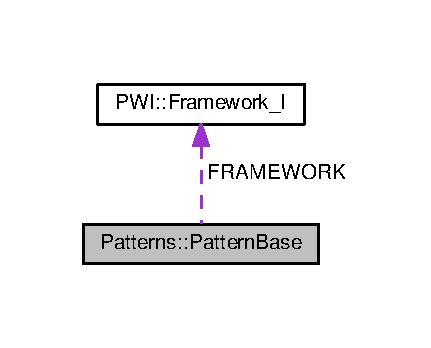
\includegraphics[width=207pt]{apis/class_patterns_1_1_pattern_base__coll__graph}
\end{center}
\end{figure}
\subsection*{Public Member Functions}
\begin{DoxyCompactItemize}
\item 
{\bfseries Pattern\+Base} (\hyperlink{namespace_core_1_1_naming_ab40d44ea919ec3e3c8cc05576ba6d610}{Pattern\+TypeE} type, char \+\_\+unique\+Name\mbox{[}128\mbox{]})\hypertarget{class_patterns_1_1_pattern_base_a994d3c33772d78e35ce2fac5f8913f33}{}\label{class_patterns_1_1_pattern_base_a994d3c33772d78e35ce2fac5f8913f33}

\item 
virtual bool \hyperlink{class_patterns_1_1_pattern_base_a4d36988129317f0e32de31ba0ed7982e}{Start} ()=0\hypertarget{class_patterns_1_1_pattern_base_a4d36988129317f0e32de31ba0ed7982e}{}\label{class_patterns_1_1_pattern_base_a4d36988129317f0e32de31ba0ed7982e}

\begin{DoxyCompactList}\small\item\em Starts the pattern, must be implemented by each pattern. \end{DoxyCompactList}\item 
virtual bool {\bfseries Stop} ()=0\hypertarget{class_patterns_1_1_pattern_base_a8bc96ad07ff84226659ed35f71619f89}{}\label{class_patterns_1_1_pattern_base_a8bc96ad07ff84226659ed35f71619f89}

\item 
virtual \hyperlink{class_patterns_1_1_pattern_base_a892f5cd6d58d75bb43e73cc38a3b882e}{$\sim$\+Pattern\+Base} ()\hypertarget{class_patterns_1_1_pattern_base_a892f5cd6d58d75bb43e73cc38a3b882e}{}\label{class_patterns_1_1_pattern_base_a892f5cd6d58d75bb43e73cc38a3b882e}

\begin{DoxyCompactList}\small\item\em Virtual destructor. \end{DoxyCompactList}\end{DoxyCompactItemize}
\subsection*{Public Attributes}
\begin{DoxyCompactItemize}
\item 
Recv\+Message\+Delegate\+\_\+t $\ast$ {\bfseries recv\+Delegate}\hypertarget{class_patterns_1_1_pattern_base_a51cc459a516bcf914b9ec91e198bc057}{}\label{class_patterns_1_1_pattern_base_a51cc459a516bcf914b9ec91e198bc057}

\item 
Neighbor\+Delegate $\ast$ {\bfseries nbr\+Delegate}\hypertarget{class_patterns_1_1_pattern_base_a62e4f5844c3b0573b5ef28696d5f4b36}{}\label{class_patterns_1_1_pattern_base_a62e4f5844c3b0573b5ef28696d5f4b36}

\item 
Dataflow\+Delegate\+\_\+t $\ast$ {\bfseries dataflow\+Delegate}\hypertarget{class_patterns_1_1_pattern_base_adbecd83eb5b30fb4df328d2b74949d30}{}\label{class_patterns_1_1_pattern_base_adbecd83eb5b30fb4df328d2b74949d30}

\item 
Control\+Response\+Delegate\+\_\+t $\ast$ {\bfseries control\+Delegate}\hypertarget{class_patterns_1_1_pattern_base_af563c486553ba15d62ea3fbb1bf7948b}{}\label{class_patterns_1_1_pattern_base_af563c486553ba15d62ea3fbb1bf7948b}

\end{DoxyCompactItemize}
\subsection*{Protected Member Functions}
\begin{DoxyCompactItemize}
\item 
virtual void {\bfseries Receive\+Message\+Event} (\hyperlink{class_core_1_1_message_t}{F\+Message\+\_\+t} \&msg)=0\hypertarget{class_patterns_1_1_pattern_base_a8adcc760cd5b3396971fcdcd5cd80bd4}{}\label{class_patterns_1_1_pattern_base_a8adcc760cd5b3396971fcdcd5cd80bd4}

\item 
virtual void {\bfseries Neighbor\+Update\+Event} (\hyperlink{struct_core_1_1_neighbor_update_param}{Neighbor\+Update\+Param} nbr\+Update)=0\hypertarget{class_patterns_1_1_pattern_base_acf80253c9df2790d99835dfb8c3c4544}{}\label{class_patterns_1_1_pattern_base_acf80253c9df2790d99835dfb8c3c4544}

\item 
virtual void {\bfseries Data\+Status\+Event} (\hyperlink{struct_core_1_1_dataflow_1_1_data_status_param}{Data\+Status\+Param} notification)=0\hypertarget{class_patterns_1_1_pattern_base_ae56e132583d61c4ca6df0dbcd761da09}{}\label{class_patterns_1_1_pattern_base_ae56e132583d61c4ca6df0dbcd761da09}

\item 
virtual void {\bfseries Control\+Response\+Event} (\hyperlink{struct_p_w_i_1_1_control_response_param}{Control\+Response\+Param} response)=0\hypertarget{class_patterns_1_1_pattern_base_a06b77e9f4bd2d16bad7afa8832642850}{}\label{class_patterns_1_1_pattern_base_a06b77e9f4bd2d16bad7afa8832642850}

\item 
void {\bfseries Register\+Pattern\+Delegates} (Pattern\+Id\+\_\+t pid, \hyperlink{namespace_core_1_1_naming_ab40d44ea919ec3e3c8cc05576ba6d610}{Pattern\+TypeE} \+\_\+type)\hypertarget{class_patterns_1_1_pattern_base_a9e619e83f88c871e62b3cea084b12d1a}{}\label{class_patterns_1_1_pattern_base_a9e619e83f88c871e62b3cea084b12d1a}

\item 
void {\bfseries Handle\+\_\+\+Register\+Response} (\hyperlink{struct_p_w_i_1_1_control_response_param}{Control\+Response\+Param} response)\hypertarget{class_patterns_1_1_pattern_base_aa834f9cdbc178916878211a6177701fe}{}\label{class_patterns_1_1_pattern_base_aa834f9cdbc178916878211a6177701fe}

\item 
void {\bfseries Random\+Local\+Spray} (Pattern\+Id\+\_\+t pid, \hyperlink{class_core_1_1_message_t}{F\+Message\+\_\+t} \&msg, Spray\+TypeE spraytype, bool israndomselection, \hyperlink{class_patterns_1_1_pattern_neighbor_table_i}{Patterns\+::\+Pattern\+Neighbor\+TableI} \&ptn\+Nbr\+Table, uint16\+\_\+t nonce)\hypertarget{class_patterns_1_1_pattern_base_ae17eb4a43493158ff5f146482041ca90}{}\label{class_patterns_1_1_pattern_base_ae17eb4a43493158ff5f146482041ca90}

\item 
bool {\bfseries Randomly\+Select\+Neighbor} (Neigbor\+Container\+Type \&selected\+Neighbor\+List, \hyperlink{class_patterns_1_1_pattern_neighbor_table_i}{Patterns\+::\+Pattern\+Neighbor\+TableI} \&ptn\+Nbr\+Table, Uniform\+Random\+Int $\ast$rand=N\+U\+LL)\hypertarget{class_patterns_1_1_pattern_base_af63159c86bda47a2492815735826dbab}{}\label{class_patterns_1_1_pattern_base_af63159c86bda47a2492815735826dbab}

\item 
void {\bfseries Send2\+Selected\+Neighbors} (Pattern\+Id\+\_\+t pid, Neigbor\+Container\+Type \&selected\+Neighbor\+List, \hyperlink{class_core_1_1_message_t}{F\+Message\+\_\+t} \&msg, uint16\+\_\+t nonce)\hypertarget{class_patterns_1_1_pattern_base_ac52dc18caa96893bd35d6c68970a5bec}{}\label{class_patterns_1_1_pattern_base_ac52dc18caa96893bd35d6c68970a5bec}

\end{DoxyCompactItemize}
\subsection*{Protected Attributes}
\begin{DoxyCompactItemize}
\item 
char {\bfseries unique\+Name} \mbox{[}128\mbox{]}\hypertarget{class_patterns_1_1_pattern_base_a6cff7cf408b665d720a0d2b82a0db9e8}{}\label{class_patterns_1_1_pattern_base_a6cff7cf408b665d720a0d2b82a0db9e8}

\item 
Pattern\+Id\+\_\+t {\bfseries P\+ID}\hypertarget{class_patterns_1_1_pattern_base_aa623ac5f4137e880067aff2092a8c732}{}\label{class_patterns_1_1_pattern_base_aa623ac5f4137e880067aff2092a8c732}

\item 
\hyperlink{class_p_w_i_1_1_framework___i}{Framework\+\_\+I} $\ast$ {\bfseries F\+R\+A\+M\+E\+W\+O\+RK}\hypertarget{class_patterns_1_1_pattern_base_a88b5eb77647f9e40ea741eaf6390d8bf}{}\label{class_patterns_1_1_pattern_base_a88b5eb77647f9e40ea741eaf6390d8bf}

\item 
bool {\bfseries registered}\hypertarget{class_patterns_1_1_pattern_base_a4305a51ad736ccc47242857352d4fa19}{}\label{class_patterns_1_1_pattern_base_a4305a51ad736ccc47242857352d4fa19}

\item 
Pattern\+Request\+StateE {\bfseries request\+State}\hypertarget{class_patterns_1_1_pattern_base_a93a8305be5ae2773af6e24fc18b5a689}{}\label{class_patterns_1_1_pattern_base_a93a8305be5ae2773af6e24fc18b5a689}

\item 
Pattern\+StateE {\bfseries pattern\+State}\hypertarget{class_patterns_1_1_pattern_base_aea5b5ffd6a1c809aa63fefe37ab79c1c}{}\label{class_patterns_1_1_pattern_base_aea5b5ffd6a1c809aa63fefe37ab79c1c}

\item 
uint32\+\_\+t {\bfseries n\+\_\+\+Expected\+Framework\+Responses}\hypertarget{class_patterns_1_1_pattern_base_a5898c2c8a20f9b949abe14cc85cea048}{}\label{class_patterns_1_1_pattern_base_a5898c2c8a20f9b949abe14cc85cea048}

\end{DoxyCompactItemize}


\subsection{Detailed Description}
Defines the abstract base class for patterns. 

The documentation for this class was generated from the following file\+:\begin{DoxyCompactItemize}
\item 
Tuscarora\+F\+W/\+Include/\+Interfaces/\+Pattern/Pattern\+Base.\+h\end{DoxyCompactItemize}

\section{Pattern Example}

In this section we will work through an example of creating and
testing a pattern in the framework.  Our example will be a gossip-like
protocol.  Gossiping is a class of protocols where a particular network
state is updated in the network using periodic/random continuous
messaging.  Gossip-like protocols can be implemented using either
broadcast mechanisms or unicast mechanisms.  In this
example we will implement a unicast-based Gossip (which is
closer to Tuscarora's design philosophy). The state being kept
up to date is simply an integer number that increases monotonically.
The nodes in the network ``gossip'' with each other to make sure they
have the highest/latest number. The code for this example can be
found in the release in the directories
\FilePath{TuscaroraFW/Src/Pattern/Gossip} and \FilePath{TuscaroraFW/Tests/Patterns/Gossip}.


Let's define some basic primitives for the Gossip pattern; 
then we show how to implement these primitives. 


\begin{enumerate}
\item  The pattern sends a status message to selected neighbors at
  random intervals, with some average period---say, 200ms. It uses a
  uniform random number generator and the events module to achieve
  this.  

\item New discovered neighbors are selected to be notified with the
  next status message.

\item If the status info of a received message is older than the
  stored information, its sender is selected to be notified with the
  next status message.

\item  If no new neighbors were selected to be notified, one neighbor
  is selected randomly from the set of neighbors.

\item The list of selected neighbors is cleared after sending a status
  update.

\item If the packet send to a neighbor fails, that neighbor is
  selected again to be notified with the next status message.
\end{enumerate}

\section{Pattern Overview and Definition} \label{sec:PatternCreation}
%\subsection{Pattern Overview}
Operation of the framework and the patterns are asynchronous.
Pattern issues \TuscConcept{Commands} to the Framework, through the PatternBase \CPPVarName{FRAMEWORK} variable. 
For the responses of these \TuscConcept{Commands} as well as 
changes in the pattern neighborhood, 
changes in the status of the previously send packets, and
incoming packets to the pattern,
the framework generates \TuscConcept{Events} and sends them back to the Patterns. 

It is advised that Patterns derive from \CPPClassName{PatternBase} class, since it helps automating registration and bootstrapping procedures of patterns. However, a pattern writer could choose to implement his Pattern from scratch.
\CPPClassName{PatternBase} also provides standard methods that help registering the pattern with the framework. 
In addition to that, it defines virtual functions, one corresponding to each type of \TuscConcept{Event} generated by the Framework, namely 
\begin{itemize}
 \item \CPPFuncName{ReceiveMessageEvent} for handling message receptions, 
 \item \CPPFuncName{NeighborUpdateEvent} for neighbor notifications, 
 \item \CPPFuncName{DataStatusEvent} for handling data notifications, and 
 \item \CPPFuncName{ControlResponseEvent} for handling control responses
\end{itemize}
These functions should be implemented by patterns derived from the \CPPClassName{PatternBase} class.

The code below shows a simple implementation for our \CPPClassName{Gossip} pattern.  


\begin{lstlisting}[style=boralargefile][label={List:Gossip.h}]
/*
 * Gossip.h
 *
 *  Created on:  March 3, 2015
 *     Authors: Mukundan Sridharan, Bora Karaoglu
 */

#ifndef GOSSIP_H_
#define GOSSIP_H_

#include <Types/BasicTypes.h>
#include <Interfaces/Pattern/PatternBase.h>
#include <Lib/Math/Rand.h>
#include "Lib/PAL/PAL_Lib.h"//include the PAL layer
#include "Lib/DS/AVLBinarySearchTreeT.h"

using namespace PWI;

namespace Patterns {

typedef AVLBSTElement<NodeId_t> GossipNeigborContainerTypeElement;
typedef AVLBST_T<NodeId_t> GossipNeigborContainerType;

class GossipLinkComparator: public LinkComparatorI {
public:
  //GossipLinkComparator();
  bool BetterThan (Core::LinkMetrics& A, Core::LinkMetrics& B){
   return (A.quality > B.quality);
  }
};

class Gossip : public PatternBase{
  uint32_t currentStatusId; //Status of the gossip protocol
  FrameworkAttributes fwAttributes;
  uint32_t nonce;
  //Pattern Specific
  UniformRandomInt *rand; //A random number generator
  Event *randEvent_SendUpdate;	//A pointer for the event class used to send random updates
  Event *randEvent_UpdateVar;	//A pointer for the event class used to update stored information
  EventDelegate *eventDel_SendUpdate;//delegate for the random data send event.
  EventDelegate *eventDel_UpdateVar;//delegate for the random data send event.

  void RandomSendHandler(EventDelegateParam param); //Handler for the event generator used to send random updates
  void UpdateVariableHandler(EventDelegateParam param);  //Handler for the event generator used to update stored information

  PatternNeighborTableI *myNbrHood;
  //GossipLinkComparator *myLinkComparator;

  GossipNeigborContainerType SelectedNeighborList; //Set of selected neighbors to send a status update

  FMessage_t& PrepareStatusUpdate();	//Broadcast your status
  void SendMessage();      //Sends a message to the list of selected neighbors
  
  bool SelectNeighbors(NodeId_t nbr); //Add a neighbor to the set of selected neighbors
  void AdjustSelectedNeighbors(); //Make sure at least one neighbor is selected
  void ClearSelectedNeighborList(); //Clear the list of selected neighbors

  NodeId_t IterateThroughNeighbors(uint16_t table_index);
  bool InitiateProtocol();
  void Handle_AttributeResponse(ControlResponseParam response);
  void Handle_LinkThresholdResponse(ControlResponseParam response);
  void Handle_SelectDataNofiticationResponse(ControlResponseParam response);
public:
  //Common to most patterns

  Gossip();	//constructor
  bool Start();  //Lets the test code or network admin start the pattern
  bool Stop(); //Lets the test code or network admin stop the pattern
  
  void NeighborUpdateEvent (NeighborUpdateParam nbrUpdate);
  void ControlResponseEvent (ControlResponseParam response);
  void DataNotificationEvent (DataNotifierParam notification);
  void ReceiveMessageEvent (FMessage_t& msg);
};

} //end of namespace

#endif //GOSSIP_H_
\end{lstlisting}
\label{List:Gossip.h}

The code below shows the definitions provided by the  \CPPClassName{PatternBase} class.  

\begin{lstlisting}[style=boralargefile][label=List:PatternBase.h]
/*
 * PatternI.h
 *
 * 	Author: Mukundan Sridharan
 * 	This is an abstract base class for patterns to derive and implement, to make it easy for registrating with framework and to start them.
 */

#ifndef PATTERN_BASE_H_
#define PATTERN_BASE_H_

#include <Types/BasicTypes.h>
#include <Types/FrameworkTypes.h>
#include <PAL/Delegate.h>
#include <Interfaces/PWI/Framework_I.h>
#include <Interfaces/Core/PatternNamingI.h>


using namespace PAL;
using namespace PWI;
using namespace PWI::Neighborhood;

namespace Patterns {
  //A enum to keep track of Pattern Framework interaction state;
  enum PatternStateE {
    NO_PID,
    GOT_PID,
    REGISTERED,
    EXECUTING,
    ERROR,
  };
  
  enum PatternRequestStateE {
    NONE_PENDING,
    WAITING_FOR_CONTROL_RESPONSE,
    WAITING_FOR_DATA_RESPONSE
  };
///Defines the abstract base class for patterns
class PatternBase {
protected:
  /*
   * @brief Returns a reference to the Pattern's custom neighbor table
   * 
   * @param patternId Pattern's instance ID.
   * @return PWI::Neighborhood::PatternNeighborTableI&. Reference to the patterns neighborhood table.
  
  virtual PatternNeighborTableI& GetNeighborTable(PatternId_t patternId)  = 0;
  */
  
  
protected:
  PatternId_t PID;
  Framework_I* FRAMEWORK;
  bool registered;
  PatternRequestStateE requestState;
  PatternStateE patternState;
  
  virtual void ReceiveMessageEvent (FMessage_t &msg)=0;
  virtual void NeighborUpdateEvent (NeighborUpdateParam nbrUpdate) =0;
  virtual void DataNotificationEvent (DataNotifierParam notification) =0;
  virtual void ControlResponseEvent (ControlResponseParam response) = 0;
  
  void RegisterPattern(PatternId_t pid, PatternTypeE _type);
  void Handle_PatternIDResponse(ControlResponseParam response);
  void Handle_RegisterResponse(ControlResponseParam response);

  
public:
  RecvMessageDelegate_t *recvDelegate;
  NeighborDelegate *nbrDelegate;
  DataflowDelegate_t *dataflowDelegate;
  ControlResponseDelegate_t *controlDelegate;
  /////////////////// Registration and Instantiation Service ////////////////////
  //PatternBase(PatternTypeE type); 
  PatternBase(PatternTypeE type, char uniqueName[128]);
  ///Starts the pattern, must be implemented by each pattern.
  virtual bool Start()=0;
  virtual bool Stop()=0;

  ///Virtual destructor
  virtual ~PatternBase(){}
};

}//End of namespace

#endif /* PATTERN_BASE_H_ */
\end{lstlisting}

\section{Pattern Flow}

Before going into the implementation details, lets look at the flowchart in \cref{fig:PatternFlowChart} that show how the pattern is initialized and is integrated with the framework. \Cref{fig:PatternFlowChart} is divided into 3 sections corresponding the state of the pattern; \CPPConstant{UNREGISTERED}, \CPPConstant{REGISTERED}, and \CPPConstant{EXECUTING}.

%The framework supports usage of both external and internal naming services for obtaining pattern IDs (PID). 
%Patterns using framework supported naming service get their IDs from the framework with the registration response. 
%Hence, for patterns using internal naming services
%\CPPConstant{UNREGISTERED}, and \CPPConstant{GOT\_PID} states are combined and the pattern state changes from \CPPConstant{NO\_PID} to \CPPConstant{REGISTERED} with the reception of a positive registration response. 
%The \CPPClassName{Gossip}, too, employs framework supported naming service and gets its PID with a registration response.  

\begin{figure}[t]
 \centering
 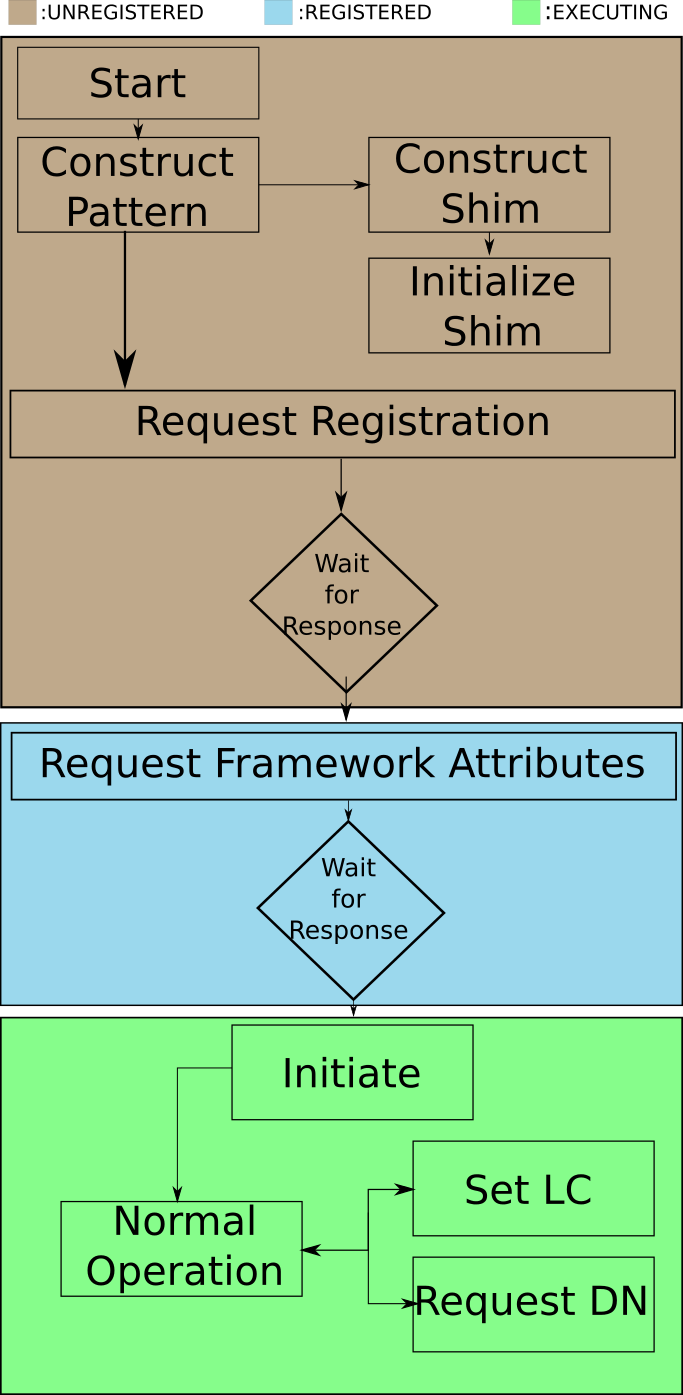
\includegraphics[width=0.4\linewidth]{figures/PatternFlowChart}
 \caption{Flow chart of pattern initialization and registration}
 \label{fig:PatternFlowChart}
\end{figure}



First, the pattern object is constructed. This constructor initializes various parameters of a pattern. 
Next, a shim layer implementing platform specific functions is created. 
Our simple pattern is deriving from \CPPClassName{PatternBase} and call \CPPClassName{PatternBase}'s constructor explicitly that
constructs and initializes the shim layer. 



Initialization of the shim layer 
initializates the internal variables and stores the delegates used for callbacks back to the pattern, namely
\CPPFuncName{ReceiveMessageEvent}, \CPPFuncName{NeighborUpdateEvent},
\CPPFuncName{DataNotificationEvent}, and
\CPPFuncName{ControlResponseEvent}.
However, it does not automatically initiate the registration of the pattern with the framework. \TuscConcept{Patterns} explicitly request registration with the framework and handle framework's response through \CPPFuncName{ControlResponseEvent} function. 

Gossip's PID is assigned by the framework. This PID is included in the positive response to the pattern's registration request,
Receiving a positive response to the pattern's registration request, pattern changes state from \CPPConstant{UNREGISTERED} to \CPPConstant{REGISTERED}. 
At this stage, framework is queried for its attributes. 

By receiving the response to framework attributes request, pattern's state changes to \CPPConstant{EXECUTING}. 
In this state, the pattern initiates its operation and starts operating normally. 
In the beginning of its operation, a pattern can set its link comparator and subscribe to the data notifications of interest. 
However, these operations can be repeated anytime during the normal operation to change the link comparator or to change pattern's subscription to data notifications.  

In the following sections, we will investigate how \CPPClassName{Gossip} implements various functions for its operations.  



\section {Initialization} \label{sec:Initialization}
Patterns deriving from \CPPClassName{PatternBase} initialize their shim layer through \CPPClassName{PatternBase}'s constructor. 
%, which requires a pattern type and a unique string differentiating different instances of the same pattern. 
%\CPPClassName{Gossip}'s constructor further initializes \CPPClassName{Gossip}'s neighborhood by passing criteria for minimum acceptable limits for a link to be accepted in pattern's neighborhood,
%and a comparator for sorting the links to the framework. Next,
%\CPPClassName{Gossip} notifies the framework about the type of
%acknowledgements that it is interested in, namely destination-oriented
%acknowledgments such as a successful (or unsuccessful) reception of
%the packet (indicated by \emph{PDN\_RECV\_DEST\_MASK}), and the acknowledgement
%indicating the availability of the framework to receive packets
%(indicated by \emph{PDN\_WF\_SENT\_MASK}). Finally, \CPPClassName{Gossip} initializes a
%random number generator, two event delegates that are used to schedule
%future events, and the status information to be gossiped.  
\CPPClassName{Gossip}'s constructor further initializes 
\begin{itemize}
	\item two event delegates that are used to schedule
	future events, 
	\item a timer delegate that is used to resend messages in case a message gets lost before getting received by the framework
	\item a random number generator,
	\item a table that stores neighbors,
	\item a nonce and a boolean variables facilitating message passing between the pattern and the framework, and 
	\item internal gossip variables for keeping the status of the gossiped information,
\end{itemize}


\begin{lstlisting}[style=boralargefile][label=List:Gossip.cc:Constructor]
Gossip::Gossip() : PatternBase(Core::Naming::GOSSIP_PTN, (char*)"Gossip_1"){
	Debug_Printf(DBG_PATTERN, "Gossip::Initializing\n");


	//delegate handles to the events
	eventDel_SendUpdate = new EventDelegate(this, &Gossip::RandomSendHandler);
	eventDel_UpdateVar = new EventDelegate(this, &Gossip::UpdateVariableHandler);
	eventDel_ReSendUpdate = new TimerDelegate(this, &Gossip::ReSendHandler);


	//Creates a uniform random number with mean 200,000 and with range +/_100,000
	//That is the values vary between 100,000 to 300,000
	UniformRNGState _state;
	_state.cmrgState.stream = MY_NODE_ID;
	_state.mean = MeanUpdateInterval;
	_state.range = RangeUpdateInterval;
	rand = new UniformRandomInt(_state);

	//Initialize pattern neighbor table
	myNbrHood = new PatternNeighborTable(QUALITY_LC);

	//Initialize variables facilitating message passing
	nonce=1;
	hasFWRejectedPacket = false;

	//Initialize Gossip status
	currentStatusId = 0;
}
\end{lstlisting}

\section {Starting} \label{sec:Starting}

\CPPClassName{Gossip} starts registering itself with the framework with its \CPPFuncName{Start} method. 
In this method, \CPPClassName{Gossip}
initiates pattern registration. 

The framework supports usage of both external and internal naming services for obtaining unique pattern IDs (PID). 
Patterns using framework supported naming service get their IDs from the framework with the registration response while if there is an external service, Pattens can get a PID using this external service prior to registration and include the obtained PID in their registration request. 

Gossip does not have an external pattern naming service and its pattern ID (PID) assigned by the framework during registration. In its registration request, Gossip uses a null \CPPVarName{PID} of 0 together with a unique string identifier of the pattern. The string identifier is used by the framework in generating a \CPPVarName{PID}. 

\begin{lstlisting}[style=boralargefile][label=List:Gossip.cc:Start]
bool Gossip::Start(){
	Debug_Printf(DBG_PATTERN, "Gossip::Start Starting gossiping \n");
	Debug_Printf(DBG_PATTERN, "Gossip:: Sending the RegisterPattern Request to framework...\n");

	FRAMEWORK->RegisterPatternRequest (PID, uniqueName, Core::Naming::GOSSIP_PTN);
	++n_ExpectedFrameworkResponses;
	return true;
}
\end{lstlisting}


\section {Control Response Event Handling} \label{sec:ControlResponseEvent}

The Events related to the control plane are handled by the  \CPPFuncName{ControlResponseEvent} function, which is declared as virtual by the \CPPClassName{PatternBase} class and must be implemented by all patterns deriving from it. 

\CPPClassName{PatternBase} has two internal variables, \CPPVarName{n\_ExpectedFrameworkResponses} and \CPPVarName{patternState}, which help keeping the state of the messaging interface between the patterns and the framework.  

\CPPVarName{patternState} can take values of 
\CPPConstant{NO\_PID},
\CPPConstant{GOT\_PID},
\CPPConstant{REGISTERED}, and
\CPPConstant{EXECUTING}. 
It is updated by a pattern at each stage of the registration process.

%\bk{Again we have to recheck this. how is it moved from \CPPConstant{REGISTERED} to \CPPConstant{EXECUTING} is not clear since it depends on multiple responses. Again, we can use a count instead of absolute state.   }

Patterns expect different responses from the framework depending on their association status. 
%In the case of an unexpected response, \CPPFuncName{ControlResponseEvent} function generates a debug statement. Otherwise, it directs the responses from the framework to the handler functions.
In general, the 
\CPPFuncName{ControlResponseEvent} function implementation should filter out unexpected responses%
\footnote{
An example situation in which an unexpected response might be received from the framework occurs when a pattern crashes and restarts without the crash being detected by the Framework.  
In this case, framework can potentially continue sending responses to earlier requests by the crashed pattern instance.}
and implement error handling for unexpected events from Framework. 

%\bk{We should maybe make the handling of Handle\_RegisterResponse seemsless to the pattern. One method of achieving this could be handling responses with a different funtion at the PatternBase by default and directing it to the Pattern for any response other than PWI::PTN\_RegisterResponse type. }

\begin{itemize}
\item In \CPPConstant{NO\_PID} state, \CPPClassName{Gossip} 
%has just passed its registration request and 
is only expecting a registration response. 
Registration is completed by calling  \CPPClassName{PatternBase}'s \CPPFuncName{Handle\_RegisterResponse}. Next, \CPPClassName{Gossip} queries for the attributes of the framework. 

\item In \CPPConstant{REGISTERED} state, \CPPClassName{Gossip} expects a response to its query for the attributes of the framework. The response for this query is handled in \CPPFuncName{Handle\_AttributeResponse}, which stores the framework attributes and updates \CPPVarName{patternState}.

\item In \CPPConstant{EXECUTING} state, the registration is completed and the pattern is operational. 
In this state the pattern receives responses to various directives that it passes to the framework. 
%Although, there are 6 possible responses in this state, only 
%\CPPConstant{PTN\_SelectDataNotificationResponse}, 
%\\ \CPPConstant{PTN\_SetLinkThresholdResponse}, and 
%\CPPConstant{PTN\_AttributeResponse} 
%are relevant for \CPPClassName{Gossip}. 

	\begin{itemize}
	\item \CPPConstant{PTN\_SelectDataNotificationResponse}: 
	Framework responds to the pattern's selection of data notifications with this response. 
	\CPPClassName{Gossip} handles this response with  \\ \CPPFuncName{Handle\_SelectDataNofiticationResponse}, which checks the success or the failure of the request and generate debug messages. 
	%in addition to updating \CPPVarName{requestState} and \CPPVarName{patternState} variables.
	%\bk{We should handle the case of negative status gracefully. Maybe Start function could be rescheduled attempting to restatr registration procedure.}
	In the case of a failure, \CPPFuncName{The SelectDataNotificationsRequest()} function is called to issue a new request to the framework to set the appropriate data notification masks.
	
	\item \CPPConstant{PTN\_SetLinkThresholdResponse}: 
	Framework responds to the pattern's selection of link threshold with this response. 
	\CPPClassName{Gossip} handles this response with \\ \CPPFuncName{Handle\_LinkThresholdResponse}, which checks the success or the failure of the request and generate debug messages. 
	%in addition to updating \CPPVarName{requestState} and \CPPVarName{patternState} variables.
	%\bk{We should handle the case of negative status gracefully. Maybe a different threshold response is scheduled.}
	In the case of a failure, \CPPFuncName{SetNeighborhoodandLinkComparator()} function is recalled issuing a new request to the framework for link comparator and threshold. 
	
	\item \CPPConstant{PTN\_AttributeResponse}: 
	This is a notification indicates some change in framework's attributes. \CPPClassName{Gossip} handles this response with \CPPFuncName{Handle\_AttributeResponse} function similar to the \CPPConstant{REGISTERED} state.
	
	\item \CPPConstant{PTN\_AddDestinationResponse}: 
	This is the framework's response to a request to add a destination(s) to the list of destinations of a previous packet before it is sent out of the waveform.   
	Not used by \CPPClassName{Gossip}.
	
	\item \CPPConstant{PTN\_ReplacePayloadResponse}: 
	This is the framework's response to a request to replace the payload of a previous packet before it is sent out of the waveform.   
	Not used by \CPPClassName{Gossip}.
	
	\item \CPPConstant{PTN\_CancelDataResponse}: 
	This is the framework's response to a request to stop one of its previous packets before it is sent out of the waveform.  
	Not used by \CPPClassName{Gossip}.
	
	
	\end{itemize}

\end{itemize}


\begin{lstlisting}[style=boralargefile] [label=List:Gossip.cc:ControlResponseEvent]
void Gossip::ControlResponseEvent(ControlResponseParam response)
{
	Debug_Printf(DBG_PATTERN, "Gossip:: Got a control response of type %d\n", response.type);
	switch (patternState){
	case NO_PID:
	case GOT_PID:
		if(response.type == PWI::PTN_RegisterResponse){
    		--n_ExpectedFrameworkResponses;
			Handle_RegisterResponse(response);
			FRAMEWORK->FrameworkAttributesRequest(PID);
			++n_ExpectedFrameworkResponses;
		}else {
			Debug_Printf(DBG_PATTERN, "Gossip:: ControlResponseEvent: My state is %d I got wrong response type %d\n", patternState, response.type);
		}
		break;
	case REGISTERED:
		if(response.type == PWI::PTN_AttributeResponse){
    		--n_ExpectedFrameworkResponses;
    		Handle_AttributeResponse(response);
    		InitiateProtocol();

		}else {
			Debug_Printf(DBG_PATTERN, "Gossip:: ControlResponseEvent: My state is %d, I got wrong response type %d\n", patternState,response.type);
		}
		break;
	case EXECUTING:
		switch(response.type){
		case PTN_SelectDataNotificationResponse:
            Handle_SelectDataNofiticationResponse(response);
            --n_ExpectedFrameworkResponses;
			break;
		case PTN_SetLinkThresholdResponse:
			Handle_LinkThresholdResponse(response);
			--n_ExpectedFrameworkResponses;
			break;
		case PTN_AttributeResponse:
    		--n_ExpectedFrameworkResponses;
    		Handle_AttributeResponse(response);
    		InitiateProtocol();
    		break;
		case PTN_AddDestinationResponse:
		case PTN_ReplacePayloadResponse:
		case PTN_CancelDataResponse:
		default:
			Debug_Printf(DBG_PATTERN, "Gossip:: ControlResponseEvent: My state is %d, I got wrong response type %d\n", patternState,response.type);
			break;
		}
		break;
		default:
			break;
	}
}


void Gossip::Handle_AttributeResponse(ControlResponseParam response){
	FrameworkAttributes *atr = (FrameworkAttributes*) response.data;
	fwAttributes = *atr;

	if( patternState == REGISTERED) {
		patternState = EXECUTING;
	}
	else {
		 Debug_Printf(DBG_PATTERN, "PatternBase::Pattern getting initiated without registration.\n");
	}

	Debug_Printf(DBG_PATTERN,"Gossip:: Handle_AttributeResponse: Framework supports %d waveforms, with max pkt size is %d .\n", fwAttributes.numberOfWaveforms, fwAttributes.maxFrameworkPacketSize);
	for(uint i=0; i<fwAttributes.numberOfWaveforms; i++){
		Debug_Printf(DBG_PATTERN, "Gossip::Handle_AttributeResponse: Waveform %d Id is %d\n", i, fwAttributes.waveformIds[i]);
	}
}
\end{lstlisting}

\section {Initiation} \label{sec:Initiation}

With the reception of a positive response to its registration request, \CPPClassName{Gossip} initiates its operation with \CPPFuncName{InitiateProtocol()} function.

In this function, \CPPClassName{Gossip} calls \CPPFuncName{SetNeighborhoodandLinkComparator()} to select
%Patterns select 
(i) a link comparator type defining the criteria for differentiating between links, and 
(ii) a threshold defining minimum acceptable limits for a link to be accepted in pattern's neighborhood. 
%Both the comparator and the threshold are passed to the framework. 
\CPPClassName{Gossip} selects the link quality as the criterion to differentiate between links and sets its threshold to a quality level of 0.1. 

Next, by calling \CPPFuncName{RequestDataNotifications()} function,
\CPPClassName{Gossip} notifies the framework about the type of acknowledgements that it is interested in, 
namely destination-oriented acknowledgments 
such as a successful (or unsuccessful) reception of the packet (indicated by \CPPConstant{PDN\_RECV\_DEST\_MASK}).
%and the acknowledgement indicating the availability of the framework to receive packets (indicated by \CPPConstant{PDN\_WF\_SENT\_MASK}).


%These settings finalize \CPPClassName{Gossip}'s configuration and 
Finally, \CPPClassName{Gossip} initiates its operation by starting two random event generators used for (i) periodically sending messages and updating the
information (see the next section). 
These random event generators are stopped in \CPPClassName{Gossip}'s stop routine, which stops the operation of the pattern. 

%Finally, a timer, \CPPVarName{randEvent\_ReSendUpdate}, is initialized. This timer is rescheduled when a data message is sent and is used for resending message to the framework if a response is not received for a \CPPVarName{ReSendTimeOutInterval}.  

\begin{lstlisting}[style=boralargefile][label=List:Gossip.cc:InitiateProtocol]
bool Gossip::InitiateProtocol(){
	//Initialize neighborhood and set link comparator.
	SetNeighborhoodandLinkComparator();

	//tell framework which notifications you are interested in
	RequestDataNotifications();

	Debug_Printf(DBG_PATTERN, "Gossip::Have configured everything succeessfully. Good to go. \n");

	uint64_t eventDelay = rand->GetNext();
	//The event callback will have null parameter
	randEvent_SendUpdate = new Event(eventDelay, *eventDel_SendUpdate, (void *) 0);
	randEvent_UpdateVar = new Event(eventDelay, *eventDel_UpdateVar, (void *) 0);

	randEvent_ReSendUpdate = new Timer(ReSendTimeOutInterval, ONE_SHOT, *eventDel_ReSendUpdate);
	randEvent_ReSendUpdate->Suspend();
	return true;
}

void Gossip::SetNeighborhoodandLinkComparator(){
	FRAMEWORK->SelectLinkComparatorRequest(PID,PWI::Neighborhood::QUALITY_LC);
	++n_ExpectedFrameworkResponses;
	//FRAMEWORK->SelectLinkComparatorRequest (PID, QUALITY_LC);
	LinkMetrics myThreshold;
	myThreshold.quality = 0.10;


	FRAMEWORK->SetLinkThresholdRequest(PID,myThreshold);
	requestState = WAITING_FOR_CONTROL_RESPONSE;
	++n_ExpectedFrameworkResponses;
}

void Gossip::RequestDataNotifications(){
	uint8_t mask = PDN_RECV_DEST_MASK;
	FRAMEWORK->SelectDataNotificationRequest(PID, mask);
	requestState = WAITING_FOR_CONTROL_RESPONSE;
	++n_ExpectedFrameworkResponses;
}
\end{lstlisting}


\section {Data Status Handling} \label{sec:DataNotificationEvent}

Packet related notifications are handled with \CPPFuncName{DataStatusEvent(DataStatusParam ntfy)}. 
The patterns notify the framework about the type of notifications that they are interested in. They can change this request anytime throughout the course of operation. For a full list of notifications please refer to the TuscaroraFramework\_API documentation.

In its start routine, \CPPClassName{Gossip} passes its interest on two types of acknowledgements: 
\begin{itemize}
\item \CPPConstant{PDN\_RECV\_DEST\_MASK}: Since \CPPClassName{Gossip} registers for this type, it will be notified about
whether a packet was successfully received via a \CPPClassName{DataNotifierParam} with a \CPPVarName{ackType} of \CPPConstant{PDN\_DST\_RECV}. 
%Each notification includes information about \CPPVarName{ntfy.noOfDest} listed in the array \CPPVarName{ntfy.dest[]}. 
\CPPVarName{ntfy.status} indicates the success or the failure of the reception by the \CPPVarName{ntfy.noOfDest} destinations listed in the array, \CPPVarName{ntfy.dest[]}.
For negative acknowledgements, \CPPClassName{Gossip} adds the list of negatively acknowledged destinations into its list of neighbors to be updated in the next cycle. 

%\bk{The source code is modified to include the suggested changes. It should be rechecked before the release }

\item \CPPConstant{PDN\_FW\_RECV\_MASK}: This notification type is on by default for all patterns and is generated without requiring to ask for it. Framework notifies \CPPClassName{Gossip} whether it accepts the previous packet sent by the pattern via a \CPPClassName{DataNotifierParam} with a \CPPVarName{ackType} of \CPPConstant{PDN\_FW\_RECV}. \CPPVarName{ntfy.status} indicates whether the packet is accepted or rejected. 
With the reception of the response, \CPPClassName{Gossip} 
cancels the timer that resends packets after a timeout period after which no response is received. 
For accepted packets, \CPPClassName{Gossip} further clears the list of selected neighbors, and increments \CPPVarName{nonce} variable used to identify packets not yet assigned a packet id.
For rejected packets, \CPPClassName{Gossip} further checks \CPPVarName{ntfy.readyToReceive} parameter that indicate whether the framework is accepting new packets at that moment and resends a status update with the same \CPPVarName{nonce} id if it does. 
On the other hand, if the framework indicates that it is not ready to accept packets, \CPPClassName{Gossip} sets the \CPPVarName{hasFWRejectedPacket} variable preserving the state. 
In that state, \CPPClassName{Gossip} tries sending a new status update%
\footnote{but with the same nonce id since it is not matched to any messages yet}
with the reception of a future data notification (of any \CPPVarName{ackType}) that indicates the availability of the framework to receive packets.   

\end{itemize}

\begin{lstlisting}[style=boralargefile] [label=List:Gossip.cc:ReceiveDataNotifications]
void Gossip::ReceiveDataNotifications(DataNotifierParam ntfy) {
	///You have received ack for previous message.
	//check what happened to the previous message
	Debug_Printf(DBG_PATTERN,"Gossip:: Received a data notification from framework\n");
	switch (ntfy.type){
		case ACK_DST_RECV:
			if(!ntfy.status ){
				Debug_Printf(DBG_PATTERN,"Gossip:: Message id %d not received by destination\n", ntfy.messageId);
				SelectNeighbors(ntfy.dest);
			}
		break;
		case READY_TO_RECV:
			SendMessage();
		break;
		default:
		break;
	}
}
\end{lstlisting}

\section {Neighbor Updates} \label{sec:NeighborUpdateEvent}
Neighbor related notifications are handled by
\CPPFuncName{NeighborUpdateEvent(NeighborUpdateParam nbrUpdate)}, which
is defined as virtual by the \CPPClassName{PatternBase} and must be implemented by all patterns deriving from it. 
%In the registration process with the framework, \CPPClassName{PatternBase} class defines this function as the target for the neighbor update events. 

For each change in the pattern neighborhood, the framework notifies the pattern with a \CPPVarName{NeighborUpdateParam} that has a \CPPVarName{changeType} of  
\begin{itemize}
\item \CPPVarName{NBR\_NEW} for detected links, 
\item \CPPVarName{NBR\_DEAD} for links that are detected as broken or not satisfying the threshold conditions specified,
\item \CPPVarName{NBR\_UPDATE} for links that remain in neighborhood but change some properties.
\end{itemize}
%(i)~links that are discovered and links that are detected with an \CPPVarName{nbrUpdate.changeType} of \emph{NBR\_NEW}, 
%(ii)~links that aredetected as broken or not satisfying the threshold conditions specified with an \emph{nbrUpdate.changeType} of \emph{NBR\_DEAD},
%(iii)~links that remain in neighborhood but change some propertieswith an \emph{nbrUpdate.changeType} of \emph{NBR\_UPDATE}.  
\CPPClassName{Gossip} uses the \CPPFuncName{UpdateTable(NeighborUpdateParam \_param)} of the \CPPClassName{PatternNeighborTable} to make the corresponding changes in the \CPPVarName{myNbrHood}.

\begin{lstlisting}[style=boralargefile][label=List:Gossip.cc:NeighborUpdateEvent]
void Gossip::NeighborUpdateEvent(NeighborUpdateParam nbrUpdate)
{
  myNbrHood->UpdateTable(nbrUpdate);
}
void Patterns::PatternNeighborTable::UpdateTable(NeighborUpdateParam _param)
{
	//bool signalPattern=false;
	LinkMap *newLink;Link *ptnLink;
	switch(_param.changeType)
	{
	case NBR_NEW:
		newLink = new LinkMap(_param.link.linkId, _param.link);
		nbrhood->Insert(newLink);
		//signalPattern =true;
		break;
	case NBR_DEAD:
		if(nbrhood->DeleteLink(_param.link.linkId)){
			//signalPattern =true;
		}
		break;
	case NBR_UPDATE:
		Debug_Printf(DBG_PATTERN, "PatternNeighborTable:: updating neighbor %d on waveform %d\n", _param.nodeId, _param.link.linkId.waveformId);fflush (stdout);
		ptnLink = nbrhood->GetLink(_param.link.linkId);
		if(ptnLink){
			if(ptnLink->linkId.waveformId){
				ptnLink->metrics = _param.link.metrics;
			}
		}else {
			printf("Mismatch in neighbor table status, I (Pattern %d) dont have link (%d, %d) in table, but received an update event \n Created new link\n",
					this->patternId,_param.nodeId, _param.link.linkId.waveformId);
			newLink = new LinkMap(_param.link.linkId, _param.link);
			nbrhood->Insert(newLink);
		}

		break;
	default:
		printf("PatternNeighborTable:: Error: wrong neighbor update signal\n");
		break;
	}
}
\end{lstlisting}

\section {Receiving Messages} \label{sec:ReceiveMessageEvent}

Received messages are handled by \CPPFuncName{ReceiveMessage(FMessage\_t\& msg)}. 
In this function, \CPPClassName{Gossip} compares the status ID reported in the packet with the internal state ID. If the internal state variable (\CPPVarName{currentStatusId})
\begin{itemize} 
\item  is smaller than the one reported in the packet, the internal state variable is updated. 
\item is larger than the one reported in the packet, the source node of the the packet is added to the list of nodes that will be reported in the following period.  
\item is equal to the one reported in the packet, the packet is ignored. 
\end{itemize}  
% XXXXXXXXX KC sez:  I think the ">=" in the following should be "<".
% According to the problem statement above, our state should be the
% highest/latest ID.
% BK: You are right. We should update if the message's status is larger/newer than the internal one.
\begin{lstlisting}[style=boralargefile] [label=List:Gossip.cc:ReceiveMessageEvent]
void Gossip::ReceiveMessageEvent(FMessage_t& msg)
{
  GossipMsg* gMsg = (GossipMsg*) msg.GetPayload();
 Debug_Printf(DBG_PATTERN, "Gossip:: Received msg from %u with status seq %u \n",msg.GetSource(), gMsg->currentStatusId);
  //Process the recevied message
  if(currentStatusId < gMsg->currentStatusId) {
	  currentStatusId = gMsg->currentStatusId;
  }
  else if(currentStatusId > gMsg->currentStatusId) {
	  SelectNeighbors(msg.GetSource());
  }
}
\end{lstlisting}

\section {Handling Scheduled Events} \label{sec:ScheduledEvents}

Next, we implement the handler methods of scheduled events. 
In \CPPClassName{Gossip}, we have two such methods: a method that periodically
sends messages, \CPPFuncName{RandomSendHandler(EventDelegateParam param)}; 
and a method that increments the state of the pattern,
\emph{UpdateVariableHandler(EventDelegateParam param)}. 
Both of these methods are scheduled randomly and reschedule their triggering events when executed. 
When sending an update, if no nodes were selected before, we randomly
select a node using \emph{AdjustSelectedNeighbors()}. 
We make sure
that the selected node is a neighbor and was not already selected
using \emph{SelectNeighbors(NodeId\_t nbr)}.

\begin{lstlisting}[style=boralargefile] [label=List:Gossip.cc:RandomSendHandler]
//Handler for the randEvent_UpdateVar event
void Gossip::UpdateVariableHandler(EventDelegateParam param){
	uint64_t eventDelay = rand->GetNext();
	uint64_t curTime = Debug::GetTimeMicro();
	param.eventPtr->ReSchedule(eventDelay*100,(void *) (0));
	Debug_Printf(DBG_PATTERN, "UpdateVariable:: Rescheduled event to fire at %lu\n",curTime+eventDelay);
	++currentStatusId;
}
//Handler for the RandomSend event
void Gossip::RandomSendHandler(EventDelegateParam param){
  //Lets us first reshedule the event
  uint64_t eventDelay = rand->GetNext();
  uint64_t curTime = Debug::GetTimeMicro();
  param.eventPtr->ReSchedule(eventDelay,(void *) (0));
 Debug_Printf(DBG_PATTERN,"Gossip::RandomSend:: Rescheduled event to fire at %lu\n",curTime+eventDelay);fflush(stdout);
  //Now lets broadcast our status
  AdjustSelectedNeighbors();
  if(SelectedNeighborList.Size() > 0) SendMessage(); //If I have at least one destination send this message
}

void Gossip::AdjustSelectedNeighbors() {
	if(SelectedNeighborList.Size() > 0) return; //Already selected neighbors based on other criteria
	uint16_t nbrCount = myNbrHood->GetNumberOfNeighbors();
	Debug_Printf(DBG_PATTERN,"Gossip:: Got %d neighbors  \n", nbrCount);fflush(stdout);
	if (nbrCount == 0) return;//Return if there are no neighbors to choose from
	NodeId_t sNeighbor;
	uint16_t i=0;
	while(SelectedNeighborList.Size() == 0) {
		uint64_t pickrandom = rand->GetNext();
		pickrandom = pickrandom % nbrCount;
		Debug_Printf(DBG_PATTERN,"Gossip:: Got %d neighbors and picking %lu neighbor from tabel  \n", nbrCount, pickrandom);fflush(stdout);
		PatternNeighborIterator it = myNbrHood->Begin();
		for(uint16_t ii=0; ii< nbrCount; ii++) {
			if(pickrandom == 0) {	
				sNeighbor = (it->linkId.nodeId);
			}
			--pickrandom;
			Debug_Printf(DBG_PATTERN,"Gossip:: Intering neighbortable inde %d neighbor is %d \n",ii, it->linkId.nodeId);fflush(stdout);
			it=it.GetNext();
		}
		/*if(pickrandom == 0) {
			sNeighbor = (it->linkId.nodeId);
		}*/
	      
		
		Debug_Printf(DBG_PATTERN,"Gossip:: Selected %d neighbor \n", sNeighbor);fflush(stdout);
		if( SelectNeighbors(sNeighbor) ) {
			Debug_Printf(DBG_PATTERN,"Gossip:: PickRandomNeighbor %d \n", sNeighbor);fflush(stdout);
		}
		i++;
		Debug_Printf(DBG_PATTERN,"Gossip:: in while %d times  \n", i);fflush(stdout);
	}
}

bool Gossip::SelectNeighbors(NodeId_t nbr){
	if( myNbrHood->GetNeighborLink(nbr) && !(SelectedNeighborList.Search(nbr)) ) { //If the node is my neighbor and not selected before
		Debug_Printf(DBG_PATTERN,"Gossip:: SelectNeighbor: Ading neighbor %d neighbors  to SelectedNeighborList \n", nbr);fflush(stdout);
		return SelectedNeighborList.Insert(nbr);
	}
	return false;
}
}
\end{lstlisting}

\section {Sending Messages} \label{sec:SendingMessages}

Sending status update messages is implemented in
\CPPFuncName{SendMessage()}. 
This method creates a packet containing the
current status information of the node using
\CPPFuncName{PrepareStatusUpdate()}, 
and passes the constructed packet to the framework
along with 
\begin{itemize}
\item an array including the set of previously selected destinations in \CPPVarName{SelectedNeighborList},
\item the size of this array,
\item a temporary pattern generated message ID, namely \CPPVarName{nonce} and
\item a boolen variable indicating whether ACKs are requested. 
\end{itemize}

While sending a message to the framework, pattern should provide a temporary ID to the message called a \CPPVarName{nonce}, which is used to identify a packet until a unique Message ID is generated for the message by the Framework and returned to the Pattern. 
When the framework receives the packet, it generates a \CPPVarName{DataNotifierParam} with an \CPPVarName{ackType} of \CPPConstant{PDN\_WF\_RECV}.  
This \CPPVarName{DataNotifierParam} also includes the \CPPVarName{nonce} generated with the pattern along with the \CPPVarName{messageId} that can be used to uniquely identify the message from that point on.

The nonce is also useful for error detection and recovery, if either the Command from pattern to framework gets lost or if the Data Notification Event with the message ID from the framework gets lost. A pattern in general should start a timer when sending a message to the framework and if a Data Notification for the message is not received before the timer expires, it should resend the same message with the same nonce. If the framework receives two consecutive messages with the same nonce, it would recognize it as a duplicate and resend the data notification for that packet. 
 

\CPPFuncName{SendMessage()} function also schedules an event resending a new packet if no framework response is received in \CPPConstant{ReSendTimeOutInterval}. 
Finally, the \CPPVarName{hasFWRejectedPacket} state variable is cleared since the packet has not been rejected at that time instant. 
This state variable can be set via a data notification as discussed in \cref{sec:DataNotificationEvent}.

%If the framework rejects the message, \emph{SendMessage()} terminates and is re-invoked when the framework later notifies the pattern that it is free to accept messages. If the framework accepts the packet, \emph{SelectedNeighborList} is cleared.
\begin{lstlisting}[style=boralargefile] [label=List:Gossip.cc:SendMessage]
// This function broadcast status
FMessage_t& Gossip::PrepareStatusUpdate(){
	Debug_Printf(DBG_PATTERN, "Gossip:: PrepareStatusUpdate\n");
	
	//Construct packet and send
	FMessage_t *sendMsg;
	//Make sure to use new() operator to create packet on heap.
	sendMsg = new FMessage_t(sizeof(struct GossipMsg));
	sendMsg->SetSource(MY_NODE_ID);
	sendMsg->SetInstance(PID);
	
	GossipMsg* gMsg = (GossipMsg*) sendMsg->GetPayload();
	gMsg->currentStatusId=currentStatusId;
	return (*sendMsg);
}
// This function sends a message to the list of selected neighbors
void Gossip::SendMessage() {
	NodeId_t selnodes[SelectedNeighborList.Size()];
	GossipNeigborContainerTypeElement* elptr = SelectedNeighborList.Begin();
	int i=0;
	while(elptr){
		selnodes[i] = elptr->data;
		elptr = SelectedNeighborList.Next(elptr);
		++i;
	}
	Debug_Printf(DBG_PATTERN, "Gossip::SendMessage multicasting to %d destinations \n", SelectedNeighborList.Size()); fflush(stdout);
	MessageId_t msgID = FRAMEWORK->Send(selnodes, (uint16_t) SelectedNeighborList.Size(), PrepareStatusUpdate(), (U64NanoTime*) NULL, false);
	
	if (msgID == 0){
		Debug_Printf(DBG_PATTERN, "Gossip::SendMessage framework is busy. Rejected the packet. Keeping list of neighbors.\n"); fflush(stdout);
	}
	else{
		Debug_Printf(DBG_PATTERN, "Gossip::SendMessage framework accepted message (%d). \n", msgID);fflush(stdout);
		ClearSelectedNeighborList();
	}
}

void Gossip::ClearSelectedNeighborList(){
	GossipNeigborContainerTypeElement *elptr,*elptr2;
	elptr = SelectedNeighborList.Begin();
	while(SelectedNeighborList.Size()>0){
		elptr2 = SelectedNeighborList.Next(elptr);
		SelectedNeighborList.DeleteElement(elptr);
		elptr = elptr2;
	}
}
\end{lstlisting}

\section {Broadcasting a Message } \label{sec:BroadcastingMessages}

While \CPPClassName{Gossip} primarily uses generic \CPPFuncName{SendData} API, sending a broadcast message is quite similar. The primary
difference is that, 
while generic \CPPFuncName{SendData} primitive addresses to one or more destinations, 
a broadcast is addressed to a particular waveform.
The framework uses the waveform's broadcast API (if it has one) to
send the message. 
\textit{Please note that how the actual broadcasting is
  implemented is up to the waveform provider.} 
The other difference is that a broadcast message will not generate any \CPPConstant{PDN\_DST\_RECV} data notifications, 
but will generate the \CPPConstant{PDN\_FW\_RECV} when the message is accepted by the framework, and 
\CPPConstant{PDN\_WF\_SENT} when the waveform has sent the message out.
The number of waveforms available on a node and their IDs are obtained by the Pattern using the \CPPFuncName{FrameworkAttributeRequest()} Command issued while the pattern initialized. 
Once their IDs are known, the waveform IDs can be used to send broadcasts. 
The code listing belows shows an example of sending a broadcast message.

\begin{lstlisting}[style=boralargefile]  [label=List::BroadcastMessage]
///These lines show how to handle AttributeResponse to parse and get the waveform IDs
void Gossip::Handle_AttributeResponse(ControlResponseParam response){
	FrameworkAttributes *atr = (FrameworkAttributes*) response.data;
	fwAttributes = *atr;
	requestState = NONE_PENDING;
	patternState = EXECUTING;
	active=true;
	Debug_Printf(DBG_PATTERN,"FWP:: Handle_AttributeResponse: Framework supports %d waveforms, with max pkt size is %d .\n", fwAttributes.numberOfWaveforms, fwAttributes.maxFrameworkPacketSize);
	for(uint i=0; i<fwAttributes.numberOfWaveforms; i++){
		Debug_Printf(DBG_PATTERN, "FWP::Handle_AttributeResponse: Waveform %d Id is %d\n", i, fwAttributes.waveformIds[i]);
	}
}


///Creating and sending broadcast
FMessage_t *sendMsg = new FMessage_t();
sendMsg->SetType(Types::Pattern_Type);
sendMsg->SetInstance(PID);
sendMsg->SetPayload(&dataPtr[i*maxPayload]); //Set some payload
sendMsg->SetPayloadSize(maxPayload); //Set payload size

///Send a broadcast on the first waveform
FRAMEWORK->BroadcastData(PID, *sendMsg, fwAttributes.waveformIds[0] , nonce);
\end{lstlisting}

\section {Stopping}
The \CPPClassName{Gossip} stops its operation when its \CPPFuncName{Stop} method is called. 
If there are previously scheduled events for 
sending updates, 
updating internal gossip value, and 
resending an update after a predefined value,
this method cancels them. 
This in turn also stops rescheduling of these events. 
\begin{lstlisting}[style=boralargefile][label=List:Gossip.cc:Stop]
bool Gossip::Stop()
{
	randEvent_UpdateVar->Cancel();
	randEvent_SendUpdate->Cancel();
	randEvent_ReSendUpdate->Suspend();
	return true;
}
\end{lstlisting}

\section {Testing the Pattern}

In order to test the pattern, a separate test needs to be written.
The test code is separate so that the pattern
code can be used for simulation, deployment, and across
different hardware platforms. The tests reside under the
\FilePath{Tuscarora/Tests/} directory.  Pattern tests reside under
\FilePath{Tuscarora/Tests/Patterns/<pattern-name>} directory. In our
case the test files can be found under \FilePath{Tuscarora/Tests/Patterns/Gossip}.

The runOrDebug script in the Tuscarora root directory finds all the
tests under the \FilePath{Tuscarora/Tests} directory and compile them. 
The test files have the format \FilePath{run<TestModuleName>.cpp}. 
To run a test, you need to simply provide the \FilePath{<TestModuleName>} 
corresponding to the test file,
%which has the format \FilePath{run<TestModuleName>.cpp}, 
which in our case is ``Gossip''. 
Each test has a
``main'' method, which first sets the node id, instantiates the framework
modules, and finally creates an instance of the specific test and
executes the test.

\begin{lstlisting}[style=boralargefile] [label=List:runGossip.cpp:main]
//main for the test
int main(int argc, char* argv[]) {
  //Make sure RuntimeOpts construction is the very first line of main
  RuntimeOpts opts ( argc-1, argv+1 );
  
  MY_NODE_ID = atoi(getenv("NODEID"));
 // NETWORK_SIZE = opts.nodes;
   //Turn on debugging for Gossip pattern
//   DBG_TEST = true;
 // set in Lib/Misc/Debug.cpp
//   DBG_PATTERN = true;
 // set in Lib/Misc/Debug.cpp
//   //DBG_WAVEFORM = true;
 // set in Lib/Misc/Debug.cpp
//   //DBG_CORE_DATAFLOW = true;
 // set in Lib/Misc/Debug.cpp

//   DBG_CORE = true;
 // set in Lib/Misc/Debug.cpp

  FW_Init fwInit;
  fwInit.InitFI();
  fwInit.Execute(&opts);
  
  GossipTest *gossipTest = new GossipTest();
  gossipTest->Execute(&opts);

  while(1){sleep(1);}
  return 0;
}
\end{lstlisting}

The \emph{GossipTest} class itself is quite simple and exposes an
Execute method, which is used to start the test. 
The constructor and the Execute method of this class are used to setup and
start the test respectively. 
The \emph{GossipTest} starts a 2-second timer to let the network stabilize. (This example also shows how to initialize and use a timer module). The timer is started within the Execute method and when the timer fires, the Gossip pattern is started. 

\begin{lstlisting}[style=boralargefile] [label=List:runGossip.cpp:GossipTest]
GossipTest::GossipTest(){
	//Turn on debugging for Gossip pattern
// 	DBG_PATTERN = true;
 // set in Lib/Misc/Debug.cpp
// 	DBG_WAVEFORM = false;
 // set in Lib/Misc/Debug.cpp
// 	DBG_CORE = false;
 // set in Lib/Misc/Debug.cpp
	
	PatternId_t pid = GetNewPatternInstanceId(Gossip_P);
	gossip = new Gossip(pid);
	timerDel = new TimerDelegate (this, &GossipTest::TimerHandler);
	startTestTimer = new Timer(2000000, ONE_SHOT, *timerDel);
	}
	
	void GossipTest::TimerHandler(uint32_t event){
	Debug_Printf(DBG_PATTERN, "GossipTEST: Starting the Gossip Pattern...\n");
	gossip->Start();
	}
	
	void GossipTest::Execute(RuntimeOpts *opts){
	//Delay starting the actual pattern, to let the network stabilize
	//So start the timer now and when timer expires start the pattern
	Debug_Printf(DBG_PATTERN,"About to start timer on node 1\n");
	startTestTimer->Start();
}
\end{lstlisting}






\chapter{Waveform Development}
\label{Chap:Waveform}
%\section{Waveform Interface}

This chapter explains some of the features of the waveform interface. The interface is defined in a flexible way to accommodate a diverse set of waveforms. 

\section{Overview}

The waveform interface serves as the lower interface of the Tuscarora Framework.  Any waveform that satisfies the interface definition may be plugged into the Framework for use alongside other waveforms, in order to support a heterogeneous MANET.

To satisfy the waveform interface, a waveform provider needs to implement a single interface, called \CPPClassName{Waveform\_I}.  The interface, \CPPClassName{Waveform\_I} is a template class that is instantiated by passing the waveform’s address type as a template parameter.  In total, there are 10 methods in each instantiated class, of which 3 are optional, that is, a waveform provider can choose to not implement any or all of the optional methods. \cref{Fig:WaveformModules} shows the waveform
interfaces as related to the framework interfaces.


\begin{figure}[h]
 \centering
 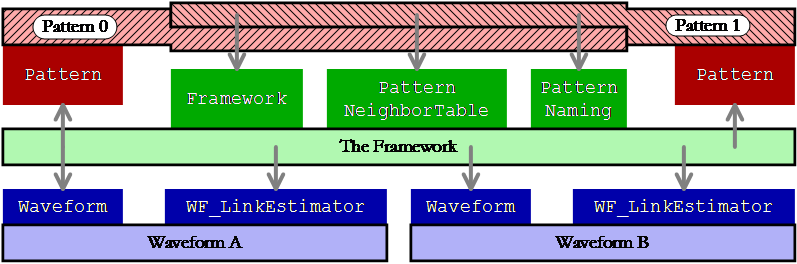
\includegraphics[width=0.9\linewidth]{figures/WaveformModules}
 \caption{Waveform Interfaces}
 \label{Fig:WaveformModules}
\end{figure}

Please refer to the Framework API documentation for full detail about the \CPPClassName{Waveform\_I} interface. 


\subsection {Programming Style:  Syntax and Semantics}
The interface design uses asynchronous message passing semantics, with a functional syntax, to define interactions between the waveform and Tuscarora.  It consists of two sorts of methods:  1) incoming commands, exercised by the user of the interface (namely, the Framework, via a communication shim) on the waveform, and 2) outgoing events, sent by the waveform to the user of the interface.

In terms of syntax, both commands and events are specified using function calls.  This simple representation yields ease of programming and, equally importantly, avoids restriction to a particular implementation of method invocation, such as socket communications between processes, which may be appropriate for some use cases (e.g., on large hardware platforms) but not others (e.g., for ns-3 simulation platforms where the overhead seems to matter).

In terms of semantics, all interface methods are explicitly associated with a message passing semantics.  The message passing semantics is reflected by the fact that all incoming commands have a return type of void.  Moreover, for any command that expects some sort of response from the waveform, an associated event method exists in the waveform interface, to convey the result of the computation.

The design assumes that a communication library, which we colloquially refer to as a “shim-layer”, is provided that implements the invocation of command and event methods using asynchronous message  passing.  The slightly different shim layer might be required for each waveform-platform pair, although generally far fewer shim layers would be required.

\subsection {Data Plane and Control Plane}
The waveform interface functionality spans a Data Plane and a Control Plane.  The Data Plan interface consists of the functions SendData, BroadcastData, Data Notification Event and the Received Message Event.  The remaining commands and events, as detailed below, which deal with the control status of the waveform, link estimation and schedules comprise the Control Plane. Figure 1 shows the Summary of the Commands and the Events that are expected by the framework in response to them, split across the Data and Control planes. The dotted lines show the dependency between a command and the event. 

\subsection {Interface Interaction Pattern using Asynchronous Message Passing}
In general, the data and control plane functions follow a common interaction pattern.  A command originates from Tuscarora to the waveform and, subsequently, one or more corresponding events are sent from the waveform back to the Framework.  Events are mapped and routed to particular modules and/or function within the Framework; it is convenient to think of each event as “named pipe” between the waveform and the Framework.  Each event is specified as a class with a single “Invoke” method that has a specific type of parameter. The Invoke method returns a bool (as against the void return type of most commands). The return type of Invoke indicates the status of queuing the Event on to the communication mechanism. The return type does not indicate the success or failure of sending the event to the framework. For example, if an Invoke returned a ‘true’ it means that the shim layer responsible for the communication has accepted the event and has queued it up for sending at a latter time. If it returns a ‘false’, it means either the communication mechanism is either broken or is busy processing existing events and cannot accept any new events to be sent out.
Five types of events are defined for the waveform:
\begin{enumerate}
\item Received Message Event (WF\_RcvMessageEvent\_t):  This Event is sent whenever a data message is received on the waveform, with WF\_RecvMsgParam  as the parameter.
\item	Data Notification Event (WF\_DataNotifierEvent\_t):  This Event is sent to convey the status of the SendData and BroadcastData calls and the WF\_DataNotifierParam is used as the event parameter. This Event might be generated up to three times for each data message, once to acknowledge the message has been received by the waveform, once when it is sent out and once when the message is received at the destination.
\item	Control Response Event (WF\_ControlResponseEvent\_t):  This Event is sent in response to one of the request commands in the control plane with WF\_ControlRssponseParam as the parameter. The parameter contains a response type, response status (success/failure), any additional data and its size.
\item	Link Estimation Event (WF\_LinkEstimateEvent\_t):  This Event is sent to provide to the Framework link estimates updates about a neighbor. The WF\_LinkEventParam is used as the parameter for this event.
\item	Schedule Update Event (WF\_ScheduleUpdateEvent\_t):  This Event is sent by the waveform to provide updates about its sending or receiving schedules. WF\_ScheduleUpdateParam is used as the event parameter.
\end{enumerate}

Every command originating from the Framework has a sequence number and the events use the same sequence number to identify their response.  The Framework tracks the sequence number it uses for each command and if it fails to receive a response for some command, it may resend that command with the same sequence number.  The waveform using the same sequence number to send multiple response to the same command or to update/change the response to the command is acceptable.  For the control plane commands the sequence number is called as the “RequestId”, for the data plane it is called as the “MessageId”.  A couple of special cases are allowed:  The Link Estimation Event and the Schedule Update Event do not use sequence numbers in their events and error recovery is not provided for those events.  For the Received Message Event the sequence number is generated by the Waveform and sent to the Framework.

\subsection {Control Plane State}

As far as the Framework’s awareness of the control state of the waveform is concerned, it knows only that the state of the waveform can be one of the following states which are defined by the enum WF\_ControlP\_StatusE:
\begin{itemize}
	\item WF\_NORMAL:  Waveform has been initialized and is operating within “normal” bounds.
	\item WF\_BUSY:  Waveform has been initialized, but is busy with non-data plane functions. The Framework should desist from sending messages to waveform, it is likely that the waveform might not accept the messages.
	\item WF\_ERROR:  Waveform is in an error state. The Framework should not send messages to waveform, until the status changes.
	\item WF\_BUFFER\_LOW:  The waveform is operating normally, but is at risk of running out of messages to send out. The Framework may respond by attempting to increase the data output to the waveform.
	\item WF\_BUFFER\_FULL:  The waveform is operating normally, but is at risk of being overrun by data packets. The Framework should respond by slow down its rate of invoking data packet sends on the waveform.
\end{itemize}


\subsection {Flow Control}
The Waveform accomplishes flow control between the Waveform and Framework in one of three ways:

\begin{enumerate}
	\item	Waveform can drop the packet being sent to it and return a negative status when sending a data notification message back to the Framework.  The Framework will interpret this as the waveform not being ready to receive data messages.
	\item	Waveform can send a WF\_BUFFER\_LOW or WF\_BUFFER\_FULL response messages to the Framework, to request it to speed up or slow down the data message rate.
	\item	Waveform can send a WF\_ERROR status message to completely stop receiving any data messages from the Framework if it has to clear a backlog.  It could subsequently send a WF\_NORMAL status message when it is ready to resume.
	The remaining sections describe the API methods (first commands, then events) in detail.
\end{enumerate}

\subsection {Parameter Ownership}
In Tuscarora whenever a function call happens across layers the ownership of the data structures passed as parameters is transferred to the callee. In this particular case, this applies to the commands the Waveform\_I interface receives and the event calls the waveform makes. We call the “Give” model of ownership where the ownership is given when to the callee. The Give model is used to avoid deep copying of packets and other parameters at the callee so that efficiency of processing can be improved. However, there are some implications of this “Give” model. 
\begin{itemize}
\item Pass by reference: Any large parameter objects should be passed by reference in a function to make optimum use of the Give model. Passing by value does not utilize the Give model. However, for small objects this might not matter much.

\item Allocation on heap: The caller must also be explicitly aware of which parameters are passed as references, since these objects must be allocated on the heap (and not on the local stack). Creating a local object and passing this as reference to another method will result in run time errors. Also, once a parameter has been passed as reference and the call has been made, the same object cannot be modified by the caller anymore. This would also result in run time errors.

\item Deallocation:  It is the callee’s responsibility to deallocate any parameter that is  passed by reference, since these were originally allocated on the heap by the caller. Failing to deallocate (or reuse) such objects will result in a memory leak. 
\end{itemize}



\section{Packet Metadata}

Waveforms should also provide metadata for each packet received.
The metadata provided is standardized across all
waveforms. Currently 3 types of metadata have been defined, (i)
Received signal strength indicator (RSSI), (ii) Signal to noise and
interference ratio (SINR) and (iii) Packet reception time stamp.
The metadata is used by the framework to create and/or improve the
estimates for the properties of links.
%estimates of the the neighbors.

\if false
\begin{lstlisting}[style=boralargefile][captionpos=b,caption={Waveform attributes structure used to expose information about the waveform to framework},label=List:Attributes]
 
struct WaveformAttributes{
  uint16_t wfId;		///Waveform Ids given by the framework
  WF_TypeE type;		///Type of waveform	
  WF_EstimatorTypeE estType;	///Type of estimator provided by the waveform
  WF_AntennaTypeE antType;	///Type of antenna used by the waveform
  WF_ModeE mode;		///Current mode of the waveform
  uint16_t ifindex;		///Waveform OS/Platform interfce index number
  char name[32];		///Name of waveform
  uint16_t headerSize;		///Size of the waveform header in bytes
  uint16_t maxPayloadSize;	///Maximum payload that can be sent on the waveform in 			bytes
  uint16_t maxPacketSize;	///Maximum packet size that can be sent on the waveform 			(in bytes), including the waveform header
  uint16_t minPacketSize;	///Minimum packet size that can be sent on the waveform 			(in bytes), including the waveform header
  uint32_t minInterPacketDelay; ///Minimum interpacket rate in micro seconds
  uint32_t channelRate; 	///The channel rate in bytes per second
  uint32_t maxBurstRate; 	///Maximum data burst rate in bytes per second
};
\end{lstlisting}

\fi

%\hypertarget{class_waveform_1_1_waveform_base}{}\section{Waveform\+:\+:Waveform\+Base Class Reference}
\label{class_waveform_1_1_waveform_base}\index{Waveform\+::\+Waveform\+Base@{Waveform\+::\+Waveform\+Base}}


Inheritance diagram for Waveform\+:\+:Waveform\+Base\+:\nopagebreak
\begin{figure}[H]
\begin{center}
\leavevmode
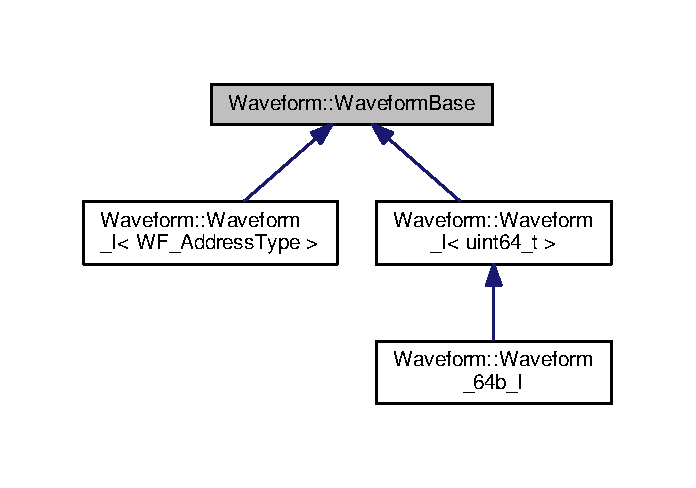
\includegraphics[width=334pt]{class_waveform_1_1_waveform_base__inherit__graph}
\end{center}
\end{figure}
\subsection*{Public Member Functions}
\begin{DoxyCompactItemize}
\item 
virtual void \hyperlink{class_waveform_1_1_waveform_base_a67053c3a29b7fa3f477dce71a15fc624}{Replace\+Payload\+Request} (Request\+Id\+\_\+t r\+Id, W\+F\+\_\+\+Message\+Id\+\_\+t msg\+Id, uint8\+\_\+t $\ast$payload, uint16\+\_\+t payload\+Size)=0
\begin{DoxyCompactList}\small\item\em Requests the replacement the payload of a message, passed in an earlier call to ‘\+Send\+Data’ or ‘\+Broadcast\+Data’ method with the given Message\+Id. The previous payload will be discarded. \end{DoxyCompactList}\item 
virtual void \hyperlink{class_waveform_1_1_waveform_base_aad9cfbc04a5168caa1780edd812d6f7d}{Attributes\+Request} (Request\+Id\+\_\+t r\+Id)=0
\begin{DoxyCompactList}\small\item\em Request the attributes of the waveform. \end{DoxyCompactList}\item 
virtual void \hyperlink{class_waveform_1_1_waveform_base_ac5a64312ea70923af969c51cc4e0363d}{Control\+Status\+Request} (Request\+Id\+\_\+t r\+Id)=0
\begin{DoxyCompactList}\small\item\em Requests the control status of waveform. A W\+F\+\_\+\+StatusE enum type is sent as the data of the response message, to indicate the status of the variable. \end{DoxyCompactList}\item 
virtual void \hyperlink{class_waveform_1_1_waveform_base_a767db0e1d92d0e3ae46da3b2335e9b87}{Data\+Status\+Request} (Request\+Id\+\_\+t r\+Id, W\+F\+\_\+\+Message\+Id\+\_\+t m\+Id)=0
\begin{DoxyCompactList}\small\item\em Requests the status of a data message already sent to the waveform. \end{DoxyCompactList}\item 
virtual void \hyperlink{class_waveform_1_1_waveform_base_ad0e6f375f176315332c7e90d57fb8a21}{Set\+Schedule\+Request} (Request\+Id\+\_\+t r\+Id, Node\+Id\+\_\+t node\+Id, W\+F\+\_\+\+Schedule\+TypeE type, Schedule\+BaseI \&schedule, uint16\+\_\+t schedule\+Size)
\begin{DoxyCompactList}\small\item\em Sends information about a schedule for one of 3 kinds of functions\+: link estmation, sending or receiving to the waveform. \end{DoxyCompactList}\item 
virtual void {\bfseries Schedule\+Request} (Request\+Id\+\_\+t r\+Id, Node\+Id\+\_\+t nodeid, W\+F\+\_\+\+Schedule\+TypeE type)\hypertarget{class_waveform_1_1_waveform_base_ac443d02d12315ac2aeb4cb0f62c35862}{}\label{class_waveform_1_1_waveform_base_ac443d02d12315ac2aeb4cb0f62c35862}

\end{DoxyCompactItemize}


\subsection{Member Function Documentation}
\index{Waveform\+::\+Waveform\+Base@{Waveform\+::\+Waveform\+Base}!Attributes\+Request@{Attributes\+Request}}
\index{Attributes\+Request@{Attributes\+Request}!Waveform\+::\+Waveform\+Base@{Waveform\+::\+Waveform\+Base}}
\subsubsection[{\texorpdfstring{Attributes\+Request(\+Request\+Id\+\_\+t r\+Id)=0}{AttributesRequest(RequestId_t rId)=0}}]{\setlength{\rightskip}{0pt plus 5cm}virtual void Waveform\+::\+Waveform\+Base\+::\+Attributes\+Request (
\begin{DoxyParamCaption}
\item[{Request\+Id\+\_\+t}]{r\+Id}
\end{DoxyParamCaption}
)\hspace{0.3cm}{\ttfamily [pure virtual]}}\hypertarget{class_waveform_1_1_waveform_base_aad9cfbc04a5168caa1780edd812d6f7d}{}\label{class_waveform_1_1_waveform_base_aad9cfbc04a5168caa1780edd812d6f7d}


Request the attributes of the waveform. 

{\bfseries Semantic Behavior\+:} \hyperlink{namespace_waveform}{Waveform} should return its attributes to the Framework by generating a response through the Control Response Event, with the same request ID. The status of the response message should be true, unless otherwise the attributes are not available to be sent to the Framework. The response contains attributes in the \hyperlink{struct_waveform_1_1_w_f___attributes}{W\+F\+\_\+\+Attributes} structure, which is copied into the data portion of the \hyperlink{struct_waveform_1_1_w_f___control_response_param}{W\+F\+\_\+\+Control\+Response\+Param}.


\begin{DoxyParams}{Parameters}
{\em r\+Id} & Specifies the ID of the request, which the waveform will use to in its response message. \\
\hline
\end{DoxyParams}
\begin{DoxyReturn}{Returns}
void. 
\end{DoxyReturn}


Implemented in \hyperlink{class_waveform_1_1_waveform__64b___i_a11e3bb3d2db8b8f1f7f63159782af9ce}{Waveform\+::\+Waveform\+\_\+64b\+\_\+I}.

\index{Waveform\+::\+Waveform\+Base@{Waveform\+::\+Waveform\+Base}!Control\+Status\+Request@{Control\+Status\+Request}}
\index{Control\+Status\+Request@{Control\+Status\+Request}!Waveform\+::\+Waveform\+Base@{Waveform\+::\+Waveform\+Base}}
\subsubsection[{\texorpdfstring{Control\+Status\+Request(\+Request\+Id\+\_\+t r\+Id)=0}{ControlStatusRequest(RequestId_t rId)=0}}]{\setlength{\rightskip}{0pt plus 5cm}virtual void Waveform\+::\+Waveform\+Base\+::\+Control\+Status\+Request (
\begin{DoxyParamCaption}
\item[{Request\+Id\+\_\+t}]{r\+Id}
\end{DoxyParamCaption}
)\hspace{0.3cm}{\ttfamily [pure virtual]}}\hypertarget{class_waveform_1_1_waveform_base_ac5a64312ea70923af969c51cc4e0363d}{}\label{class_waveform_1_1_waveform_base_ac5a64312ea70923af969c51cc4e0363d}


Requests the control status of waveform. A W\+F\+\_\+\+StatusE enum type is sent as the data of the response message, to indicate the status of the variable. 

{\bfseries Semantic Behavior\+:} The Framework expects the waveform to be in one of the data plane states defined by the W\+F\+\_\+\+Control\+P\+\_\+\+StatusE enum. The waveform should return the current status of its data plane by generating a response through the Control Response Event, with the same Request\+Id. The status that response message should be true. The actual data plane status should be copied into the data part of the response


\begin{DoxyParams}{Parameters}
{\em r\+Id} & Specifies the ID of the request, which the waveform will use to in its response message. \\
\hline
\end{DoxyParams}
\begin{DoxyReturn}{Returns}
void. 
\end{DoxyReturn}


Implemented in \hyperlink{class_waveform_1_1_waveform__64b___i_ae13e7e49359ea2e45b010cdf4f1d3227}{Waveform\+::\+Waveform\+\_\+64b\+\_\+I}.

\index{Waveform\+::\+Waveform\+Base@{Waveform\+::\+Waveform\+Base}!Data\+Status\+Request@{Data\+Status\+Request}}
\index{Data\+Status\+Request@{Data\+Status\+Request}!Waveform\+::\+Waveform\+Base@{Waveform\+::\+Waveform\+Base}}
\subsubsection[{\texorpdfstring{Data\+Status\+Request(\+Request\+Id\+\_\+t r\+Id, W\+F\+\_\+\+Message\+Id\+\_\+t m\+Id)=0}{DataStatusRequest(RequestId_t rId, WF_MessageId_t mId)=0}}]{\setlength{\rightskip}{0pt plus 5cm}virtual void Waveform\+::\+Waveform\+Base\+::\+Data\+Status\+Request (
\begin{DoxyParamCaption}
\item[{Request\+Id\+\_\+t}]{r\+Id, }
\item[{W\+F\+\_\+\+Message\+Id\+\_\+t}]{m\+Id}
\end{DoxyParamCaption}
)\hspace{0.3cm}{\ttfamily [pure virtual]}}\hypertarget{class_waveform_1_1_waveform_base_a767db0e1d92d0e3ae46da3b2335e9b87}{}\label{class_waveform_1_1_waveform_base_a767db0e1d92d0e3ae46da3b2335e9b87}


Requests the status of a data message already sent to the waveform. 

{\bfseries Semantic Behavior\+:} If the Framework is uncertain about the status of a message that it sent to the waveform, it can send the Data\+Status\+Request command. A response message should be generated through the Control Response Event, with the same Request\+Id, that should have the status set as ‘true’ if the waveform received the particular message and a W\+F\+\_\+\+Data\+Notifier\+Param object must be created that reflects the current status of the message and should be copied into the data part of the \hyperlink{struct_waveform_1_1_w_f___control_response_param}{W\+F\+\_\+\+Control\+Response\+Param}.


\begin{DoxyParams}{Parameters}
{\em r\+Id} & Specifies the ID of the request, which the waveform will use to in its response message. \\
\hline
{\em m\+Id} & Specified the ID of the message, for which status is requested. \\
\hline
\end{DoxyParams}
\begin{DoxyReturn}{Returns}
void. 
\end{DoxyReturn}


Implemented in \hyperlink{class_waveform_1_1_waveform__64b___i_a06bcaf416cc353850232ee373b3bac01}{Waveform\+::\+Waveform\+\_\+64b\+\_\+I}.

\index{Waveform\+::\+Waveform\+Base@{Waveform\+::\+Waveform\+Base}!Replace\+Payload\+Request@{Replace\+Payload\+Request}}
\index{Replace\+Payload\+Request@{Replace\+Payload\+Request}!Waveform\+::\+Waveform\+Base@{Waveform\+::\+Waveform\+Base}}
\subsubsection[{\texorpdfstring{Replace\+Payload\+Request(\+Request\+Id\+\_\+t r\+Id, W\+F\+\_\+\+Message\+Id\+\_\+t msg\+Id, uint8\+\_\+t $\ast$payload, uint16\+\_\+t payload\+Size)=0}{ReplacePayloadRequest(RequestId_t rId, WF_MessageId_t msgId, uint8_t *payload, uint16_t payloadSize)=0}}]{\setlength{\rightskip}{0pt plus 5cm}virtual void Waveform\+::\+Waveform\+Base\+::\+Replace\+Payload\+Request (
\begin{DoxyParamCaption}
\item[{Request\+Id\+\_\+t}]{r\+Id, }
\item[{W\+F\+\_\+\+Message\+Id\+\_\+t}]{msg\+Id, }
\item[{uint8\+\_\+t $\ast$}]{payload, }
\item[{uint16\+\_\+t}]{payload\+Size}
\end{DoxyParamCaption}
)\hspace{0.3cm}{\ttfamily [pure virtual]}}\hypertarget{class_waveform_1_1_waveform_base_a67053c3a29b7fa3f477dce71a15fc624}{}\label{class_waveform_1_1_waveform_base_a67053c3a29b7fa3f477dce71a15fc624}


Requests the replacement the payload of a message, passed in an earlier call to ‘\+Send\+Data’ or ‘\+Broadcast\+Data’ method with the given Message\+Id. The previous payload will be discarded. 

{\bfseries Semantic Behavior\+:} \hyperlink{namespace_waveform}{Waveform} should replace the payload of a message passed in an earlier call to ‘\+Send\+Data’ or ‘\+Broadcast\+Data’ method with the given message ID, if the message has not been sent out. A response message should be generated through the Control Response Event, with the same request ID, that should include a status which will be set to false if the message has been sent out or if the waveform is unable to replace the payload of a message. Otherwise, the status should be set to true in the response message.


\begin{DoxyParams}{Parameters}
{\em r\+Id} & Specifies the ID of the request, which the waveform will use to in its response message. \\
\hline
{\em msg\+Id} & specifies the message ID of the packet. \\
\hline
{\em payload} & pointer to the new payload. \\
\hline
{\em payload\+Size} & size of the new payload. \\
\hline
\end{DoxyParams}
\begin{DoxyReturn}{Returns}
void. 
\end{DoxyReturn}


Implemented in \hyperlink{class_waveform_1_1_waveform__64b___i_a90bdc9d75233d1453c486ad200126b90}{Waveform\+::\+Waveform\+\_\+64b\+\_\+I}.

\index{Waveform\+::\+Waveform\+Base@{Waveform\+::\+Waveform\+Base}!Set\+Schedule\+Request@{Set\+Schedule\+Request}}
\index{Set\+Schedule\+Request@{Set\+Schedule\+Request}!Waveform\+::\+Waveform\+Base@{Waveform\+::\+Waveform\+Base}}
\subsubsection[{\texorpdfstring{Set\+Schedule\+Request(\+Request\+Id\+\_\+t r\+Id, Node\+Id\+\_\+t node\+Id, W\+F\+\_\+\+Schedule\+Type\+E type, Schedule\+Base\+I \&schedule, uint16\+\_\+t schedule\+Size)}{SetScheduleRequest(RequestId_t rId, NodeId_t nodeId, WF_ScheduleTypeE type, ScheduleBaseI &schedule, uint16_t scheduleSize)}}]{\setlength{\rightskip}{0pt plus 5cm}virtual void Waveform\+::\+Waveform\+Base\+::\+Set\+Schedule\+Request (
\begin{DoxyParamCaption}
\item[{Request\+Id\+\_\+t}]{r\+Id, }
\item[{Node\+Id\+\_\+t}]{node\+Id, }
\item[{W\+F\+\_\+\+Schedule\+TypeE}]{type, }
\item[{Schedule\+BaseI \&}]{schedule, }
\item[{uint16\+\_\+t}]{schedule\+Size}
\end{DoxyParamCaption}
)\hspace{0.3cm}{\ttfamily [inline]}, {\ttfamily [virtual]}}\hypertarget{class_waveform_1_1_waveform_base_ad0e6f375f176315332c7e90d57fb8a21}{}\label{class_waveform_1_1_waveform_base_ad0e6f375f176315332c7e90d57fb8a21}


Sends information about a schedule for one of 3 kinds of functions\+: link estmation, sending or receiving to the waveform. 

{\bfseries Semantic Behavior\+:} This method enables the Framework to pass on some scheduling information to the waveform. The expectation is that this method will be implemented only if the waveform needs scheduling information from the Framework or an external third party provider. The method enables receiving scheduling information specific to a neighbor specified by the \+\_\+node\+Id parameter. The schedule information is sent as abstract schedule object represented by the \+\_\+schedule object and the size of this object is specified by the \+\_\+schedule\+Size parameter. The expectation is that, if a waveform needs scheduling information, it will derive from the Schedule\+BaseI class and will implement its own scheduling class. The Framework defines three types of waveform schedules as the W\+F\+\_\+\+Schedule\+TypeE enum (one each for link estimation, sending, and receiving messages).

The waveform should regenerate a response to this request through the Control Response Event, with the same Request\+Id. The status of that response message should be true if the waveform able to successfully use the scheduler information or false otherwise.

Since this is an optional feature for waveforms, if it choose to implement it, the waveform should set the scheduler\+Info\+Support field in its Attribute as true whenever it responds to the Attribute\+Request.


\begin{DoxyParams}{Parameters}
{\em r\+Id} & Specifies the ID of the request, which the waveform will use to in its response message. \\
\hline
{\em nodeid} & Specifies the node ID for which the schedule should be used. \\
\hline
{\em type} & Enum that specifies the type of the schedule. There are 3 types of schedules, sending, receiving and link estimation. \\
\hline
{\em schedule} & Reference to an abstract schedule object. It is expected that this class will be derived and implemented by different waveforms. \\
\hline
{\em schedule\+Size} & Size of the schedule object. \\
\hline
\end{DoxyParams}
\begin{DoxyReturn}{Returns}
void. 
\end{DoxyReturn}


The documentation for this class was generated from the following file\+:\begin{DoxyCompactItemize}
\item 
Tuscarora\+F\+W/\+Include/\+Interfaces/\+Waveform/W\+F\+\_\+\+I.\+h\end{DoxyCompactItemize}



%\hypertarget{class_waveform_1_1_waveform___i}{}\section{Waveform\+:\+:Waveform\+\_\+I$<$ W\+F\+\_\+\+Address\+Type $>$ Class Template Reference}
\label{class_waveform_1_1_waveform___i}\index{Waveform\+::\+Waveform\+\_\+\+I$<$ W\+F\+\_\+\+Address\+Type $>$@{Waveform\+::\+Waveform\+\_\+\+I$<$ W\+F\+\_\+\+Address\+Type $>$}}


Defines the generic iteractions for waveforms.  




{\ttfamily \#include $<$W\+F\+\_\+\+I.\+h$>$}



Inheritance diagram for Waveform\+:\+:Waveform\+\_\+I$<$ W\+F\+\_\+\+Address\+Type $>$\+:\nopagebreak
\begin{figure}[H]
\begin{center}
\leavevmode
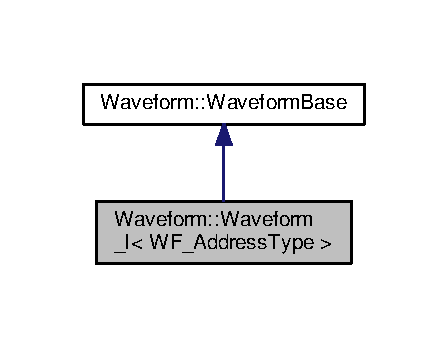
\includegraphics[width=215pt]{class_waveform_1_1_waveform___i__inherit__graph}
\end{center}
\end{figure}


Collaboration diagram for Waveform\+:\+:Waveform\+\_\+I$<$ W\+F\+\_\+\+Address\+Type $>$\+:\nopagebreak
\begin{figure}[H]
\begin{center}
\leavevmode
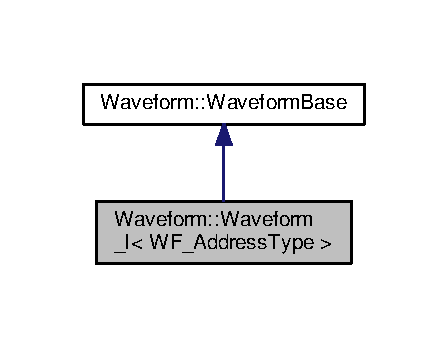
\includegraphics[width=215pt]{class_waveform_1_1_waveform___i__coll__graph}
\end{center}
\end{figure}
\subsection*{Public Types}
\begin{DoxyCompactItemize}
\item 
typedef \hyperlink{class_waveform_1_1_w_f___event}{W\+F\+\_\+\+Event}$<$ W\+F\+\_\+\+R\+E\+C\+V\+\_\+\+M\+S\+G\+\_\+\+E\+VT, \hyperlink{struct_waveform_1_1_w_f___recv_msg_param}{W\+F\+\_\+\+Recv\+Msg\+Param}$<$ W\+F\+\_\+\+Address\+Type $>$ $>$ {\bfseries W\+F\+\_\+\+Rcv\+Message\+Event\+\_\+t}\hypertarget{class_waveform_1_1_waveform___i_ac3fb531925a9157639bf197fee7e8418}{}\label{class_waveform_1_1_waveform___i_ac3fb531925a9157639bf197fee7e8418}

\item 
typedef \hyperlink{class_waveform_1_1_w_f___event}{W\+F\+\_\+\+Event}$<$ W\+F\+\_\+\+D\+A\+T\+A\+\_\+\+N\+T\+Y\+\_\+\+E\+VT, \hyperlink{struct_waveform_1_1_w_f___data_status_param}{W\+F\+\_\+\+Data\+Status\+Param}$<$ W\+F\+\_\+\+Address\+Type $>$ $>$ {\bfseries W\+F\+\_\+\+Data\+Status\+Event\+\_\+t}\hypertarget{class_waveform_1_1_waveform___i_a5efbb2428b3d0dbe51994f70a352a1ba}{}\label{class_waveform_1_1_waveform___i_a5efbb2428b3d0dbe51994f70a352a1ba}

\item 
typedef \hyperlink{class_waveform_1_1_w_f___event}{W\+F\+\_\+\+Event}$<$ W\+F\+\_\+\+L\+I\+N\+K\+\_\+\+E\+S\+T\+\_\+\+E\+VT, \hyperlink{struct_core_1_1_w_f___link_estimation_param}{W\+F\+\_\+\+Link\+Estimation\+Param}$<$ W\+F\+\_\+\+Address\+Type $>$ $>$ {\bfseries W\+F\+\_\+\+Link\+Estimate\+Event\+\_\+t}\hypertarget{class_waveform_1_1_waveform___i_a90a5d0b20f5e152b91d3e9701c9db069}{}\label{class_waveform_1_1_waveform___i_a90a5d0b20f5e152b91d3e9701c9db069}

\end{DoxyCompactItemize}
\subsection*{Public Member Functions}
\begin{DoxyCompactItemize}
\item 
\hyperlink{class_waveform_1_1_waveform___i_a98959d954f80b314ef896d2f857b7e4c}{Waveform\+\_\+I} (Waveform\+Id\+\_\+t \+\_\+w\+Id, \hyperlink{namespace_waveform_a8362d1abeefedecd1142a174faedc096}{W\+F\+\_\+\+TypeE} \+\_\+type, \hyperlink{namespace_waveform_a264307e95d31e27c5a69031fd2615f98}{W\+F\+\_\+\+Estimator\+TypeE} \+\_\+est\+Type, char $\ast$\+\_\+device\+Name)
\begin{DoxyCompactList}\small\item\em Constructor. Creates a waveform object. \end{DoxyCompactList}\item 
virtual void \hyperlink{class_waveform_1_1_waveform___i_ab651687e82a54481718d2ee75e40ec53}{Send\+Data} (\hyperlink{class_waveform_1_1_w_f___message_t}{W\+F\+\_\+\+MessageT}$<$ W\+F\+\_\+\+Address\+Type $>$ \&\+\_\+msg, uint16\+\_\+t \+\_\+payload\+Size, W\+F\+\_\+\+Address\+Type $\ast$\+\_\+dest\+Array, uint16\+\_\+t \+\_\+no\+Of\+Dest, W\+F\+\_\+\+Message\+Id\+\_\+t \+\_\+msg\+Id, bool \+\_\+no\+Ack=false)=0
\begin{DoxyCompactList}\small\item\em Send message indicated by the Message\+Id to a set of neighbors indicated by dest\+Array, with a given payload size. \end{DoxyCompactList}\item 
virtual void \hyperlink{class_waveform_1_1_waveform___i_ac2ddb96d5fb3c8cd410f688acde95389}{Broadcast\+Data} (\hyperlink{class_waveform_1_1_w_f___message_t}{W\+F\+\_\+\+MessageT}$<$ W\+F\+\_\+\+Address\+Type $>$ \&\+\_\+msg, uint16\+\_\+t \+\_\+payload\+Size, W\+F\+\_\+\+Message\+Id\+\_\+t \+\_\+msg\+Id)
\begin{DoxyCompactList}\small\item\em Sends a broadcast on a waveform. Destination received data notification will not be generated If the waveform does not support physical layer broadcasting, the implementation is upto the waveform or the waveform might simply not implement this interface. \end{DoxyCompactList}\item 
virtual void \hyperlink{class_waveform_1_1_waveform___i_a0dc200e92cdff86e55d65ab270c988e6}{Cancel\+Data\+Request} (Request\+Id\+\_\+t \+\_\+r\+Id, W\+F\+\_\+\+Message\+Id\+\_\+t \+\_\+msg\+Id, W\+F\+\_\+\+Address\+Type $\ast$\+\_\+dest\+Array, uint16\+\_\+t \+\_\+no\+Of\+Destinations)=0
\begin{DoxyCompactList}\small\item\em Requests the Cancellation of a data message already sent to the waveform for one or more destinations. \end{DoxyCompactList}\item 
virtual void \hyperlink{class_waveform_1_1_waveform___i_ace837715041bdea1e7857ccd9858e3f2}{Add\+Destination\+Request} (Request\+Id\+\_\+t \+\_\+r\+Id, W\+F\+\_\+\+Message\+Id\+\_\+t \+\_\+msg\+Id, W\+F\+\_\+\+Address\+Type $\ast$\+\_\+dest\+Array, uint16\+\_\+t \+\_\+no\+Of\+Destinations)=0
\begin{DoxyCompactList}\small\item\em Adds one or more destinations to a packet, that has already been sent to the waveform. \hyperlink{namespace_waveform}{Waveform} will send a Control Response Event as reply to this command. \end{DoxyCompactList}\item 
virtual \hyperlink{class_waveform_1_1_waveform___i_a1f0f3d3a86e5b34ca19d84a5425ea7ba}{$\sim$\+Waveform\+\_\+I} ()\hypertarget{class_waveform_1_1_waveform___i_a1f0f3d3a86e5b34ca19d84a5425ea7ba}{}\label{class_waveform_1_1_waveform___i_a1f0f3d3a86e5b34ca19d84a5425ea7ba}

\begin{DoxyCompactList}\small\item\em virtual destructor for interface \end{DoxyCompactList}\end{DoxyCompactItemize}
\subsection*{Protected Attributes}
\begin{DoxyCompactItemize}
\item 
Waveform\+Id\+\_\+t {\bfseries W\+ID}\hypertarget{class_waveform_1_1_waveform___i_af7ee22c008f34e6ba23a8fe00f3db901}{}\label{class_waveform_1_1_waveform___i_af7ee22c008f34e6ba23a8fe00f3db901}

\item 
\hyperlink{namespace_waveform_a8362d1abeefedecd1142a174faedc096}{W\+F\+\_\+\+TypeE} {\bfseries wf\+Type}\hypertarget{class_waveform_1_1_waveform___i_a932ddf78b5aa0eab3b38f3ecddebb00a}{}\label{class_waveform_1_1_waveform___i_a932ddf78b5aa0eab3b38f3ecddebb00a}

\item 
char {\bfseries device\+Name} \mbox{[}32\mbox{]}\hypertarget{class_waveform_1_1_waveform___i_ae1d816e833a5a5941cb8fa3d8567508b}{}\label{class_waveform_1_1_waveform___i_ae1d816e833a5a5941cb8fa3d8567508b}

\item 
\hyperlink{namespace_waveform_a264307e95d31e27c5a69031fd2615f98}{W\+F\+\_\+\+Estimator\+TypeE} {\bfseries est\+Type}\hypertarget{class_waveform_1_1_waveform___i_a08a164eba2b7d5dceb88755dc39acaf4}{}\label{class_waveform_1_1_waveform___i_a08a164eba2b7d5dceb88755dc39acaf4}

\end{DoxyCompactItemize}


\subsection{Detailed Description}
\subsubsection*{template$<$class W\+F\+\_\+\+Address\+Type$>$\\*
class Waveform\+::\+Waveform\+\_\+\+I$<$ W\+F\+\_\+\+Address\+Type $>$}

Defines the generic iteractions for waveforms. 

The interface defines a asynchornous message passing interface for interacting with a waveform running either as part of same process or as seperate process on the same node. When running as two seperate processes, a shim-\/layer will be implementation that will translate the calls between the two processes.

The control flow in general consist of a command/request orginating from the framework to the waveform and the waveform responding to the command/request using a event response. There four types of events that the waveform can send to the framework \+:
\begin{DoxyEnumerate}
\item Response Event (W\+F\+\_\+\+Control\+Response\+Event\+\_\+t)\+: This is called in response to one of the $\ast$\+Request message, with an appropriate response type, response status (sucuss/failure), any additional data and its size
\item Received Message Event (W\+F\+\_\+\+Rcv\+Message\+Event\+\_\+t) \+: This delegate is called whenever a message is received on the waveform, with the message as the parameter
\item Data notification delegate (W\+F\+\_\+\+Data\+Notifier\+Event\+\_\+t)\+: This is called to convey the status of the Send\+Data and Broadcast\+Data calls. The delegates are might be called upto three types for each message, once to acknowledge the message has been received by the waveform, once when it is sent out and once when the message is received at the destination.
\item Link estimation delegate (W\+F\+\_\+\+Link\+Estimates\+Event\+\_\+t)\+: This is called by waveform to provide link estiamtions about neighbors to the framework, if the waveform can provide link estimates. 
\end{DoxyEnumerate}

\subsection{Constructor \& Destructor Documentation}
\index{Waveform\+::\+Waveform\+\_\+I@{Waveform\+::\+Waveform\+\_\+I}!Waveform\+\_\+I@{Waveform\+\_\+I}}
\index{Waveform\+\_\+I@{Waveform\+\_\+I}!Waveform\+::\+Waveform\+\_\+I@{Waveform\+::\+Waveform\+\_\+I}}
\subsubsection[{\texorpdfstring{Waveform\+\_\+\+I(\+Waveform\+Id\+\_\+t \+\_\+w\+Id, W\+F\+\_\+\+Type\+E \+\_\+type, W\+F\+\_\+\+Estimator\+Type\+E \+\_\+est\+Type, char $\ast$\+\_\+device\+Name)}{Waveform_I(WaveformId_t _wId, WF_TypeE _type, WF_EstimatorTypeE _estType, char *_deviceName)}}]{\setlength{\rightskip}{0pt plus 5cm}template$<$class W\+F\+\_\+\+Address\+Type$>$ {\bf Waveform\+::\+Waveform\+\_\+I}$<$ W\+F\+\_\+\+Address\+Type $>$\+::{\bf Waveform\+\_\+I} (
\begin{DoxyParamCaption}
\item[{Waveform\+Id\+\_\+t}]{\+\_\+w\+Id, }
\item[{{\bf W\+F\+\_\+\+TypeE}}]{\+\_\+type, }
\item[{{\bf W\+F\+\_\+\+Estimator\+TypeE}}]{\+\_\+est\+Type, }
\item[{char $\ast$}]{\+\_\+device\+Name}
\end{DoxyParamCaption}
)}\hypertarget{class_waveform_1_1_waveform___i_a98959d954f80b314ef896d2f857b7e4c}{}\label{class_waveform_1_1_waveform___i_a98959d954f80b314ef896d2f857b7e4c}


Constructor. Creates a waveform object. 

{\bfseries  Semantic Behavior\+:} The constructor is expected to create and initialize the waveform object. The constructor is also expected to “connect” to the Framework process. The mechanism of connecting may be platform specific. The data plane of the waveform is expected to be in W\+F\+\_\+\+N\+O\+R\+M\+AL state at the end of this call.

The Waveform\+Id is allocated statically during compile time in the current version of Tuscarora. Other parameters of the constructor are decided by the waveform provider.


\begin{DoxyParams}{Parameters}
{\em \+\_\+w\+Id} & Unique ID of the waveform. The Waveform\+Id is allocated when the Tuscarora is initialized. A waveform writter usually doesnot have to worry about how they are generated. A waveform is expected to store this ID and use it to uniquely identify itself when communicating with the framework. \\
\hline
{\em \+\_\+type} & Type of the waveform. This is one of the types of the waveform the framework supports. \\
\hline
{\em \+\_\+est\+Type} & Type of the estimator provided by the waveform. Indicated weather or not the waveform supports link estimation. \\
\hline
{\em \+\_\+device\+Name} & Name of the device which will be used by the waveform, if device names exist on the platform used to deploy the waveform. \\
\hline
\end{DoxyParams}


\subsection{Member Function Documentation}
\index{Waveform\+::\+Waveform\+\_\+I@{Waveform\+::\+Waveform\+\_\+I}!Add\+Destination\+Request@{Add\+Destination\+Request}}
\index{Add\+Destination\+Request@{Add\+Destination\+Request}!Waveform\+::\+Waveform\+\_\+I@{Waveform\+::\+Waveform\+\_\+I}}
\subsubsection[{\texorpdfstring{Add\+Destination\+Request(\+Request\+Id\+\_\+t \+\_\+r\+Id, W\+F\+\_\+\+Message\+Id\+\_\+t \+\_\+msg\+Id, W\+F\+\_\+\+Address\+Type $\ast$\+\_\+dest\+Array, uint16\+\_\+t \+\_\+no\+Of\+Destinations)=0}{AddDestinationRequest(RequestId_t _rId, WF_MessageId_t _msgId, WF_AddressType *_destArray, uint16_t _noOfDestinations)=0}}]{\setlength{\rightskip}{0pt plus 5cm}template$<$class W\+F\+\_\+\+Address\+Type$>$ virtual void {\bf Waveform\+::\+Waveform\+\_\+I}$<$ W\+F\+\_\+\+Address\+Type $>$\+::Add\+Destination\+Request (
\begin{DoxyParamCaption}
\item[{Request\+Id\+\_\+t}]{\+\_\+r\+Id, }
\item[{W\+F\+\_\+\+Message\+Id\+\_\+t}]{\+\_\+msg\+Id, }
\item[{W\+F\+\_\+\+Address\+Type $\ast$}]{\+\_\+dest\+Array, }
\item[{uint16\+\_\+t}]{\+\_\+no\+Of\+Destinations}
\end{DoxyParamCaption}
)\hspace{0.3cm}{\ttfamily [pure virtual]}}\hypertarget{class_waveform_1_1_waveform___i_ace837715041bdea1e7857ccd9858e3f2}{}\label{class_waveform_1_1_waveform___i_ace837715041bdea1e7857ccd9858e3f2}


Adds one or more destinations to a packet, that has already been sent to the waveform. \hyperlink{namespace_waveform}{Waveform} will send a Control Response Event as reply to this command. 

{\bfseries  Semantic Behavior\+:} \hyperlink{namespace_waveform}{Waveform} should add a destination to the outgoing message if it has not already sent out the message identified by the message ID and send a positive response. If the waveform has already sent out the message to all the destinations and has cleaned its local buffers of the message, it should send a negative response to this request. Once destination has been added to a message, the waveform should communicate the result of the operation using Data Status Response Events as usual.

A response to this request should be generated through the Control Response Event, with the same Request\+ID, that should include a status which will be set to false if the message has been sent out or if the waveform is otherwise unable to add destinations to the message. Otherwise the status should be set to true in the response message.


\begin{DoxyParams}{Parameters}
{\em \+\_\+r\+Id} & Specifies the ID of the request, which the waveform will use in its response message \\
\hline
{\em \+\_\+msg\+Id} & ID of the message that to which the destinations needs to be added \\
\hline
{\em \+\_\+dest\+Array} & New destinations to be added to the message \\
\hline
{\em \+\_\+no\+Of\+Destinations} & Number of destinations in the dest\+Array. If this is 0, the request will be ignored by waveform. \\
\hline
\end{DoxyParams}
\begin{DoxyReturn}{Returns}
void 
\end{DoxyReturn}


Implemented in \hyperlink{class_waveform_1_1_waveform__64b___i_a9b0bcd9f799da0bcb6bb9984679b0e19}{Waveform\+::\+Waveform\+\_\+64b\+\_\+I}.

\index{Waveform\+::\+Waveform\+\_\+I@{Waveform\+::\+Waveform\+\_\+I}!Broadcast\+Data@{Broadcast\+Data}}
\index{Broadcast\+Data@{Broadcast\+Data}!Waveform\+::\+Waveform\+\_\+I@{Waveform\+::\+Waveform\+\_\+I}}
\subsubsection[{\texorpdfstring{Broadcast\+Data(\+W\+F\+\_\+\+Message\+T$<$ W\+F\+\_\+\+Address\+Type $>$ \&\+\_\+msg, uint16\+\_\+t \+\_\+payload\+Size, W\+F\+\_\+\+Message\+Id\+\_\+t \+\_\+msg\+Id)}{BroadcastData(WF_MessageT< WF_AddressType > &_msg, uint16_t _payloadSize, WF_MessageId_t _msgId)}}]{\setlength{\rightskip}{0pt plus 5cm}template$<$class W\+F\+\_\+\+Address\+Type$>$ virtual void {\bf Waveform\+::\+Waveform\+\_\+I}$<$ W\+F\+\_\+\+Address\+Type $>$\+::Broadcast\+Data (
\begin{DoxyParamCaption}
\item[{{\bf W\+F\+\_\+\+MessageT}$<$ W\+F\+\_\+\+Address\+Type $>$ \&}]{\+\_\+msg, }
\item[{uint16\+\_\+t}]{\+\_\+payload\+Size, }
\item[{W\+F\+\_\+\+Message\+Id\+\_\+t}]{\+\_\+msg\+Id}
\end{DoxyParamCaption}
)\hspace{0.3cm}{\ttfamily [inline]}, {\ttfamily [virtual]}}\hypertarget{class_waveform_1_1_waveform___i_ac2ddb96d5fb3c8cd410f688acde95389}{}\label{class_waveform_1_1_waveform___i_ac2ddb96d5fb3c8cd410f688acde95389}


Sends a broadcast on a waveform. Destination received data notification will not be generated If the waveform does not support physical layer broadcasting, the implementation is upto the waveform or the waveform might simply not implement this interface. 

{\bfseries  Semantic Behavior\+:} Broadcast is an optional feature for waveforms. They can choose not to implement it. If implemented, the waveform should set the ‘broadcast\+Support’ field in its Attribute as true whenever it responds to the Attribute\+Request. When the Framework makes a broadcast request, it is expected that the waveform will transmit the message without any specific addressing and without any expectation of destination acknowledgements. The waveform should perform sufficient effort such that neighboring nodes as well as nodes that could be a neighbor might sometimes receive the packet under representative operating conditions.

Efficiency is the key intent of the broadcast method. For example, if a waveform has neighbors across 7 different spectral-\/temporal channels and to reach all of the known neighbors it has to send the same message 7 times, once on each channel, then the nominal implementation would randomly select a channel and send one message on that channel. The randomization ensures that any given neighbor will be reached at least sometimes.

The Message\+Id may be used by the pattern to cancel or replace the payload in future. The waveform is expected to generate 2 notifications through the Data Notification Event, for every message sent to it, the first indicating that the waveform has received the message and the second indicating that it has sent out the message. The waveform can generate a third notification indicating that the destination(s) has received the message if it can support destination acknowledgements.


\begin{DoxyParams}{Parameters}
{\em msg} & Reference to the packet to be broadcasted \\
\hline
{\em payload\+Size} & Size of the payload in the packet. \\
\hline
{\em msg\+Id} & Specifies the id of the framework will use to identify this packet in future calls. \\
\hline
\end{DoxyParams}
\begin{DoxyReturn}{Returns}
void. 
\end{DoxyReturn}


Reimplemented in \hyperlink{class_waveform_1_1_waveform__64b___i_a7ba5150aa1b4e3a123f75dd80ce6ec5b}{Waveform\+::\+Waveform\+\_\+64b\+\_\+I}.

\index{Waveform\+::\+Waveform\+\_\+I@{Waveform\+::\+Waveform\+\_\+I}!Cancel\+Data\+Request@{Cancel\+Data\+Request}}
\index{Cancel\+Data\+Request@{Cancel\+Data\+Request}!Waveform\+::\+Waveform\+\_\+I@{Waveform\+::\+Waveform\+\_\+I}}
\subsubsection[{\texorpdfstring{Cancel\+Data\+Request(\+Request\+Id\+\_\+t \+\_\+r\+Id, W\+F\+\_\+\+Message\+Id\+\_\+t \+\_\+msg\+Id, W\+F\+\_\+\+Address\+Type $\ast$\+\_\+dest\+Array, uint16\+\_\+t \+\_\+no\+Of\+Destinations)=0}{CancelDataRequest(RequestId_t _rId, WF_MessageId_t _msgId, WF_AddressType *_destArray, uint16_t _noOfDestinations)=0}}]{\setlength{\rightskip}{0pt plus 5cm}template$<$class W\+F\+\_\+\+Address\+Type$>$ virtual void {\bf Waveform\+::\+Waveform\+\_\+I}$<$ W\+F\+\_\+\+Address\+Type $>$\+::Cancel\+Data\+Request (
\begin{DoxyParamCaption}
\item[{Request\+Id\+\_\+t}]{\+\_\+r\+Id, }
\item[{W\+F\+\_\+\+Message\+Id\+\_\+t}]{\+\_\+msg\+Id, }
\item[{W\+F\+\_\+\+Address\+Type $\ast$}]{\+\_\+dest\+Array, }
\item[{uint16\+\_\+t}]{\+\_\+no\+Of\+Destinations}
\end{DoxyParamCaption}
)\hspace{0.3cm}{\ttfamily [pure virtual]}}\hypertarget{class_waveform_1_1_waveform___i_a0dc200e92cdff86e55d65ab270c988e6}{}\label{class_waveform_1_1_waveform___i_a0dc200e92cdff86e55d65ab270c988e6}


Requests the Cancellation of a data message already sent to the waveform for one or more destinations. 

{\bfseries  Semantic Behavior\+:} \hyperlink{namespace_waveform}{Waveform} should cancel the transmission of the message, passed in an earlier call to Send\+Data or Broadcast\+Data method with the given message ID, if the message has not been sent out. The message transmission should be cancelled only for the destinations passed as parameters. If the no\+Of\+Destinations parameter is 0, then the entire message should be cancelled. If the message ID is for a Broadcast message the whole message should be cancelled.

A response message should be generated through the Control Response Event, with the same Request\+ID, that should include a status which will be set to false if the message has been sent out or if the waveform is otherwise unable to cancel the transmissions. Otherwise the status should be set to true in the response message.


\begin{DoxyParams}{Parameters}
{\em r\+Id} & Specifies the ID of the request, which the waveform will use to in its response message. \\
\hline
{\em msg\+Id} & ID of the message that needs to be cancelled. \\
\hline
{\em dest\+Array} & Array of destinations to which the packet should be cancelled. \\
\hline
{\em no\+Of\+Destinations} & Number of destinations in the dest\+Array. If the number of destinations is 0, the entire message is cancelled. \\
\hline
\end{DoxyParams}
\begin{DoxyReturn}{Returns}
void 
\end{DoxyReturn}


Implemented in \hyperlink{class_waveform_1_1_waveform__64b___i_a070ad8ff9d1a4a6d66cfaa4bae072752}{Waveform\+::\+Waveform\+\_\+64b\+\_\+I}.

\index{Waveform\+::\+Waveform\+\_\+I@{Waveform\+::\+Waveform\+\_\+I}!Send\+Data@{Send\+Data}}
\index{Send\+Data@{Send\+Data}!Waveform\+::\+Waveform\+\_\+I@{Waveform\+::\+Waveform\+\_\+I}}
\subsubsection[{\texorpdfstring{Send\+Data(\+W\+F\+\_\+\+Message\+T$<$ W\+F\+\_\+\+Address\+Type $>$ \&\+\_\+msg, uint16\+\_\+t \+\_\+payload\+Size, W\+F\+\_\+\+Address\+Type $\ast$\+\_\+dest\+Array, uint16\+\_\+t \+\_\+no\+Of\+Dest, W\+F\+\_\+\+Message\+Id\+\_\+t \+\_\+msg\+Id, bool \+\_\+no\+Ack=false)=0}{SendData(WF_MessageT< WF_AddressType > &_msg, uint16_t _payloadSize, WF_AddressType *_destArray, uint16_t _noOfDest, WF_MessageId_t _msgId, bool _noAck=false)=0}}]{\setlength{\rightskip}{0pt plus 5cm}template$<$class W\+F\+\_\+\+Address\+Type$>$ virtual void {\bf Waveform\+::\+Waveform\+\_\+I}$<$ W\+F\+\_\+\+Address\+Type $>$\+::Send\+Data (
\begin{DoxyParamCaption}
\item[{{\bf W\+F\+\_\+\+MessageT}$<$ W\+F\+\_\+\+Address\+Type $>$ \&}]{\+\_\+msg, }
\item[{uint16\+\_\+t}]{\+\_\+payload\+Size, }
\item[{W\+F\+\_\+\+Address\+Type $\ast$}]{\+\_\+dest\+Array, }
\item[{uint16\+\_\+t}]{\+\_\+no\+Of\+Dest, }
\item[{W\+F\+\_\+\+Message\+Id\+\_\+t}]{\+\_\+msg\+Id, }
\item[{bool}]{\+\_\+no\+Ack = {\ttfamily false}}
\end{DoxyParamCaption}
)\hspace{0.3cm}{\ttfamily [pure virtual]}}\hypertarget{class_waveform_1_1_waveform___i_ab651687e82a54481718d2ee75e40ec53}{}\label{class_waveform_1_1_waveform___i_ab651687e82a54481718d2ee75e40ec53}


Send message indicated by the Message\+Id to a set of neighbors indicated by dest\+Array, with a given payload size. 

{\bfseries  Semantic Behavior\+:} This is the primary method the Framework uses to request that a message be transmitted by the waveform. The first two parameters are self-\/explanatory. The third parameter is an array of one or more neighbors to which the message is to be sent, each of which are identified by the neighbor’s waveform address. The Framework may use the given Message\+Id to cancel or replace the payload in future . The parameter \+\_\+no\+Ack specifies whether a notification is requested when this message has reached its intended destination(s). A true value for this field means the Framework does not need notifications for this message. If data notifications/acknowledgements are not supported by the waveform, this parameter may be ignored.

{\bfseries Data Notifications\+:} It is recommended that Waveforms support acknowledgements from destinations for unicast and multi-\/cast (in local neighborhood) messages. However this is optional. If the waveform choose to implement receiver acks, it should set the ‘dest\+Receive\+Ack\+Support’ field in the Attribute record as true whenever it responds to the Attribute\+Request. If the waveform does not support this feature, then the framework will implement destination acknowledgements by replying to the source node on receiving messages from the waveform. The Message\+Id may be used by the Framework to cancel or replace the payload in future. The waveform is expected to generate at least 2 notifications through the Data Notification Event, for every message sent to it, the first indicating that the waveform has received the message and the second indicating that it has sent out the message. The waveform can generate a third notification indicating that the destination(s) has received the message if it chooses to support destination acknowledgement.

{\bfseries Performance\+:} A request to send to multiple nodes should be fulfilled via a technique that is no less efficient than a sequence of transmissions to each node. The intent is that more advanced waveforms may internally optimize beyond this base performance level, by combining transmissions when possible and not unduly difficult. Any optimizations that\+: 1) are not naturally supported by the hardware and the waveform, 2) require non-\/local information, or 3) consume an order of magnitude more computational resources than required for the core send operation, should not be supported


\begin{DoxyParams}{Parameters}
{\em msg} & Reference to the packet be sent. \\
\hline
{\em payload\+Size} & Size of the payload in the packet. \\
\hline
{\em dest\+Array} & Array of destinations to which the packet should be sent. \\
\hline
{\em no\+Of\+Dest} & Number of destinations in the dest\+Array. \\
\hline
{\em msg\+Id} & Specifies the packet id the framework will use to identify this packet in future calls. \\
\hline
{\em no\+Ack} & Specifies if acks should not be generated. Defaults option generates acks \\
\hline
\end{DoxyParams}
\begin{DoxyReturn}{Returns}
void. 
\end{DoxyReturn}


Implemented in \hyperlink{class_waveform_1_1_waveform__64b___i_acdbf6669aa2e350f9a4b02b06dd4899e}{Waveform\+::\+Waveform\+\_\+64b\+\_\+I}.



The documentation for this class was generated from the following file\+:\begin{DoxyCompactItemize}
\item 
Tuscarora\+F\+W/\+Include/\+Interfaces/\+Waveform/W\+F\+\_\+\+I.\+h\end{DoxyCompactItemize}


\section {Link Estimation and Network Discovery}
\label{Chap:Estimation}
\section{Link Metrics}
\label{Sec:Metrics}

A \emph{Link Metric} is a measure of the performance or other property
of a link that is sufficiently generic that it may be used by
patterns to compare links over potentially
different waveforms.  \textbf{Please note} that while this is expected to be
standardized, it is not yet finalized, and could change between
versions of the framework.
The current set of link metrics are:
\begin{description}
	\item [Quality:] Abstract quality metric expressed as a real number between [0,1]
	\item [Data rate:] Link data rate expressed as $log_2$ (bps)

%  XXXXX "average" should be avoided unless you can say exactly what
%  it is the average over.  How about "typical" or "likely"?
%  Suggestion: "Delay between foo and bar,  averaged over the last K
%  packets".  Or "Exponentially-weighted moving average (alpha = 0.2) of the time
%  between foo and bar."

	\item [Average Latency:] Average latency in sending a packet
          to the destination, expressed as $log_2$ (seconds)

	\item [Energy:] Average energy to transmit a packet expressed
          as $log_2$ (picojoules) 
% XXXXX "abstract average cost" is meaningless and should be removed
% if it hasn't already.  No WF designer will have a clue how to
% implement this in a manner consistent with other WFs.
	\item [Cost:] Abstract average cost of sending a byte
% XXXXX what's the difference between transmit latency and just latency?
	\item[Expected Transmit Latency:] Expected delay to start transmitting the packet (Need not be implemented by waveform)
\end{description}



% XXXXXXXX I don't think this is up-to-date, in particular the
% fixed-point types don't exist (I [klc] think).
\begin{lstlisting}[style=boralargefile][label=Listing:Metrics][caption=Link Metric Structures]
 ///Structure to be used by Waveforms to provide link metrics to the framework
 struct WF_LinkMetrics {
 ///A quality metric expressed as a real number between [0,1]
 UFixed_7_8_t quality;
 ///Datarate expressed as log_2(bps)
 UFixed_2_8_t dataRate; 
 ///Average latency expressed as log_2(seconds)
 Fixed_2_8_t avgLatency;
 ///Average energy to transmit a packet expressed as log_2(pica-joules)
 UFixed_2_8_t energy;
 };
 
 ///Structure used by the framwork to expose link metrics to the pattern
 struct LinkMetrics: public WF_LinkMetrics {
 ///Average cost of sending a packet
 UFixed_7_8_t cost;
 ///Tuscarora's estimate of the latency for the next transmit
 U64NanoTime expLatencyToXmit;
 };
 
 struct LinkId {
 NodeId_t nodeId;
 WaveformId_t waveformId;
 };
 
 
 ///Structure to store information about a link in the framework and pattern layers including its metrics
 struct Link {
 LinkId linkId;
 //WaveformId_t waveformId;
 LinkTypeE type;
 LinkMetrics metrics;
 };
\end{lstlisting}
\label{Listing:Metrics}

Listing \cref{Listing:Metrics} shows the structures that define the Link Metrics.


\section{Link Estimation}

Tuscarora supports three types of link estimation protocols, one of which can be chosen at run time.  The link estimation protocols currently support only the quality metric, other metrics are not supported in the current version of the framework . Each of the estimation protocols assigns a quality metric to each of the neighbors in a slightly different way. The requirements for the quality metric are:

\begin{itemize}
	\item Its value is real number between 0 and 1.
	\item It should reflect the stability, as well as the gross availability of a particular link
	\item Its evaluation should be independent of the beaconing frequency or information exchange rate.
\end{itemize} 

The three link estimation protocols differ mainly in how they
interpret whether or not a particular estimation is received
correctly.  They all use the same `beaconing' mechanism.
(Beaconing is a term usually used to indicate a periodic local broadcast messaging
mechanism.)

\begin{description}
  \item[Periodic:] A basic protocol that beacons periodically using a
    pseudo-random schedule at a given rate and has no knowledge of its
    neighbors' beaconing schedules. Links are removed after a period
    of time (called the Inactivity Period) goes by without receiving a
    beacon.  This parameter is specified by a positive integer $> 0$, which
    is interpreted as a multiple of the beaconing period; the
    default value is 3. 
  \item[Schedule-Aware:] This protocol beacons periodically and maintains a record of neighbor's beaconing schedules. Links are removed when a beacon should have been received, but has not been.
  \item[Conflict-Aware:] This protocol also beacons periodically and
    maintains a record of neighbor's beaconing schedules. In addition it
    considers potential conflicts in the beaconing schedules of its
    neighbors. Links are removed when a) an expected beacon is not
    received, and b) there is no conflict with the schedules for the
    other nodes in the Neighbor Table  % XXXX  and Potential Neighbor
                                Table.
    If there is a potential conflict, the link is not removed, but
    link quality does go down.
\end{description}

The default Link Estimation is the Periodic estimation protocol with
message beaconing frequency of 5hz (200 ms period). To set the estimation
period, the parameter LinkEstimationPeriod (specified in microseconds)
should be set when running Tuscarora in the simulator. The Link
Estimation protocol is chosen by setting the LinkEstimationType
parameter.

\subsection{Updating the quality of the links}

Link quality estimates are updated at intervals roughly corresponding
to the beaconing frequency---either when a beacon is received or when
it was expected but was not received. The quality updating
method is the same, regardless of the beaconing protocol used. The
quality of a link reflects its behavior over a certain time interval in the
past called the `Estimation Window'. This window is divided into
'Activity Periods' when a link was alive or dead. Each such period
gets a certain number of points and the quality is the normalized average
of points for the Estimation Window. When a link is dead it gets 0
points. When a link is alive its received points based on the number of
consecutive estimation beacons it has received. The first time it
% XXXX message -> beacon here???
receives a message it gets one point. When the second message is
received, the points for the period is updated to 1 + 1.5. The points
at the end of $x^{th}$ consecutive message is given by:\\ 

\begin{equation}
Points (x) = \sum_{0}^{x} 1.5^y,\ where\ y = max(x,5)
\end{equation}

% XXXXX the following does not make sense.  "estimation window" is not
% precisely defined.  The number of points possible in an Activity
% Period is dependent on the number of beacons in the interval, not
% the absolute time length.
The number of points in each Activity Period is multiplied by the size
(time) of the Activity Period and added up, and then normalized by the
maximum possible points for the Estimation Window to arrive at a value
between 0 and 1.

\section{Network Discovery}
The Network Discovery protocol is chosen by setting the DiscoveryType
parameter when running Tuscarora. There are three Network Discovery
protocols, identified by the following values for the DiscoveryType parameter: 
\begin{description}
\item[Global:] This protocol adds all nodes in the network to the
  Potential Neighbor Table at the beginning of the simulation.
\item[Oracle-2hop:] This protocol adds and removes neighbors from the
  Potential Neighbor Table on a periodic basis currently set to
  1Hz. It uses the exact and current positions of all nodes to
  determine the contents of the Potential Neighbor Table. The contents
  of the Potential Neighbor Table are all nodes within 2 communication
  range. 
\item[Long Link:] This protocol adds and removes neighbors from the
  Potential Neighbor Table on a period defined by the parameter
  LongLinkPeriod. The contents of the Potential Neighbor table are all
  nodes within LongLinkHops communication ranges. 
\end{description}

% XXXXXX CHECK if the following is accurate. (I don't think so; there
% is no such parameter as LongLinkHops.) 
% There is, however, a DiscoveryType "longlink2hop".
Long Link Network Discovery has two extra parameters, LongLinkPeriod and LongLinkHops. LongLinkPeriod is measured in microseconds between Long Link Beacons. LongLinkPeriod must be greater than $(Size + Size/25) \times 1000$. LongLinkHops defines the diameter of the Potential Neighbor Region, a circle with a radius of $LongLinkHops \times Range$

\section{Examples}

Using Periodic Link Estimation with a dead neighbor period of 2 seconds and a Link Estimation Period of 1Hz using Global Network Discovery.

\begin{quote}
	\$ ./runOrDebug.sh FI - - LinkEstimationType periodic LinkEstimationPeriod 1000000 DeadNeighborPeriod 2 DiscoveryType global\\
\end{quote}

Using Schedule Aware Periodic Link Estimation with a Link Estimation Period of 10Hz and 2 hop Long Link Network Discovery.

\begin{quote}
%	\$ ./runOrDebug.sh FI - - LinkEstimationType
%	scheduleAwarePeriodic LinkEstimationPeriod 100000 LinkLinkHops
%	2 NetworkDiscovery longlink\\
%  XXXX KLC changed this because running the above did not work.  The
%  below did work.  (Same change in install.tex.)
       \$ ./runOrDebug.sh FI -\mbox{}- LinkEstimationType
scheduleAwarePeriodic LinkEstimationPeriod 100000 DiscoveryType longlink2hop
\end{quote}



\chapter{Customizing Build, Testing and Execution}
\label{Chap:Exec}

\section{Customizing the build of Tuscarora}
Tuscarora has been designed with the unique ability to customize the build to a given platform by turning on or off certain features even while keeping the key interfaces and therefore the Patterns and Applications portable across platforms. In general the `Platform' directory contains files and implementations that are specific to a platform. The Tuscarora build system looks for a \CPPKeyword{PlatformConfig.h} file under a given platform directory. Every platform should have this file. A number of customizations can be done by defining (\#define) certain contants in this file. Currently the following customizations are supported.

\begin{enumerate}
	\item \textbf{ENABLE\_FW\_BROADCAST:} By defining this flag to either 0 or 1, the BroadcastData API in the Framework\_I can either be removed or added. This flag is the only one that actually changes an interface module. Samraksh believes that the BroadcastData method should be removed from the framework interface, but this could be too drastic a change for a community that has grown up equating wireless network with broadcast. Also the versions of framework before 2.0 had this APi. Hence the API is kept for backward compatibility. However it is possible, that this option might disappear in future versions and NOT having the BroadcastData might  become the mainstream version. 
	To be sure, this has no connection to how the message is actually sent out by the waveform, since that is completely left to the waveform implementation. Also, if a given waveform offers BroadcastData api, the framework itself might continue to use that API for purposes such as Link Estimation or Discovery. This flag is only about the interface provided to the Pattern and not about what the framework uses with a Waveform.
	
	\item \textbf{ENABLE\_PIGGYBACKING:} By defining this flag to either 0 or 1 piggybacking can be turned On or Off. Piggybacking is the capability of framework to add a small message  to an already scheduled packet on a particular waveform. This capability can now be used only with time stamping service.
	\item \textbf{ENABLE\_EXPLICIT\_SENDER\_TIMESTAMPING:} Tuscarora supports two kinds of timestamping services, a explicit sender based one and an implicit receiver based one. Either the explicit or the implicit will be turned on. Both or them cant be turned on simultaneously. The explicit service super seeds the implicit service. Setting this tag to one will enable the Explicit Time Stamping Service.  Please see \cref{Subsec:Services} for more details about timestamping service.
	\item \textbf{ENABLE\_IMPLICIT\_SYNC\_TIMESTAMPING:} Setting this flag to 0 or 1 will turn Off or turn On the implicit timestamping service. If explicit timestamping service is turn on, that will super seed this flag. Please see \cref{Subsec:Services} for more details about timestamping service. 
	
\end{enumerate}

\section{Deploying Tuscarora Binaries}
\subsection{Cross Compilation}
Tuscarora and associated sofware is written mostly in C++, with minimal C functions. The build system uses CMake \cite{cmake} to configure the build for a particular platform. CMake is a cross platform open source tool, that can generate configuration scripts (such as Makefiles) for build tools (such as make) and also setup the compiler to be used and its associated toolchain. This gives the framework the ability to run the exact same code on many different platforms such as from embedded microcontrollers to Ubuntu Desktops to Windows PCs. However, some platform specific implementations will be needed when porting to a new system. These are mostly the PAL layer modules (where it might be possible to copy large parts of the code) and the shim layer modules that enable binding between the layers according to the needs of the deployment.

Currently, the ./runOrDebug.sh script recognizes three types of platforms, a native x64\_linux platform, a `dce' simulator platform and an `arm-linux' platform. Depending on platform specified, the script invokes the CMake with the corresponding toolchain file. All of the platform specific setup for a CMake given platform goes to into a Toolchain-platform-arch.cmake file. These files are found under the `Platform' directory. For example for dce this file is called, `Toolchain-ns3-dce.cmake'

To add a new platform, first a toolchain.cmake file needs to be created that will specify the location of the compiler and toolchains, compiler options, etc. Then the runOrDebug.sh needs to be modified minimally to call the platform as an option.

\subsection{Installing Binaries Remotely}
Deployment of binaries to target system depends on the types of file transfers supported by the target system. There are no special requirements for cross compiled Tuscarora binaries. Transfer modes such as using a USB cable or SSH or ftp is generally used. A tool to deploy the compiled binaries to remote systems that support SSH is expected to be available soon.

\section{Executing Tuscarora Framework Modules in a Simulator}

The `runOrDebug.sh' in the root directory is the primary script to execute the modules and tests under framework. The script cleans, builds, runs and collects the output for the 'test-name' specified for a given platform. For simulations, the platform is called `dce'. Run the script without parameters for information on supported options. Run the script with the test-name and `-h' option to get test-specific help.

% XXXX GIVE MORE INFO about options, e.g., put general ns3 options
% before the '--' and sim-specific options after.

\subsection{Example Executions}


0. Getting help for the usage of runOrDebug.sh, to find the list of available tests.

\begin{quote}
	\$ ./runOrDebug.sh  \\
\end{quote}

1. Getting help for Gossip test, to find the list of all test parameters with their default values.

\begin{quote}
	\$ ./runOrDebug.sh -h Gossip  \\
\end{quote}

2. Running the Gossip pattern test for 60 secs on a 100 node network.

\begin{quote}
	\$ ./runOrDebug.sh -p dce Gossip -\mbox{}- RunTime 60 Size 100\\
\end{quote}


3. Running the Gossip pattern test inside the gdb to debug for 100 nodes (and a default duration of 6 secs).

\begin{quote}
	\$ ./runOrDebug.sh -p dce -d Gossip -- Size 100\\
\end{quote}


4. Running the Framework Interface test `FI' with Periodic Link Estimation with a dead neighbor period of 2 seconds and a Link Estimation Period of 1Hz using Global Network Discovery.

\begin{quote}
\$ ./runOrDebug.sh -p dce  I -\mbox{}- LinkEstimationType periodic LinkEstimationPeriod 1000000 DeadNeighborPeriod 2 DiscoveryType global\\
\end{quote}
	
5. Running the Framework Interface test `FI' with Schedule Aware
Periodic Link Estimation, a Link Estimation Period of 10Hz, and
2-hop Long Link Network Discovery.

\begin{quote}
\$ ./runOrDebug.sh FI -\mbox{}- LinkEstimationType
scheduleAwarePeriodic LinkEstimationPeriod 100000 DiscoveryType longlink2hop
\end{quote}
	

6. Running the Gossip pattern test with 10 nodes with a waveform configuration file.

\begin{quote}
	\$ ./runOrDebug.sh Gossip -- Size 100 WFConfig ~\$\{TUS\}/dceln/wf-config.cnf  \\
\end{quote}

7. Running the Gossip pattern test with a tracefile based mobility model. The tracefile needs to be in the ns-2 mobility trace file format.

\begin{quote}
	\$ ./runOrDebug.sh Gossip -- Size 10 RunTime 10 Mobility TracefileMobilityModel Tracefile ~\$\{TUS\}/TraceFiles/Simple-Size10-10secs.tr  \\
\end{quote}


\subsection{Waveform Configuration File}
Each line in the the waveform configuration file has 6 columns separated by spaces specifying 
the waveform ID, 
the implementation of the waveform within DCE, 
the underlying network device in ns-3, 
cost metric associated with using this waveform,
energy metric associated with this waveform, 
and the list of nodes that this network device will be available on. 
The list of nodes is a comma separated list that is a combination of node IDs and/or node ID ranges. 

An example configuration of 20 nodes is given in \${TUS}/Config/hybrid-20nodes.cnf file that has the following contents:  

\begin{quote}
2 WF\_AlwaysOn\_DCE\_Ack WifiNetDevice 4 3 0-9,15 \\
3 WF\_AlwaysOn\_DCE\_Ack SimpleWirelessNetDevice 2 4 5-19
\end{quote}

The first line in this configuration file specifies a Wifi ns3 radio module, the WF\_AlwaysOn\_DCE\_Ack waveform in Tuscarora with an ID of 2 on nodes 0,1,..,9 and on node 15. Similarly, the second line specifies a SimpleWireless radio with an ID of 3 on nodes 5,6,..., 20.  


%\section{Executing Tuscarora Framework Modules in a Simulator}

%\section{Executing Tests on a Local Network and/or Testbed}


\section{Testing Methodology}

Tuscarora provides a testing methodology where the user has complete control over what tests are run and they are run for how long. More over the testing itself is written in such a way that it is portable and platform independent. Test code is cleanly seperated from framework and ASNP code to enhance portability. All tests must reside under the `Tests' directory. The runOrDebug.sh will find all the tests unders the `Tests' directory, that are named using a particular naming convention (explained below) and make them available to be executed on any platform. The validate.sh script does the same for validations (or stage 2).

There are two steps to a test (1) to orchestrate and run a test, (2) to validate the output of the test. The two steps can be separated or integrated into a single test file/script. Step 1 needs to be done in C/C++ and usually are names as `runTestName.cpp', for example, a file that runs a time test is named 'runTimer.cpp'. Step 1 should contain a main file, which is where the test logic will start and the test writer can instantiate the various modules of the framework that are needed for the test and run them. If step 1 is separate from step 2, then step 1 should generate the output files / data that is necessary of step 2. Step 2 files can be implemented in any language/script, but should be named as `validateTestName.*'. For example, a python validation script to verify timer's correct behavior is called as `validateTimer.py'. 

There are several reasons to adopt this two step process;
\begin{itemize}
	\item When running in the simulation mode inside the ns3-dce, every node has access only to its own state and therefore end-to-end validation tests or network-level behaviors need to be run outside of the simulator using output files collected from every node. Thus necessitating the two step process.
	\item The first state essentially just setup and runs a given test, therefore in many cases this code can double up as an deployment app. Or in otherwords an app is not very different from a test and this enhances the tight coupling between the testing-to-deployment cycle
	\item The second step can be more flexible and versatile. It can use state from across nodes, either in simulation mode or otherwise. Also it can be written in any language, that a platform can support. Many a times the actual validation involves data analysis and running the second stage using Python or even Matlab would be more appropriate.
\end{itemize}





\chapter{Porting and Platform Abstraction Layer}
\section{Platform Abstraction Layer}

Tuscarora's dependency on the platform that it runs on  is abstracted through a set of classes forming platform abstraction layer, \TuscConcept{PAL}. 
All other Tuscarora modules interact with this layer for platform layer functionality such as:

\begin{itemize}
	\item time and timer related operations,
	\item inter process messaging mechanisms,
	\item interactions with the radio hardware,
	\item random number generation,
	\item logging and file I/O.
\end{itemize} 

The interfaces for these classes are listed by the header files in \FilePath{Include/PAL/}

When porting the framework to a different platform, it is expected to check the compatibility of these classes with the new platform and re-implement them as necessary. 


\subsection{Modules necessary to port framework}

\subsection{Time}

\CPPClassName{U64NanoTime} defined in \FilePath{Include/Interfaces/PAL/Time\_I.h} provides time related services such as time retrieval, resetting, and comparisons for the Tuscarora system. It uses nano seconds as the smallest time unit and represents time with \CPPClassName{uint64\_t}. 

The interface for the particular queries to get the system time is defined by \CPPClassName{SysTime} structure in \FilePath{Include/Interfaces/PAL/SysTime.h}

%The class provides the following services:
%
%\begin{itemize}
%	\item \CPPSingleLine{U64NanoTime()} : Default constuctor
%	
%	\item \CPPSingleLine{U64NanoTime(uint64\_t time)} : Constructs the object with the given initial state. The initial state should be defined in nanoseconds. 
%	
%	\item \CPPSingleLine{SetTime(uint64_t time)} : Constructs the object with the given initial state. The initial state should be defined in nanoseconds.
%	
%	\item \CPPSingleLine{U64NanoTime(uint64\_t time)} : Constructs the object with the given initial state. The initial state should be defined in nanoseconds.  
%\end{itemize}

\subsection{Timer}

\CPPClassName{Timer} defined in \FilePath{Include/Interfaces/PAL/Timer\_I.h} provides a timer service for Tuscarora system. The objects of this class is created by providing 4 inputs: 
a period defined in microseconds, 
a timer type defining \CPPConstant{ONE\_SHOT} or \CPPConstant{PERIODIC} operation, 
a \CPPClassName{TimerDelegate} that is invoked at the time of firing, 
and an optional name for the timer. 
Timer objects start in inactive state. They start their operation when their \CPPFuncName{Start()} method is called. 
A timer in active state call the function specified by its delegate at its due time. 
Timers specified as \CPPConstant{PERIODIC} automatically reschedule themselves and fire up periodically while \CPPConstant{ONE\_SHOT} timers goes to an inactive state at the end of their operation. 
Users can suspend or modify the period and the type of a timer by \CPPFuncName{Suspend()} and \CPPFuncName{Change(uint32\_t period, uint8\_t type)} methods. 



\subsection{Random Number Generator}

Tuscarora system internally uses \CPPClassName{UniformRandomInt} that provides  random variables of integer type and the \CPPClassName{UniformRandomValue} class that provide random values of double type from real numbers domain. Platform independent definitions for these classes are available \FilePath{Include/PAL/PseudoRandom/UniformRandomInt.h} and in \FilePath{Include/PAL/PseudoRandom/UniformRandomValue.h}. These random number generators use a state definitions specialized from the common \CPPClassName{RNGState} that has a platform independent definition available in platform-independent definition available in \FilePath{Include/PAL/PseudoRandom/rng-state.h}. 

\subsubsection{RNGState}

These random number generators use a state definitions specialized from the common \CPPClassName{RNGState}.  The platform-independent definition of \CPPClassName{RNGState} is available in \FilePath{Include/PAL/PseudoRandom/rng-state.h}. 

The numbers obtained from a random number generator engine forms a stream of numbers. \CPPClassName{RNGState} object represents a state identifying the position of the next random number to be generated within that stream. The stream is identified by platform dependent \CPPClassName{RNStreamID}.  \CPPClassName{RNGState} also holds a private templated \CPPTemplateName{DistributionParametersType} that define the distribution of the random numbers generated from the random number generator. The distribution parameters can be retrieved/set using \CPPFuncName{GetDistributionParameters}/\CPPFuncName{SetDistributionParameters} methods. 

Other than the default and the copy constructors, \CPPClassName{RNGState} also provides a constructor that initializes state based on a random number stream definition, \CPPClassName{RNStreamID}.
\CPPClassName{RNStreamID} can be retrieved/set using \CPPFuncName{GetRNStreamID}/\CPPFuncName{SetRNStreamID} methods. However, setting 
\CPPClassName{RNStreamID} reinitializes the state to the beginning of a random stream.

Finally, \CPPFuncName{SetEngineStateBuffer}/\CPPFuncName{GetEngineState} can retrieve/set the state from a given random number generator engine. 

\subsubsection{UniformRandomInt}
Produces uniform random values of type \CPPClassName{uint\_64\_t}. The distribution  parameters for this class is \CPPClassName{UniformIntRVDistributionParametersType}, which defines the minimum and maximum of the range of the random values. The limits are included in this range. The internal state of this RNG is derived from \CPPClassName{RNGState}, which encapsulates \CPPClassName{UniformIntRVDistributionParametersType}.

\subsubsection{UniformRandomValue}
Produces uniform random values of type \CPPClassName{double}. The distribution  parameters for this class is \CPPClassName{UniformDoubleRVDistributionParametersType}, which defines the minimum and maximum of the range of the random values. The limits are included in this range. The internal state of this RNG is derived from \CPPClassName{RNGState}, which encapsulates \CPPClassName{UniformDoubleRVDistributionParametersType}.





\subsection{Logging}
Creating logs of is critical for effective debugging as well as getting statistics from the system. At the early development stages, simple text based logs may be preferred thanks to their ease of use. However, as the system complexity grows, the size of these logs grew too large to be useful. In that case, using memory mapped I/O is the preferred method for many developers. 

Tuscarora merges these two concepts by providing a common logging element that can easily switch between text based logs and memory mapping based logs through the templated class \CPPClassName{InfoLogger<}\CPPTemplateName{Obj}\CPPClassName{>}.

\CPPClassName{InfoLogger<}\CPPTemplateName{Obj}\CPPClassName{>} can create a memory mapped output file, a text based logging file or both based on the constructor parameters. 

\begin{lstlisting}[style=boralargefileNoNumbers][label=Listing:InfoLoggerConstructor]
InfoLogger(std::string filename, bool _record_in_txt = true, bool _record_in_memmap = false )
\end{lstlisting}

The template parameter \CPPTemplateName{Obj} defines the logging element. The logging element should be derived from \CPPClassName{GenericLogElement} class and should internally implement the following methods:

\begin{itemize}

\item \CPPSingleLine{std::string PrintHeader()}: This method is executed at the beginning of a txt based log. It prints textual representation of the variables being written in order they are defined in the logging element. 

\item \CPPSingleLine{std::ofstream& operator<< (std::ofstream &out, const GenericLogElement &nUpLogEl)} : This method directs the member variables to the ofstream. The order used for this operation must match the order defined in PrintHeader().

\end{itemize}

An example use for this library is available in \FilePath{Patterns/Pplsc/Pplsc.h}. \CPPClassName{PplscRecvMsgLogElement} and \CPPClassName{PplscSentMsgLogElement} are defined as the logging elements. \CPPClassName{PplscSentMsgLogElement} defines recording (i) the time of the log, (ii) the destination node ID, (iii) the link selection criteria ID, and (iv) a message ID. \CPPClassName{PplscRecvMsgLogElement} defines (i) the time of the log, (ii) the source node ID, (iii) the waveform ID from which the message is received, and (iv) a message ID.

\CPPClassName{Pplsc}'s constructor creates information loggers to record receiving and sending messages and selects only txt based logging. 

\begin{lstlisting}[style=boralargefileNoNumbers][label=Listing:InfoLoggerConstructorPplsc]
	msg_logger_ptr_rx = new InfoLogger<PplscRecvMsgLogElement>("PplscReceivedMessages.bin", true, false);
	msg_logger_ptr_tx = new InfoLogger<PplscSentMsgLogElement>("PplscSentMessages.bin", true, false);
\end{lstlisting}

\CPPClassName{Pplsc}'s constructor creates information loggers to record receiving and sending messages and selects only txt based logging. 

\begin{lstlisting}[style=boralargefileNoNumbers][label=Listing:InfoLoggerConstructorPplsc]
msg_logger_ptr_rx->addRecord(PplscRecvMsgLogElement(msg.GetSource(), msg.GetWaveform(),gMsg->numofMessagesSend));
\end{lstlisting}

For each received message or sent message, the corresponding logging element is created and \CPPVarName{addRecord} method of the corresponding logger is invoked with this element. For example, a log for the received messages is created with the following call to \CPPVarName{msg\_logger\_ptr\_rx}.
\begin{lstlisting}[style=boralargefileNoNumbers][label=Listing:InfoLoggerConstructorPplsc]
msg_logger_ptr_rx->addRecord(PplscRecvMsgLogElement(msg.GetSource(), msg.GetWaveform(),gMsg->numofMessagesSend));
\end{lstlisting}


\chapter{Support}
\label{Chap:Support}
Support for Tuscarora is provide mainly (at this point) through email. Please email \href{mailto: tuscarora-support@samraksh.com}{tuscarora-support@samraksh.com}


%%%%Commment below section to include API document as appendix

%\clearpage
%\begin{titlepage}\centering
%\vspace*{\fill}
%\Huge{Appendices: API References}  
%\vspace*{\fill}
%\end{titlepage}\newpage

%\appendix
%\appendixname{API Documentation}
%\label{Chap:APIDoc}
%\subimport{../APIDoc/DoxyOutput/latex/}{myrefman.tex}

\bibliographystyle{unsrt}
\bibliography{TuscBib}


\end{document}
